%%
%% This is file `sample-manuscript.tex',
%% generated with the docstrip utility.
%%
%% The original source files were:
%%
%% samples.dtx  (with options: `all,proceedings,bibtex,manuscript')
%% 
%% IMPORTANT NOTICE:
%% 
%% For the copyright see the source file.
%% 
%% Any modified versions of this file must be renamed
%% with new filenames distinct from sample-manuscript.tex.
%% 
%% For distribution of the original source see the terms
%% for copying and modification in the file samples.dtx.
%% 
%% This generated file may be distributed as long as the
%% original source files, as listed above, are part of the
%% same distribution. (The sources need not necessarily be
%% in the same archive or directory.)
%%
%%
%% Commands for TeXCount
%TC:macro \cite [option:text,text]
%TC:macro \citep [option:text,text]
%TC:macro \citet [option:text,text]
%TC:envir table 0 1
%TC:envir table* 0 1
%TC:envir tabular [ignore] word
%TC:envir displaymath 0 word
%TC:envir math 0 word
%TC:envir comment 0 0
%%
%% The first command in your LaTeX source must be the \documentclass
%% command.
%%
%% For submission and review of your manuscript please change the
%% command to \documentclass[manuscript, screen, review]{acmart}.
%%
%% When submitting camera ready or to TAPS, please change the command
%% to \documentclass[sigconf]{acmart} or whichever template is required
%% for your publication.
%%
%%
\documentclass[manuscript,screen,review,anonymous]{acmart}
%%
%% \BibTeX command to typeset BibTeX logo in the docs
\AtBeginDocument{%
  \providecommand\BibTeX{{%
    Bib\TeX}}}

\acmJournal{TACO}

%%
%% Submission ID.
%% Use this when submitting an article to a sponsored event. You'll
%% receive a unique submission ID from the organizers
%% of the event, and this ID should be used as the parameter to this command.
%%\acmSubmissionID{123-A56-BU3}

%%
%% For managing citations, it is recommended to use bibliography
%% files in BibTeX format.
%%
%% You can then either use BibTeX with the ACM-Reference-Format style,
%% or BibLaTeX with the acmnumeric or acmauthoryear sytles, that include
%% support for advanced citation of software artefact from the
%% biblatex-software package, also separately available on CTAN.
%%
%% Look at the sample-*-biblatex.tex files for templates showcasing
%% the biblatex styles.
%%

%%
%% The majority of ACM publications use numbered citations and
%% references.  The command \citestyle{authoryear} switches to the
%% "author year" style.
%%
%% If you are preparing content for an event
%% sponsored by ACM SIGGRAPH, you must use the "author year" style of
%% citations and references.
%% Uncommenting
%% the next command will enable that style.
%%\citestyle{acmauthoryear}

\usepackage{subcaption} % 在导言区添加
% \usepackage{array}
\usepackage[export]{adjustbox} % 必须添加，用于提供 valign 参数

%%
%% end of the preamble, start of the body of the document source.
\begin{document}

\footnote{New Paper, Not an Extension of a Conference Paper.}

%%
%% The "title" command has an optional parameter,
%% allowing the author to define a "short title" to be used in page headers.
\title{\thisproj{}: Optimizing Energy Efficiency in Pipeline Parallel LLM Engines through Frequency Scaling}

\newcommand{\thisproj}[1]{\emph{SpongeSqueezer}{#1}}
% \newcommand{\thisproj}[1]{SpongeSqueezer}
\newcommand{\bygxl}[1]{\textcolor{red}{(#1)}}
\newcommand{\bylyz}[1]{\textcolor{blue}{#1}}
\newcommand{\lyzcheck}[1]{\textcolor{purple}{#1}}
\newcommand{\notethis}[1]{\textcolor{purple}{\hl{(#1)}}}
\definecolor{gptrevision}{RGB}{0,110,75}
\DeclareRobustCommand{\bygpt}[1]{{\color{gptrevision}#1}}
\pdfstringdefDisableCommands{\def\bygpt#1{#1}}
\DeclareRobustCommand{\hcwplaceholder}[1]{{\color{gptrevision}#1}}
\pdfstringdefDisableCommands{\def\hcwplaceholder#1{#1}}
\newcommand{\bygemini}[1]{\textcolor{brown}{#1}}

%%
%% The "author" command and its associated commands are used to define
%% the authors and their affiliations.
%% Of note is the shared affiliation of the first two authors, and the
%% "authornote" and "authornotemark" commands
%% used to denote shared contribution to the research.
\author{Yuanzhi~Li}
\orcid{0009-0005-2728-7181}
\author{Xue~Lin}
\author{Zhibo~Zhang}
\affiliation{%
  \institution{College of Computer Science, Nankai University}
  \streetaddress{NO 94 Weijin Rd}
  \city{Tianjin}
  \country{China}
  \postcode{300071}
}

\author{Xiaoli~Gong}
\author{Jin~Zhang}
\authornote{Xiaoli Gong and Jin Zhang are the corresponding authors.}
\affiliation{%
  \institution{College of Cyber Science, Tianjin Key Laboratory of Interventional Brain-Computer Interface and Intelligent Rehabilitation, Key Lab of Data and Intelligent System Security, Frontiers Science Center for New Organic Matter, Nankai University}
  \streetaddress{NO 94 Weijin Rd}
  \city{Tianjin}
  \country{China}
  \postcode{300071}
}

\author{Shiyang~Li}
\author{Pen-Chung Yew}
\affiliation{%
  \institution{Department of Computer Science and Engineering, 
  University of Minnesota}
  \city{Minneapolis}
  \state{MN}
  \country{USA}
  \postcode{55455}
}

%%
%% By default, the full list of authors will be used in the page
%% headers. Often, this list is too long, and will overlap
%% other information printed in the page headers. This command allows
%% the author to define a more concise list
%% of authors' names for this purpose.
\renewcommand{\shortauthors}{Yuanzhi Li and Xue Lin et al.}

%%
%% The abstract is a short summary of the work to be presented in the
%% article.
\begin{abstract}
  

% Large Language Models (LLMs) have achieved remarkable success in almost every important field of applications, and the growing computational and memory demands often require them to scale up and run on many GPUs.
%     %exceed a single GPU’s capacity.
% Pipeline parallelism has become the dominant standard allowing workloads to be distributed across multiple GPUs.
% Yet, this approach can suffer from inefficiencies due to potential pipeline bubbles caused by resource imbalance and memory constraints, which can lead to significant energy waste.

% We present \thisproj{}, a framework that improves energy efficiency in pipeline-parallel LLM inference engines through GPU power scaling.
% %By modeling the relationship between GPU power caps and computation latency, 
% By taking the GPU power settings and the computation latency of the application into consideration, 
% \thisproj{} aligns power settings statically with pipeline stages to eliminate GPU idle time.
% In this way, it can use a lower power cap to readjust the computation time in each pipeline stage, and thus reduce the energy use without sacrificing the application throughput.
% Experiment results show that \thisproj{} improves system energy efficiency by up to 21.75\%.
% On average, energy consumption drops by 14.81\% for Llama3-8B and 14.24\% for Llama3-70B, with negligible performance impact.
% % \textcolor{red}{This approach can also be applied to more advanced and future LLM models that exploits similar pipeline parallelism.}
% This approach can also be applied to more advanced and future LLM models that exploits similar pipeline parallelism.

% Large Language Models (LLMs) have become indispensable in artificial intelligence, achieving remarkable success across diverse applications such as code generation, text translation, and intelligent dialogue systems. 
% However, their growing complexity demands substantial computational and memory resources, often exceeding the capabilities of a single GPU. 
% To meet these demands, pipeline parallelism has emerged as a dominant approach, enabling distributed execution across multiple GPUs. 
% Despite its benefits, pipeline parallelism introduces inefficiencies, such as pipeline bubbles, which arise due to resource mismatches and GPU memory constraints, leading to significant energy waste.

% This paper presents \thisproj{}, a novel framework designed to optimize energy efficiency in pipeline-parallel LLM inference by leveraging GPU power scaling. 
% \thisproj{} employs a data-driven approach to model the relationship between GPU power cap and computation latency, enabling precise power adjustments that align with pipeline stages to eliminate bubbles. 
% By statically capping GPU power and redistributing execution time, \thisproj{} reduces energy consumption while maintaining high inference throughput.

% Large Language Models (LLMs) have achieved remarkable success across diverse applications, but their rapidly increasing scale imposes immense computational and energy demands. Pipeline parallelism has become the dominant approach for distributing LLM workloads across GPUs, yet it inherently suffers from pipeline bubbles. Our analysis reveals that such bubbles are inevitable, primarily due to compute–memory mismatches across stages, and that they are difficult to eliminate dynamically, since existing GPU power management operates at coarse time scales and cannot react to millisecond-level variations in stage workloads. 

% To address this challenge, we present \thisproj{}, a framework that improves the energy efficiency of pipeline-parallel LLM inference via static GPU power scaling. At its core is a lightweight analytical model that quantitatively captures the relationship between GPU power caps and stage latencies, exploiting the input-insensitive stability of stage execution times. Using one-time offline profiling, \thisproj{} aligns stage execution by assigning tailored power caps, thereby slowing faster stages to eliminate bubbles without sacrificing throughput. 

% Evaluations on Llama3-8B and Llama3-70B demonstrate that \thisproj{} enhances energy efficiency by up to 21.8\%, with average improvements of 14.8\% and 14.2\%, respectively, while incurring negligible overhead. 
% This approach can also be applied to more advanced and future LLM models that exploits similar pipeline parallelism.


Large Language Models (LLMs) have achieved remarkable success across diverse applications, but their rapidly growing scale imposes immense computational and memory demands.
Pipeline parallelism has become one of the dominant methods for distributing LLM workloads across GPUs, yet it inevitably suffers from pipeline bubbles caused by execution time imbalances across stages.
Our analysis shows that these bubbles are unavoidable, primarily due to compute–memory mismatches, and that they are difficult to reduce dynamically since existing GPU frequency management operates at coarse time scales (e.g., seconds) and cannot react to millisecond-level variations. 
To overcome this challenge, we present \thisproj{}, a framework that improves the energy efficiency of pipeline-parallel LLM inference through static GPU frequency scaling.
In \thisproj{} an analytical model is proposed to capture the relationship between GPU frequency and stage execution time, leveraging the input-insensitive stability of stage execution times. 
With only one-time offline profiling, \thisproj{} derives tailored frequency settings that align stage execution without sacrificing performance. 
Experiments on Llama3-8B and Llama3-70B show that \thisproj{} improves energy efficiency by up to XXX\%, with average gains of XXX\% and XXX\%, respectively, while incurring negligible overhead. 
%These results highlight the practicality and generality of our approach, which can be readily applied to future LLMs employing pipeline parallelism.
\end{abstract}

%%
%% The code below is generated by the tool at http://dl.acm.org/ccs.cfm.
%% Please copy and paste the code instead of the example below.
%%
\begin{CCSXML}
<ccs2012>
   <concept>
       <concept_id>10010583.10010662.10010674</concept_id>
       <concept_desc>Hardware~Power estimation and optimization</concept_desc>
       <concept_significance>500</concept_significance>
       </concept>
   <concept>
       <concept_id>10010520.10010521.10010528</concept_id>
       <concept_desc>Computer systems organization~Parallel architectures</concept_desc>
       <concept_significance>500</concept_significance>
       </concept>
   <concept>
       <concept_id>10010147.10010257.10010293.10010294</concept_id>
       <concept_desc>Computing methodologies~Neural networks</concept_desc>
       <concept_significance>500</concept_significance>
       </concept>
 </ccs2012>
\end{CCSXML}

\ccsdesc[500]{Hardware~Power estimation and optimization}
\ccsdesc[500]{Computer systems organization~Parallel architectures}
\ccsdesc[500]{Computing methodologies~Neural networks}

%%
%% Keywords. The author(s) should pick words that accurately describe
%% the work being presented. Separate the keywords with commas.
\keywords{LLMs, Pipeline Parallel, Energy Efficiency}

% \received{20 February 2007}
% \received[revised]{12 March 2009}
% \received[accepted]{5 June 2009}

%%
%% This command processes the author and affiliation and title
%% information and builds the first part of the formatted document.
\maketitle


\section{Introduction}

\begin{figure*}[t]
    \centering
    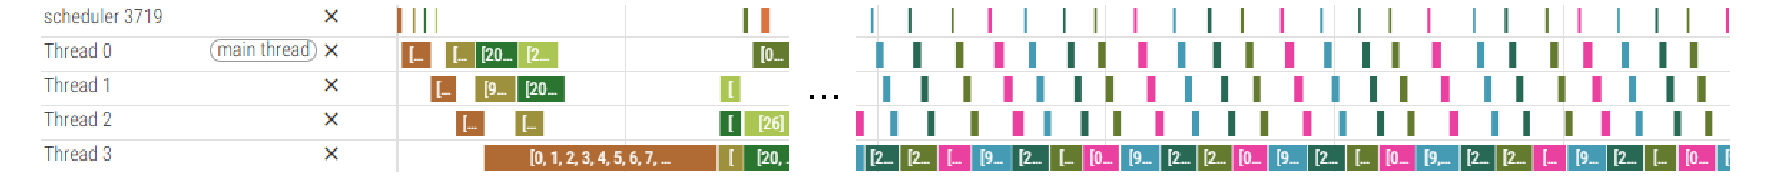
\includegraphics[width=1\linewidth]{figures/trace_lyz_new_new.pdf}
    \caption{An LLM pipeline timeline generated by Perfetto. 
    The data is taken on a system with  4 RTX 3090 GPUs running a four-stage pipeline using the ShareGPT dataset. The different colored blocks represent different batches on each thread running on a GPU, while the white areas indicate pipeline bubbles. It shows that the bubbles begin to emerge and persist after the first few batches due to the limited memory capacity.
    }
    \label{trace}
\end{figure*}

Large Language Models (LLMs) have emerged as a cornerstone of artificial intelligence, demonstrating remarkable applicability to many domains. Significant progress has been reported in code generation\cite{mathews2024test}, text translation\cite{dabre2020survey}, dialogue systems\cite{roller2021recipes} and other applications\cite{lee2024infinigen}. 
To meet increasingly complex application requirements, enhancing the capabilities of LLMs is critical. 
Scaling up the model size has been identified as an effective strategy to achieve this objective\cite{koto-etal-2023-indommlu}. 
Consequently, the size of LLMs has grown exponentially\cite{10549890}, resulting in substantial improvements in their capability and performance. For instance, Llama2-70B exhibits a 42\% improvement in solving mathematical problems compared to its smaller counterpart, Llama2-7B\cite{koto-etal-2023-indommlu}.

As the model size increases, the demand for memory and computational resources also grows, often surpassing the capacity of the host device. 
To address this challenge, employing multi-device clusters for parallel inference and fully leveraging their capabilities have become a key strategy to improve performance.
% rebuttal: 补充是否添加tp
Among various parallel inference techniques, \emph{pipeline parallelism} is a commonly used approach. Technologies such as Google's Gpipe\cite{huang2019gpipe}, Microsoft's DeepSpeed\cite{aminabadi2022deepspeed}, and Nvidia's TensorRT\cite{davoodi2019tensorrt} all leverage pipeline-based parallel inference.
This technology divides the LLM layers into multiple pipeline stages. Each stage is assigned to a separate GPU, thus enables parallel execution across stages. It can significantly enhance the inference throughput and support efficient deployment of LLM.

To fully utilize device resources, the LLM inference engines employ iteration-level schedulers \cite{yu2022orca}, which enhance parallelism by batching tasks at the token-level granularity. 
These advancements mitigate some of the impact caused by the pipeline bubbles and significantly improve the performance, contributing to their widespread adoption \cite{patel2024splitwise, jin2023s, qin2024mooncake}. 
Leading inference frameworks, such as DeepSpeed \cite{aminabadi2022deepspeed}, vLLM \cite{kwon2023efficient}, have integrated such batching techniques.




However, we have observed that this batching cannot fully eliminate the pipeline bubbles. 
We measure GPU utilization using a four-stage pipeline running the workload of the ShareGPT dataset\cite{chiang2023vicuna}. 
The results visualized by Perfetto\cite{perfetto2021} are shown in Figure \ref{trace}.  
There are 4 threads: Threads 0 to 3 with Thread 0 as the Main Thread, each thread on one GPU.
The x-axis shows the elapsed running time.
The figure shows that GPUs are fully utilized only in the first iteration of the inference task, i.e., there is no white space in that period of elapsed time for all threads.
As the inference progresses, pipeline bubbles begin to emerge and persist, shown as white spaces between colored fragments in Threads 0, 1, and 2. Each green fragment represents the execution time for one stage of the inference in a batch running on that thread.
In this scenario, GPUs spend approximately \textbf{60\%} of the time in the stalled state due to the pipeline bubbles. 



A more detailed analysis reveals that this issue is inherent to pipeline-based approaches. 
The primary cause is the mismatch between computational and memory resources in GPUs. 
As illustrated in Figure~\ref{trace}, the formation of bubbles in Threads 0, 1, and 2 is attributed to GPU memory being fully committed.
It prevents the scheduler from assembling new batches until after the completion of the last stage of the previously launched batch. 
It leaves the GPUs for Threads 0,1,2 waiting in an idle state.
Only Thread 3 is fully committed because there is additional computation workload in the last stage of token generation inference, such as projection and token sampling.
This phenomenon highlights a fundamental limitation of the pipeline design, which we will explore further in Section~\ref{sec:pipelinebubble}.

Moreover, although GPUs are idle during the stalled state, they nevertheless continue to draw substantial amounts of power, resulting in unnecessary waste.
Energy efficiency is a critical issue that has garnered significant attention from both academia and industry. 
Existing LLM systems have highlighted such energy efficiency challenges. 
For example, estimates from \cite{patterson2021carbon} indicate that training the GPT-3 model requires 1,287 MWh of energy, equivalent to the annual energy consumption of 420 individuals. 
The energy demands during LLM inference are also noteworthy. Each ChatGPT inference, for instance, consumes approximately 2.9 watt-hours (Wh) of electricity, nearly ten times the 0.3 Wh used by a single Google search\cite{shi2024efficient}.


% Various techniques have been proposed and employed to mitigate the high power and energy usage associated with LLM workloads. 
% For example, NVIDIA GPUs can  adjust power using the \emph{dynamic voltage and frequency scaling (DVFS)} to decrease or increase power ratings based on the workload demands \cite{nvidia}. 
% Existing application-level interfaces on GPUs also support effective software-guided power and energy management. 
% However, due to the overhead of monitoring workload fluctuation and the required latency in power adjustments at runtime, these mechanisms usually operate at the rates of seconds and  with power changes at even longer intervals \cite{chen2023joss}.
% In contrast, each pipeline bubble  typically persists for only a few milliseconds. 
% The coarse resolution prevents most existing schemes from effectively detecting and responding to such brief workload fluctuations, rendering them inadequate for managing power and energy changes in this context.

% Various techniques have been proposed and employed to mitigate the high energy comsumpation while not affecting the performance. 
% 硬件层面，英伟达GPU能够自动检测任务负载的变化，从而动态调节GPU的电压和频率(DVFS)
% 用户层面，人工可以通过NVML指令动态调节GPU的频率，降低位于非critical-path上的computation的频率，实现节能的效果。
% 然而，GPU频率调节的时间粒度是几个到几十个milliseconds，which 和气泡的时间相等 during inference。
% 这使得it hard to 动态调节频率来消除bubble处的能耗
% \bylyz{
Various techniques have been proposed to optimize energy efficiency in LLM workloads without compromising performance.
NVIDIA GPUs can autonomously detect workload fluctuations and dynamically modulate power via dynamic voltage and frequency scaling (DVFS)~\cite{nvidia}. 
ThrottLL'eM~\cite{kakolyris2025throttll} analyzes the impact of GPU frequency on LLM  energy efficiency, employing dynamic frequency scaling informed by environmental factors to enhance efficiency. 
Perseus~\cite{chung2024reducing} dynamically lowers frequencies for non-critical-path computations to mitigate energy consumption through manual frequency adjustments. 
Nonetheless, the overhead of these GPU adjustment mechanisms ranges from several to tens of milliseconds~\cite{chen2023joss}, a timescale commensurate with the duration of pipeline bubbles during inference. 
This equivalence renders dynamic GPU regulation ineffective for decreasing energy waste within these bubbles.
% }



To address these issues, we propose a counterintuitive strategy.
% Instead of using DVFS to lower power when bubbles occur, we reduce the GPU’s \textit{frequency} (the configurable upper bound on its power consumption) to slow computation, thereby preventing bubble formation. 
\bylyz{
Instead of dynamically setting the frequency when bubble occur, we staticly reduce the GPU's frequency to slow computation, thereby preventing bubble formation. 
As discussed earlier, bubbles in Threads 0, 1, and 2 arise from a mismatch between GPU compute and memory resources. 
In our proposed approach, instead of using full frequency to process the required stage of a batch and then wait for memory resources to become available for the next batch (i.e., to form a bubble), we intentionally lower the frequency to slow down the computation of each batch, which can then match the time when memory resource is released and becomes available.
}


Ideally, if the completion time of the first stage in the current batch is delayed sufficiently to align with the finish time of a previously launched batch in the last stage, no pipeline bubbles will form. 
As a batch finished, the scheduler can initiate the construction of a new batch in time.
The alignment ensures that the subsequent inference batch is ready just as Thread 0 completes its current batch, i.e. eliminating the bubbles on Thread 0.
Additionally, the extended execution time of stages across multiple batches enables them to be more closely connected, reducing bubbles between stages, as the colored fragments in Figure \ref{trace} will be extended to replace the white space following them.
Such frequency adjustments are much more manageable because they are at a coarser grain (i.e., applied to all colored fragments) than that of individual bubbles (more details in Section~\ref{sec:pipelinebubble}).


To reduce these bubbles during inference presents several challenges.
\bylyz{
First, the optimal GPU frequency must be determined within a minimal profiling time to maintain low overhead. 
Second, the targeted frequency configuration must be highly precise to maximize bubble reduction without compromising inference performance.
Third, the framework should possess broad generalizability across diverse hardware platforms and various pipeline-parallel LLM architectures.
}

% \bygpt{
% Reducing pipeline bubbles during inference through static GPU frequency adjustment presents three challenges.
% First, suitable frequencies must be identified with low tuning overhead.
% Second, the selected frequencies must be based on accurate estimates of stage execution time, allowing faster stages to exploit available pipeline slack while limiting performance degradation.
% Third, the framework should be applicable across different hardware platforms and LLMs deployed with pipeline parallelism.
% }
% First, high-resolution power scaling is not available. 
% Current GPU power management cannot operate at the level of milliseconds required to respond to individual pipeline bubbles effectively. 
% This limitation is primarily due to the inherent latency of power-scaling operations and the constraints of existing hardware and firmware designs\cite{chen2023joss}.
% Second, accurately controlling the execution time of LLM inference to prevent the formation of bubbles by power scaling is non-trivial. 
% Third, the proposed framework should be general and applicable to different machine platforms and different pipeline-based LLM models.


% To tackle these challenges, we quantify the relationship between iteration-level batch latency and the GPU’s power rating for a given model. 
% Although input data might seem to influence iteration latency, we find it is largely determined by the model’s configuration and power setting, \bygxl{due to the heavy computation over fixed model parameters}(more details are discussed in Section~\ref{sec:stableexecutiontime}). 
% \bygxl{!!!REWrite this paragraph!!!Although input data might seem to influence iteration latency, we find it is largely determined by the model’s configuration and power setting, due to the advancements in long-context processing optimizations and heavy computation over fixed model parameters (more details are discussed in Section~\ref{sec:stableexecutiontime}).} 
% However, the batch lantency is also influenced by the 这个batch中的sequence length和batchsize，which is hard to predict and control during the iteration.
% However, we found the impact is negligible during the decode phase, where we focused, due to the advancements in long-context processing optimizations and heavy computation over fixed model parameters (more details are discussed in Section~\ref{sec:stableexecutiontime}).
% \bylyz{Although batch latency is also theoretically influenced by sequence length and batch size which are hard to predict and controlled during the runtime, we find their impact to be negligible during decoding phase where we focus, due to  advances in long-context optimization and the dominant cost of computations over fixed model parameters (more details are discussed in Section~\ref{sec:stableexecutiontime}).}
% Leveraging this input-insensitive property, we build an analytical model through one-time profiling of a small set of batched iterations in a pipeline-parallel LLM. 
% This model enables the host GPU to set power ratings that align stage completion times and eliminate pipeline bubbles.

To address these challenges, we conduct a thorough study on the behavior of the LLM inference tasks.
Firstly, we find that the iteration-level batch execution time of a given model during LLM inference is stable and largely input-insensitive, as it is dominated by the model’s heavy parameter loading and high parallel computation capacity(see Section~\ref{sec:stableexecutiontime}). 
Based on this observation,  an analytical model can be established by one-time profiling of a limited number of batched iterations in a pipeline-based LLM model.
This model provides actionable guidance to set the frequency of GPUs and effectively reduce pipeline bubbles. 



In this paper, we propose \thisproj{}, a general framework that regulates GPU frequency to optimize energy efficiency in pipeline-based LLM inference engines.
We develop an analytical model capturing the relationship between GPU frequency and execution time of stages in the LLM pipelines. 
Guided by this model, \thisproj{} reduces pipeline bubbles, enabling significant power efficiency improvements with minimal performance impact.
We have proved the effectiveness of \thisproj{} on both \hcwplaceholder{XXX} and \hcwplaceholder{XXX} and our experiments show up to \hcwplaceholder{XX}\% energy efficiency improvement, with average improvements of \hcwplaceholder{XXX}\% on Llama3-8B and \hcwplaceholder{XXX}\% on Llama3-70B.
In summary, we make the following contributions.

\begin{itemize}
\item 
We analyze iteration-level batch inference in pipeline-parallel LLMs, showing that inevitable bubbles arise from stage execution time misalignment caused by compute–memory mismatches. 
We further demonstrate that stage execution times are largely input-insensitive, offering opportunities for optimization.

\item We propose \thisproj{}, an LLM inference optimization framework that reduces pipeline bubbles through model-guided static frequency adjustments.
It constructs a quantitative analytical model, leveraging input-insensitive execution time characteristics, to describe the relationship between energy efficiency and performance based on offline, one-time profiling.
The approach is general and effective across diverse LLM inference engines.

\item We have implemented \thisproj{} for state-of-the-art pipeline-based LLM inference engines using continuous batching \cite{yu2022orca}. 
Extensive experiments demonstrate that \thisproj{} improve energy efficiency by up to \hcwplaceholder{XXX}\%, with an average reduction of \hcwplaceholder{XXX}\% on Llama3-8B and \hcwplaceholder{XXX}\% on Llama3-70B, al  l while maintaining the inference engine's high performance.
\end{itemize}


The rest of the paper is organized as follows. Section~\ref{sec:background} provides necessary background about LLM inference.
Section~\ref{sec:design} presents the design and implementation of \thisproj{}. 
Section~\ref{sec:evaluation} evaluates \thisproj{} with various benchmarks and discussed the experimental results. 
% Then, Section~\ref{sec:relatedworks} discussed some other works related to our work. 
% Section~\ref{sec:discussion} discusses our work's applicability and limitations
Section \ref{sec:relatedworks} reviews related work.
Section \ref{sec:discussion} discusses the applicability and limitations of our approach.
Finally, section \ref{sec:conclusion} concludes the paper.







\section{Background and Motivation}
\label{sec:background}

\subsection{LLM Architecture and Parallel Stategy}
\label{sec:llmandtransformer}

% \begin{figure}
% 	\centering
% 	\begin{minipage}[t]{\linewidth}
% 		\centering
% 		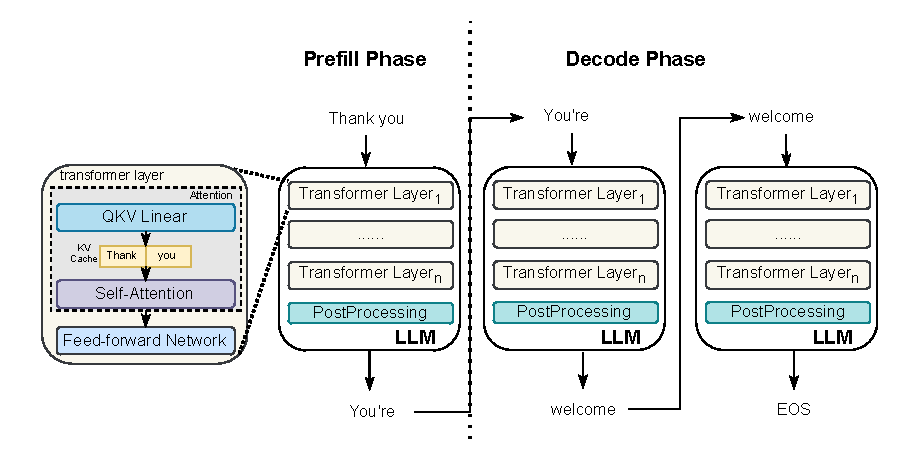
\includegraphics[width=3.3in]{figures/inference_phase_new_new_new.pdf}
% 		\caption{The inference process of a transformer-based LLM model}
% 		\label{fig:inferencephase}
% 	\end{minipage}
% 	\begin{minipage}[t]{\linewidth}
% 		\centering
% 		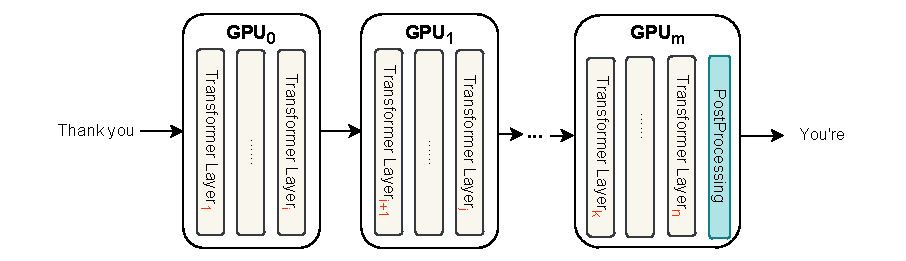
\includegraphics[width=3.3in]{figures/parallel_new_new_new.pdf}
% 		\caption{The pipelined parallelism}
% 		\label{Pipeline Parallelism}
% 	\end{minipage}
%     \label{LLM architecture}
% \end{figure}

% \begin{figure}[t] % 使用 [t] 尽量让图片置顶，符合论文习惯
%     \centering
%     % 第一张子图
%     \begin{subfigure}{\linewidth}
%         \centering
%         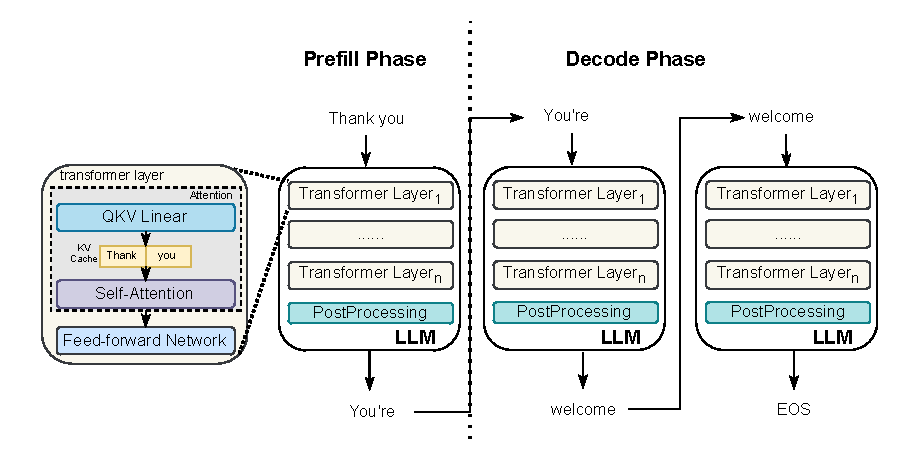
\includegraphics[width=3in]{figures/inference_phase_new_new_new.pdf}
%         \caption{The inference process of a transformer-based LLM model}
%         \label{fig:inferencephase}
%     \end{subfigure}
    
%     \vspace{1em} % 调节两张图之间的垂直间距，可以根据需要缩小或放大
    
%     % 第二张子图
%     \begin{subfigure}{\linewidth}
%         \centering
%         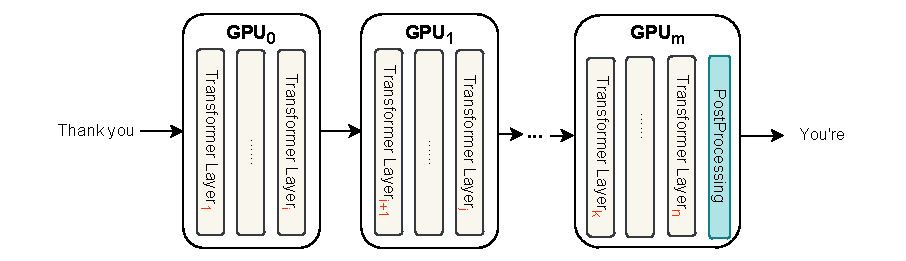
\includegraphics[width=3in]{figures/parallel_new_new_new.pdf}
%         \caption{The pipeline parallelism}
%         \label{Pipeline Parallelism}
%     \end{subfigure}
    
%     \caption{Overview of LLM inference and pipeline parallelism.} % 总标题
%     \label{fig:llm_architecture}
% \end{figure}

% \begin{figure}[t]
%     \centering
%     \begin{minipage}[t]{0.48\textwidth}
%         \centering
%         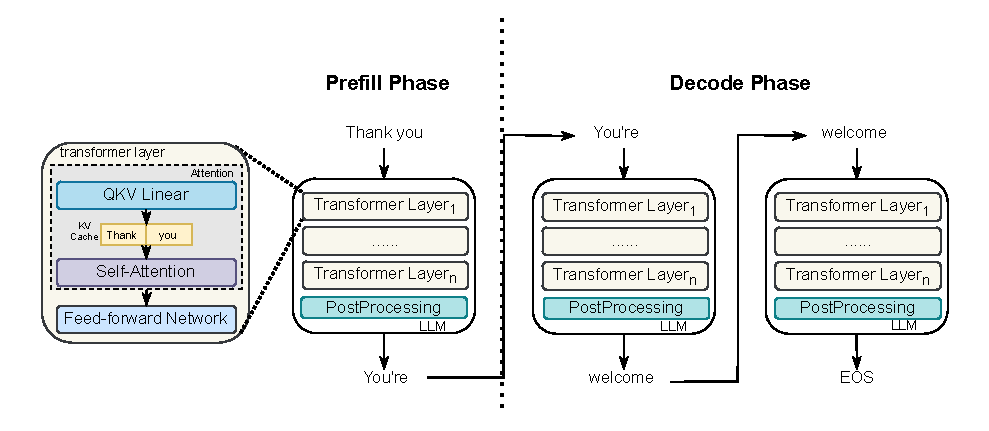
\includegraphics[width=\textwidth]{figures/inference_phase_new_new.pdf}
%         \caption{The inference process of a transformer-based LLM model}
%         \label{fig:inferencephase}
%     \end{minipage}
%     \hspace{0.02\textwidth}
%     \begin{minipage}[t]{0.48\textwidth}
%         \centering
%         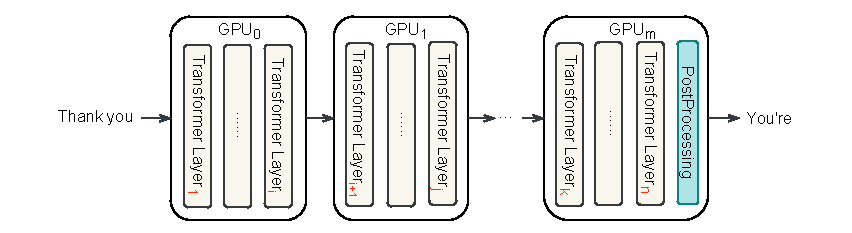
\includegraphics[width=\textwidth]{figures/parallel_new_new.pdf}
%         \caption{The pipelined parallelism}
%         \label{Pipeline Parallelism}
%     \end{minipage}
% \end{figure}

% \begin{figure}[t]
%     \centering
%     \begin{minipage}[t]{0.48\textwidth}
%         \centering
%         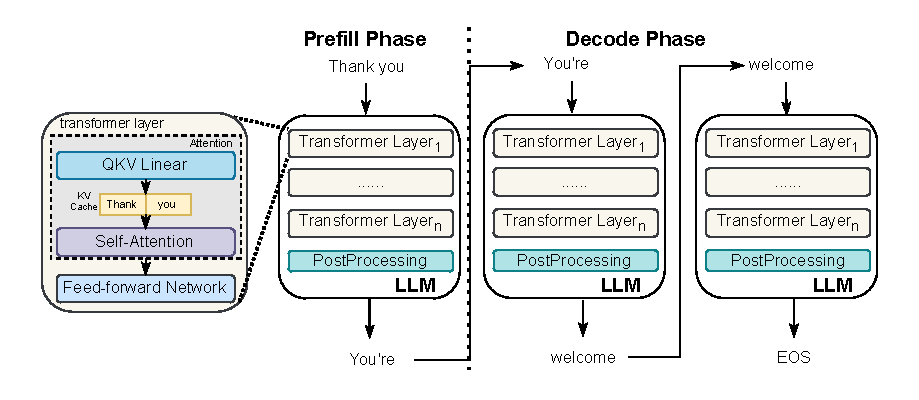
\includegraphics[width=\textwidth]{figures/inference_phase_new_new_new_new.pdf}
%         \caption{The inference process of a transformer-based LLM model}
%         \label{fig:inferencephase}
%     \end{minipage}
%     \hspace{0.02\textwidth}
%     \begin{minipage}[t]{0.48\textwidth}
%         \centering
%         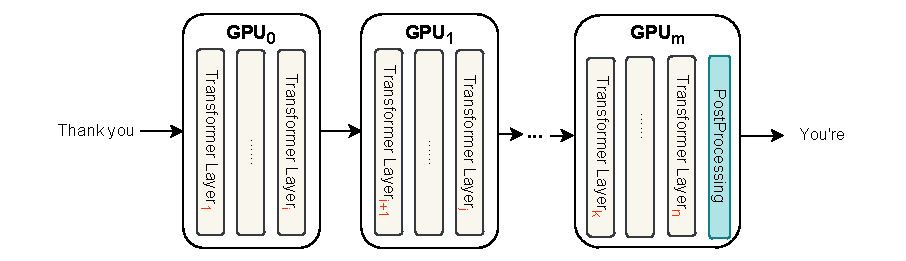
\includegraphics[width=\textwidth]{figures/parallel_new_new_new.pdf}
%         \caption{The pipelined parallelism}
%         \label{Pipeline Parallelism}
%     \end{minipage}
% \end{figure}

% \begin{figure}[t]
%     \centering
%     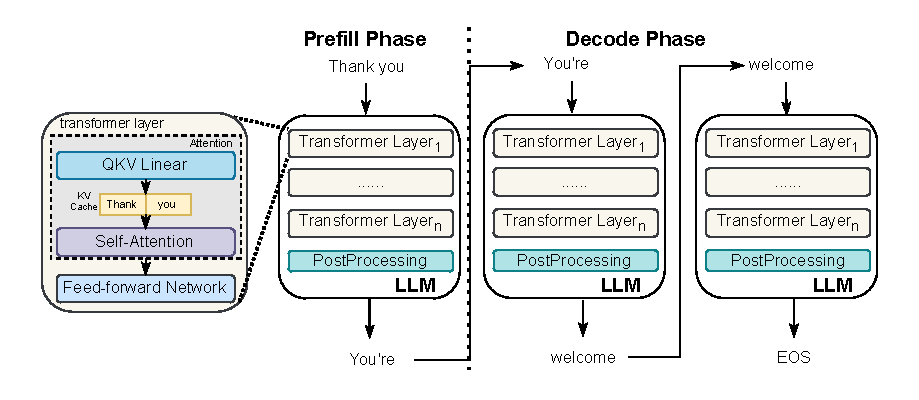
\includegraphics[width=0.48\textwidth, valign=m]{figures/inference_phase_new_new_new_new.pdf}
%     \hfill
%     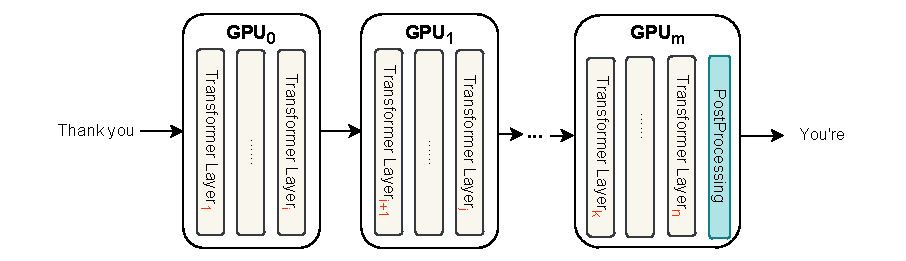
\includegraphics[width=0.48\textwidth, valign=m]{figures/parallel_new_new_new.pdf}
%     \begin{minipage}[t]{0.48\textwidth}
%         \caption{The inference process of a transformer-based LLM model.}
%         \label{fig:inferencephase}
%     \end{minipage}
%     \hfill
%     \begin{minipage}[t]{0.48\textwidth}
%         \caption{The pipelined parallelism mechanism.}
%         \label{Pipeline Parallelism}
%     \end{minipage}
% \end{figure}

% \begin{figure}[t]
%     \centering
%     % --- 第一行：图片部分（垂直居中对齐） ---
%     \begin{minipage}[c]{0.48\textwidth}
%         \centering
%         % 使用 \vfill 确保图片在 minipage 内部居中，或配合 \raisebox
%         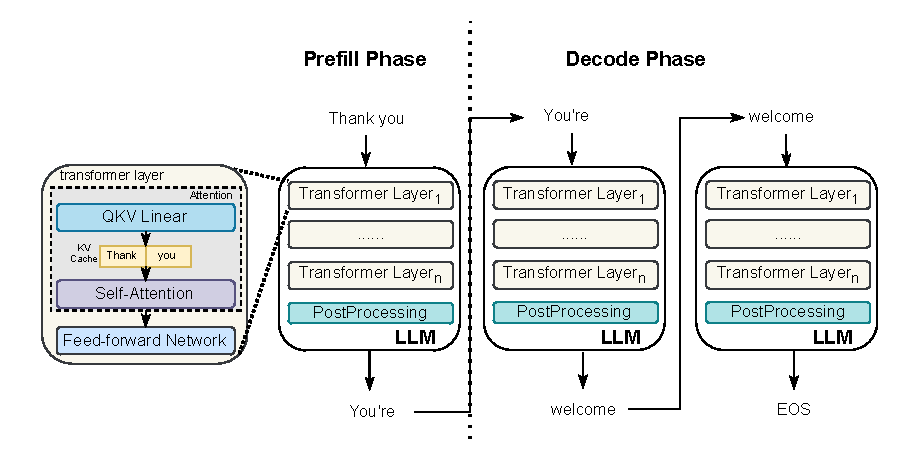
\includegraphics[width=\textwidth]{figures/inference_phase_new_new_new.pdf}
%     \end{minipage}
%     \hfill
%     \begin{minipage}[c]{0.48\textwidth}
%         \centering
%         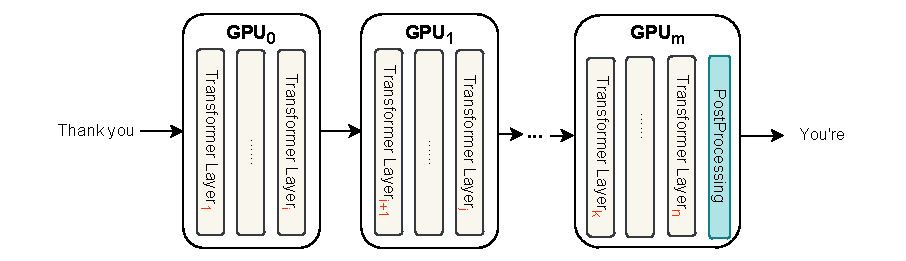
\includegraphics[width=\textwidth]{figures/parallel_new_new_new.pdf}
%     \end{minipage}

%     \vspace{5pt} % 调节图片与标题之间的间距

%     % --- 第二行：标题部分（顶端对齐，确保 Caption 对齐） ---
%     \begin{minipage}[t]{0.48\textwidth}
%         \caption{The inference process of a transformer-based LLM model}
%         \label{fig:inferencephase}
%     \end{minipage}
%     \hfill
%     \begin{minipage}[t]{0.48\textwidth}
%         \caption{The pipelined parallelism}
%         \label{Pipeline Parallelism}
%     \end{minipage}
% \end{figure}

% \begin{figure}[t]
%     \centering
%     % 创建一个两列表格，列宽各占约一半
%     \begin{tabular}{m{0.48\textwidth} m{0.48\textwidth}}
%         % --- 第一行：放图片 ---
%         \centering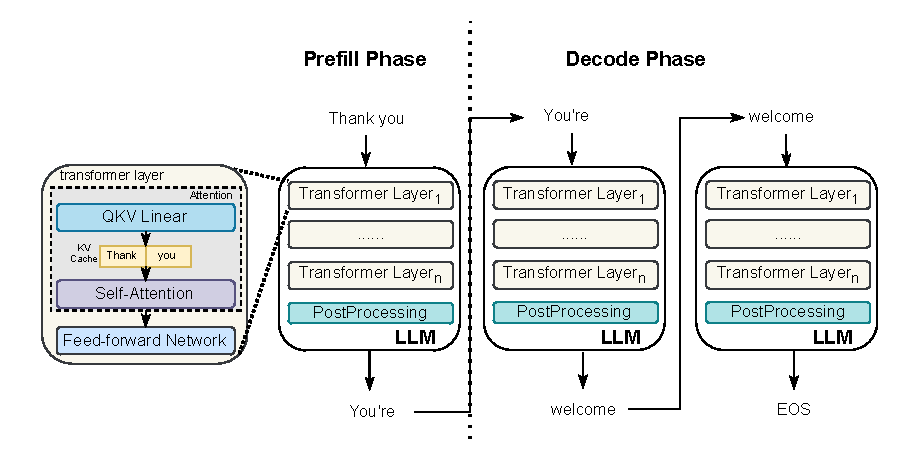
\includegraphics[width=0.45\textwidth]{figures/inference_phase_new_new_new.pdf} & 
%         \centering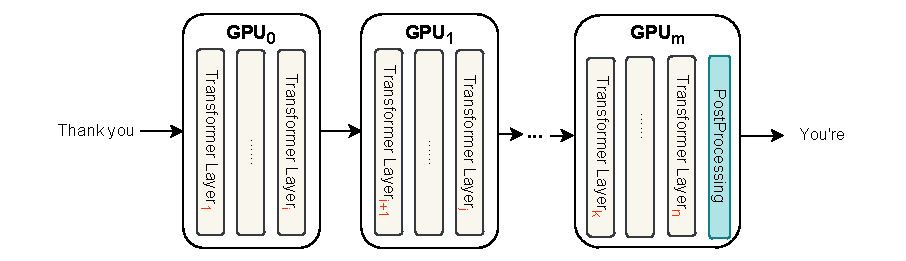
\includegraphics[width=0.45\textwidth]{figures/parallel_new_new_new.pdf} \\
        
%         % --- 第二行：放标题 ---
%         \begin{minipage}[t]{0.48\textwidth}
%             \caption{The inference process of a transformer-based LLM model}
%             \label{fig:inferencephase}
%         \end{minipage} & 
%         \begin{minipage}[t]{0.48\textwidth}
%             \caption{The pipelined parallelism}
%             \label{Pipeline Parallelism}
%         \end{minipage}
%     \end{tabular}
% \end{figure}

% \begin{figure}[t]
%     \centering
%     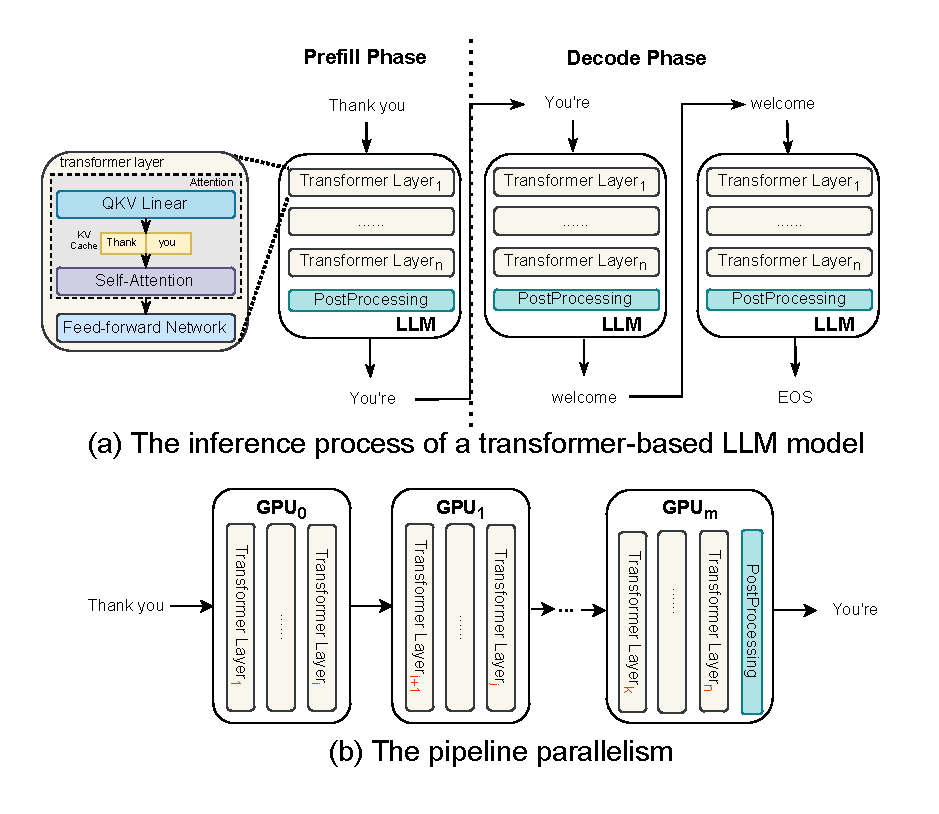
\includegraphics[width=0.7\linewidth]{figures/inference_phase_parallel.pdf}
%     \caption{Overview of LLM inference and pipeline parallelism.}
%     \label{fig:llm_architecture}
% \end{figure}

% Mainstream LLMs, such as ChatGPT \cite{achiam2023gpt}, Llama \cite{touvron2023llama}, and Gemini \cite{team2023gemini}, are built upon the transformer architecture, which consists of a sequence of identical transformer layers (referred to as "layers"). 
% Each layer contains two primary components: the \textit{Attention} and the \textit{Feed-Forward Network (FFN)}. 
% In the Attention, the input embeddings are projected into Query (Q), Key (K), and Value (V) vectors, and the interaction between Q and KV produces the attention outputs. 
% The FFN then further transforms these attention outputs through weight matrices to generate a hidden state as the input vector for the next layer. 
% As illustrated in Figure~\ref{fig:inferencephase}, an LLM processes $n$ layers sequentially within each iteration, producing a single token only after all layers are traversed. 
% This procedure repeats until an end-of-sequence (EOS) token is generated, with each iteration’s output concatenated with the prior context as input to the next iteration.

\bylyz{
An LLM consists of a sequence of Transformer layers (referred to simply as layers).
Each layer comprises an Attention module and a Feed-Forward Network (FFN). 
Within the Attention module, the input representation is first projected into Query ($Q$), Key ($K$), and Value ($V$) matrices. 
$Q$ then attends to $K$ and $V$ via scaled dot-product and Softmax operations to produce the output. 
The FFN subsequently takes the Attention output as input and performs two dense matrix multiplications to generate the input for the next layer. 
Finally, the hidden state output by the final layer undergoes an additional matrix multiplication and Softmax operation to sample from the vocabulary and generate the next token—a phase we denote as postprocessing.
}

% \bygpt{
% A decoder-only transformer LLM consists of a stack of transformer layers (hereafter referred to as layers). Each layer contains two main components: an attention module and a feed-forward network (FFN). The attention module first projects input hidden states into query (Q), key (K), and value (V) representations. Scaled dot products between Q and K are causally masked and normalized with softmax to obtain attention weights, which are applied to V to produce the attention output. The FFN then transforms the resulting hidden states through linear projections and nonlinear activations. Standard FFNs use two linear projections, whereas gated FFNs, such as those in Llama, use three. After the final layer, an output projection maps the hidden state to vocabulary logits. For sampling, softmax converts these logits into a probability distribution from which the next token is drawn. We refer to output projection and token selection together as postprocessing.
% }

% \bygemini{
% An LLM consists of a sequence of Transformer layers (referred to simply as layers). Each layer comprises an Attention module and a Feed-Forward Network (FFN). Within the Attention module, the input representation is first projected into Query ($Q$), Key ($K$), and Value ($V$) matrices. $Q$ then attends to $K$ and $V$ via scaled dot-product and Softmax operations to produce the output. The FFN subsequently takes the Attention output as input and performs two dense matrix multiplications to generate the input for the next layer. Finally, the hidden state output by the final layer undergoes an additional matrix multiplication and Softmax operation to sample from the vocabulary and generate the next token—a phase we denote as postprocessing.
% }

% Due to their distinct computational characteristics, the inference process can be divided into two phases:  
% \textbf{Prefill Phase:} The model processes the entire user request to generate the first token.  
% \textbf{Decode Phase:} The model then generates subsequent tokens in an auto-regressive manner, where each new token depends on all previously generated tokens.  
% Most LLM inference optimizations focus on the decode phase, as it accounts for the majority of inference time.

% During decoding, each newly generated Query must attend to all preceding Keys and Values to compute the attention output.
% We denote the number of preceding tokens as the \textit{sequence length}.
% Accordingly, the computational cost of the attention layer scales linearly with the \textit{sequence length}.
% To eliminate redundant recomputation of earlier KV pairs, LLMs employ a \textbf{KV-Cache}, which stores previously computed Keys and Values for direct reuse in subsequent iterations.
% In contrast, the FFN layer performs fixed-size matrix multiplications between the attention output and model parameters, making its computational cost independent of the sequence length.

% To improve computational efficiency and resource utilization, modern LLM inference engines adopt \textit{batching}, wherein multiple user requests are processed together as a single batch.
% Because LLMs contain an extremely large number of parameters, the cost of parameter loading is non-negligible.
% By aggregating embeddings from different requests into a matrix, batching allows computations to be executed as matrix multiplications instead of repeated vector operations and parameter loading, thereby enhancing efficiency.
% The number of requests processed together defines the \textit{batch size}.
% Consequently, the computational workload of a transformer layer increases proportionally with the batch size, in addition to a fixed but dominant parameter loading overhead.

\bylyz{
LLMs primarily operate in two phases: prefill and decode. 
During the prefill phase, the model processes the entire user request to generate the first output token. 
In the decode phase, it generates subsequent tokens iteratively using the newly generated token along with all preceding tokens, the count of which is referred to as the sequence length. 
This decoding loop repeats until an end-of-sequence (EOS) token is produced.
To avoid redundant Query-Key-Value (QKV) recalculations for previous tokens, LLMs employ a KV-Cache to store previously computed key and value states, loading them dynamically when needed.
Furthermore, to enhance computational efficiency, LLMs adopt batching, combining multiple user requests into a single batch to amortize the heavy overhead of loading model parameters. 
The total number of aggregated requests in a batch is defined as the batch size.
}

% \bygpt{
% LLM inference consists of two phases: prefill and decode. During prefill, the model processes the entire input prompt to produce the first output token. During decode, it generates subsequent tokens autoregressively, using the most recently generated token together with the preceding context. We use sequence length to denote the number of preceding context tokens, including prompt tokens and earlier generated tokens. Decoding continues until an end-of-sequence (EOS) token is generated or another stopping condition is met. To avoid recomputing the keys and values of previous tokens, the model stores them in a KV cache for reuse in subsequent iterations.
% To improve computational efficiency, inference engines group multiple requests into a batch, amortizing the cost of loading model parameters across these requests. The number of requests processed together in a batch is referred to as the batch size.
% }

% \bygemini{
% LLMs primarily operate in two phases: prefill and decode. During the prefill phase, the model processes the entire user request to generate the first output token. In the decode phase, it generates subsequent tokens iteratively using the newly generated token along with all preceding tokens, the count of which is referred to as the sequence length. This decoding loop repeats until an end-of-sequence (EOS) token is produced. To avoid redundant Query-Key-Value (QKV) recalculations for previous tokens, LLMs employ a KV-Cache to store previously computed key and value states, loading them dynamically when needed. Furthermore, to enhance computational efficiency, LLMs adopt batching, combining multiple user requests into a single batch to amortize the heavy overhead of loading model parameters. The total number of aggregated requests in a batch is defined as the batch size.
% }

\bylyz{
When an LLM becomes too large to fit on a single GPU, model parallelism distributes its parameters and computation across multiple GPUs.
Common strategies include tensor parallelism (TP), pipeline parallelism (PP), and expert parallelism (EP). 
TP partitions weight matrices within layers across GPUs and uses collective communication to combine intermediate results.
PP assigns groups of consecutive layers to different GPUs, which exchange activations at stage boundaries. 
Compared with TP, PP typically requires less frequent communication and can be more suitable for deployments with limited interconnect bandwidth, such as systems using PCIe.
EP targets mixture-of-experts (MoE) models, in which MoE layers contain multiple expert FFNs. 
It distributes these experts across GPUs and routes tokens to the selected experts.
Our work focuses on PP, while extensions involving other parallelism strategies are discussed in Section~\ref{sec:discussion}.
}

% \bygpt{
% When an LLM becomes too large to fit on a single GPU, model parallelism distributes its parameters and computation across multiple GPUs. Common strategies include tensor parallelism (TP), pipeline parallelism (PP), and expert parallelism (EP). TP partitions weight matrices within layers across GPUs and uses collective communication to combine intermediate results. PP assigns groups of consecutive layers to different GPUs, which exchange activations at stage boundaries. Compared with TP, PP typically requires less frequent communication and can be more suitable for deployments with limited interconnect bandwidth, such as systems using PCIe. EP targets mixture-of-experts (MoE) models, in which MoE layers contain multiple expert FFNs. It distributes these experts across GPUs and routes tokens to the selected experts. Our work focuses on PP, while extensions involving other parallelism strategies are discussed in Section~\ref{sec:discussion}.
% }

% \bygemini{
% As models grow larger and exceed the memory capacity of a single GPU, various parallel strategies have been proposed to shard parameters across multiple GPUs. The most commonly used strategies include Tensor Parallelism (TP), Pipeline Parallelism (PP), and Expert Parallelism (EP). Tensor Parallelism shards the weight matrices across GPUs, whereas Pipeline Parallelism partitions the model layer-by-layer. Pipeline Parallelism typically incurs lower communication overhead than Tensor Parallelism, making it better suited for systems with limited inter-GPU bandwidth, such as PCIe-interconnected nodes. Meanwhile, Expert Parallelism targets Mixture-of-Experts (MoE) models, where standard Feed-Forward Networks (FFNs) are replaced by multiple expert FFNs distributed across GPUs. Our work primarily focuses on the Pipeline Parallelism scenario, while other parallel strategies are discussed in Section \ref{sec:discussion}.
% }

%attention 和FFN都在干什么，矩阵乘法？里面有大量的参数需要加载，然后和输入的数据运算
%同时，还要和已经生成的数据运算
%因此一个layer的时间包括了模型加载，包括了blablabla，分别和什么相关。
%这样后面也可以说，batch其实是在提升这些数据的利用效率

% To improve computational efficiency and resource utilization, modern LLM inference engines adopt \textbf{batching}, where multiple user requests are processed simultaneously. 
% Specifically, embeddings from different requests are aggregated into a single matrix, allowing the computation to be executed as matrix multiplications rather than individual vector operations. 
% This design also enables model parameters, including those used for QKV projection and the FFN transformation, to be loaded once and reused across all requests in the batch, thereby reducing redundant memory accesses.
% The benefit of batching is particularly pronounced during the decode phase, where inference is typically dominated by parameter loading rather than arithmetic operations.
% \bygxl{!!!start the batch execution story here!!!}
%这里应该简单的提一句，batch的大小其实影响的是输入矩阵的大小，因此batch-size是每一个layer的推理时间的重要影响因素，就可以了。

% To improve computational efficiency and resource utilization, modern LLM inference engines adopt \textit{batching}, wherein multiple user requests are processed together as a single batch.
% Because LLMs contain an extremely large number of parameters, the cost of parameter loading is non-negligible.
% By aggregating embeddings from different requests into a matrix, batching allows computations to be executed as matrix multiplications instead of repeated vector operations and parameter loading, thereby enhancing efficiency.
% The number of requests processed together defines the \textit{batch size}.
% Consequently, the computational workload of a transformer layer increases proportionally with the batch size, in addition to a fixed but dominant parameter loading overhead.

% To enhance computational efficiency and resource utilization, LLMs typically batch multiple users' requests for inference by combining their embeddings into a matrix. 
% Matrix multiplications thus serve as the core operations and accounts for the majority of the inference time \cite{zhong2024distserve}. 
% The end-to-end execution time is also determined by the sizes of the input matrix and the parameter matrix, which in turn are dictated by the model size and the batch size.
% It is insensitive to the values stored in the matrices. 
% \bylyz{There}


% Due to differences in computational characteristics, the inference process is divided into two distinct phases:
% \textbf{Prefill Phase:} In this phase, the model processes the user’s request to generate the first token.
% \textbf{Decode Phase:} During this phase, the model generates subsequent tokens one-by-one in an auto-regressive manner. 
% The iterative nature of the model during decoding means that each new token is computed based on all previously generated tokens in the sequence. Specifically, the model relies on the Query, Key, and Value (QKV) matrices of the preceding tokens, leading to redundant regeneration of the Key and Value matrices for earlier tokens. 
% To mitigate this redundancy, LLMs store the previously computed Key and Value pairs in a \textbf{KV-Cache}. 
% As a result, the workload for generating each token is linearly proportional to the length of the sequence already generated. 
% This involves loading the KV pairs from the KV-Cache and computing the attention scores based on these stored values.





% % \notethis{say some conclusions about LLM inference}
%这里要说，有大量的计算，有大量的参数，因此GPU成了首选的计算设备
%还要说这个东西填不满一个GPU的算力，因此要做batch，我记得上一个论文里写了一段类似的话
%一个batch里面，session的多少，受到了GPU显存的限制
%别忘了在这一节的前半部分要强调这些tf block是相互独立的，结构都差不多，这样为后面引入流水线做文字上的铺垫

\subsection{Inevitable Bubbles in Pipeline-Based LLM Inference}
\label{sec:pipelinebubble}
%承担上文
%大模型的尺寸变大了，一个显卡放不下，需要多块卡共同存储，因此多卡也搞并行
%然后可以直接跳到，因为各个tf block是独立的，按块切开做流水是一个很直观的思路。注意就不要提其他的并行了，容易把主题搞散了

% LLM models impose intense memory pressure due to the large number of parameters in the transformer layers. 
% For instance, Llama2-70B consists of 80 layers, with each layer containing approximately 1 billion parameters.
% Additionally, the KV-Cache increases as the inference process progresses, consuming a substantial portion of GPU memory \cite{jin2023s}. 
% As a result, GPU memory capacity becomes a limiting factor for the number of layers and batches that can be deployed.

% Therefore, models are sharded across multiple GPUs in modern inference engines.
% This allows for larger batches, higher throughput, and more efficient inference.
% Pipeline parallelism (Figure~\ref{Pipeline Parallelism}) is a common strategy \cite{huang2019gpipe, rasley2020deepspeed}, where the \texttt{n} transformer layers are split into \texttt{m} stages, each on a separate GPU.
% Batches flow sequentially through the stages, and each GPU starts processing the next batch immediately after finishing the current one, boosting throughput.
% In the last stage, generated tokens are fed back to the first stage for the next iteration until an \texttt{EOS} token ends the process.

% Reducing pipeline bubbles is key to optimizing LLM inference.
\bylyz{Bubbles are commonly existed in the Pipeline Parallel and reducing these bubbles is key to optimizing LLM inference.}
Proposed solutions include stage alignment \cite{lin2024syncintellects,zheng2024response,jin2023s}, virtual pipeline stages \cite{narayanan2021efficient,jiang2024dynapipe}, and continuous batching \cite{yu2022orca}, the most widely used approach. 
In continuous batching, queued requests are grouped before inference, and new requests are added after each iteration when completed requests free enough GPU memory. 
This improves scheduling flexibility and GPU utilization \cite{achiam2023gpt,rasley2020deepspeed,devlin2018bert}.



\begin{figure}[t]
    \centering
    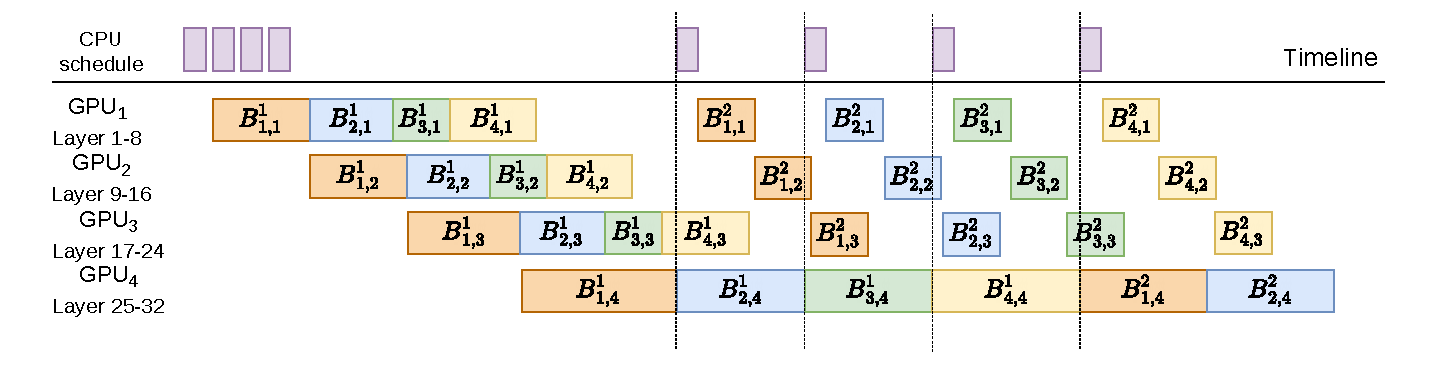
\includegraphics[width=0.9\linewidth]{figures/TACO_Rebuttal/workflow1_new.pdf}
    \caption{A schematic diagram of the timeline for a four-stage pipeline using continuous batching.}
    \label{workflow}
\end{figure}

Our observation shows that continuous batching cannot fully remove pipeline bubbles due to limited GPU memory.
Figure~\ref{workflow} illustrates a four-stage pipelined workflow utilizing continuous batching.
In this configuration, a 32-layer LLM is partitioned across four GPUs, with each GPU assigned a consecutive block of eight layers, forming one pipeline stage.
The purple segments indicate work performed by the CPU scheduling thread, which assembles batches by collecting requests from the waiting queue.
When a request reaches an \texttt{EOS} token, the scheduler returns the result to the user and releases its associated GPU memory.
Simultaneously, it schedules new requests to form the next batch.
Otherwise, it remains in the batch and proceeds to the next token generation iteration.
The brown, blue, green, and yellow segments represent inference threads on the GPUs, each responsible for executing a specific computational batch.
Specifically, $B_{i,j}^k$ denotes the $i$-th batch running on the $j$-th GPU (i.e., the $j$-th stage of the pipeline) during the $k$-th iteration, corresponding to generation of the $k$-th token.


\iffalse
\begin{table}
  \caption{Computational cost of various operations involved in generating a single token during the decoding phase, assuming a sequence length of 4096. "TL" denotes Transformer Layers, "P" denotes Projection and "S" denotes Sampling. $n$ denotes the number of transformer layers, and $N$ denotes the number of pipeline stages.}
  \label{tab:computation}
  \begin{tabular}{ccccc}
    \toprule
    \multirow{2}{*}{Model} & \multicolumn{3}{c}{Computation (GFLOPs)} & \multirow{2}{*}{Performance} \\
    \cmidrule{2-4}
     & TL & P+S & TL Per Stage \\
    % \midrule
    % Llama2-7B & \multirow{2}{*}{8.99 GFLOPs} & \multirow{2}{*}{0.26 GFLOPs} \\
    % $(n=32)$ & & \\
    \midrule
    Llama3-8B & \multirow{2}{*}{9.93} & \multirow{2}{*}{1.05} & \multirow{2}{*}{2.48 $(N=4)$} & \multirow{2}{*}{\Checkmark} \\
    $(n=32)$ & & & & \\
    \midrule
    Llama3-70B & \multirow{2}{*}{59.73} & \multirow{2}{*}{2.10} & 14.93 $(N=4)$ & \XSolidBrush \\
    $(n=80)$ & & & 7.47 $(N=8)$ & \Checkmark \\
    \bottomrule
  \end{tabular}
\end{table}
\fi

% memory constraint 导致了schedule的delay
At the start of an inference, the CPU scheduling thread and the inference thread on GPU$_1$ can run in parallel. 
While GPU$_1$ begins processing one batch, the CPU scheduler simultaneously constructs subsequent batches from the waiting queue to enable continuous batching inference. 
However, as the inference process advances, the available GPU memory capacity will be exhausted leaving insufficient memory to accommodate new batches.
In this case, the CPU must wait for the ongoing batch to complete before scheduling the next batch.
During this period, GPU$_1$ will be forced to stall and create a pipeline bubble.
This delay (or bubble) can ripple through the rest of the pipeline.  
As shown in Figure~\ref{workflow}, before the batch $B_{1,1}^2$ begins its execution, the CPU scheduling thread must wait for batch $B_{1,4}^1$ to complete its last stage on $\text{GPU}_{4}$ before it can assemble and schedule the next batch.
The pipeline bubbles are depicted as blank spaces between the colored fragments.
This memory constraint not only delays the current scheduling process but also impacts subsequent cycles, further propagating inefficiencies.

% schedule delay的时间取决于GPU3额外的计算量
% \bylyz{It is noteworthy that GPU3 has a longer execution time due to its additional workload that includes projection and token sampling.}
% Pipeline bubbles inherently arise from load imbalance across stages.
% In particular, the last stage incurs longer execution time because it performs additional \emph{postprocessing} operations.
% The \emph{postprocessing} stage consists of two steps:
% (1) \textit{Output projection}, a matrix multiplication where the weight matrix is determined by the vocabulary size of the model; and
% (2) \textit{Token sampling}, which applies a softmax to compute token probabilities followed by a sampling strategy (e.g., top-$k$) to select the next token.
% Due to the large vocabulary size, the computational overhead of \emph{postprocessing} is comparable to that of the transformer layers.
% For example, in the Llama3-8B model during the decode phase, a single transformer layer requires approximately 0.315 GFLOPs, whereas the \emph{postprocessing} stage requires about 1.05 GFLOPs, which is equivalent to the computation of 3.3 transformer layers.
\bylyz{
These pipeline bubbles inherently stem from workload imbalances across pipeline stages when memory capacity is insufficient to assemble a new batch. 
All stages except the last one process an equivalent number of Transformer layers with comparable computational overhead. 
In contrast, the last stage must perform additional postprocessing operations and accordingly incurs a longer execution time.
Due to the large vocabulary size, the computational overhead of postprocessing is comparable to that of multiple Transformer layers.
For instance, in the Llama3-8B model during the decoding phase, a single Transformer layer requires approximately 0.315 GFLOPs, whereas the postprocessing stage requires about 1.05 GFLOPs—an amount equivalent to the computation of 3.3 Transformer layers.
}

% \bygpt{
% Load imbalance across stages can contribute to pipeline bubbles. When transformer layers are evenly partitioned across identical GPUs, the stages have comparable computational workloads for layer execution. The last stage additionally performs \emph{postprocessing}, which can make it slower than the preceding stages. With a large vocabulary, output projection can require as much arithmetic work as several transformer layers. For example, for Llama3-8B during decoding with a sequence length of 4096, a theoretical count of the dominant matrix operations gives approximately 0.503 GFLOPs per transformer layer per token and 1.051 GFLOPs for output projection, counting a multiply-add as two FLOPs. Output projection alone therefore involves roughly 2.1 times the arithmetic work of a single transformer layer. The resulting execution-time increase also depends on memory traffic and implementation.
% }

% \bygemini{
% Pipeline bubbles inherently stem from workload imbalances across pipeline stages. All stages except the last one process an equivalent number of Transformer layers with comparable computational overhead. In contrast, the last stage must perform additional postprocessing operations and accordingly incurs a longer execution time. Due to the large vocabulary size, the computational overhead of postprocessing is comparable to that of multiple Transformer layers. For instance, in the Llama3-8B model during the decoding phase, a single Transformer layer requires approximately 0.315 GFLOPs, whereas the postprocessing stage requires about 1.05 GFLOPs—an amount equivalent to the computation of 3.3 Transformer layers.
% }

This imbalance cannot be resolved by redistributing model layers among the GPUs. 
The pipeline is divided based on the transformer layers in the LLM model, where each layer entails a similar computational workload and requires comparable GPU memory for model parameters and KV cache, as discussed in Section~\ref{sec:llmandtransformer}. 
Due to the limited GPU memory capacity, each GPU must handle an equal number of transformer layers to maintain a balanced pipeline infrastructure when using identical GPUs.
Re-balancing the pipeline by shifting some transformer layers from the last GPU to the preceding ones is not feasible.
% Furthermore, even if some layers from the last stage were migrated to earlier stages, it is still hard to fully eliminate the imbalance due to the coarse granularity of layer-level partitioning.
Furthermore, even if some layers from the last stage were migrated to earlier stages, it remains difficult to eliminate imbalance due to the coarse granularity of layer-level partitioning


The imbalance persists across different model scales.
Larger models typically require more GPUs to accommodate their vast number of parameters, which increases the number of pipeline stages.
As a result, each stage contains fewer transformer layers, while the additional workload of the last stage remains constant.
This structural asymmetry ensures that the imbalance does not disappear.
For example, the Llama3-8B model has 32 transformer layers and is commonly deployed on 4 GPUs, resulting in approximately 8 layers per stage.
In contrast, the Llama3-70B model contains 80 layers and is often deployed on 8 GPUs, yielding about 10 layers per stage.
Although the number of layers per stage grows in larger models, the extra \emph{postprocessing} computation is still confined to the last stage.


To quantify the imbalance, we conduct empirical measurements.
We deploy the Llama3-8B model on four NVIDIA RTX 3090 GPUs and the Llama3-70B model on eight NVIDIA A100 GPUs.
The ShareGPT dataset~\cite{chiang2023vicuna} is used as the inference workload.
We record the execution time of each pipeline stage, with results shown in Figure~\ref{fig:lifecyclepower}.
For clarity, we report the average execution time across all stages except the last one given these stages contain an identical number of layers (marked as \emph{Other Stage}), while the execution time of the last stage is reported separately as \emph{Last Stage}.
We also measure the duration of pipeline bubbles, defined as GPU idle periods between batches, and denote them as \emph{IDLE}.
This demonstrates that the last stage takes significantly longer to execute than the other stages.
Furthermore, the idle durations are notably brief (\hcwplaceholder{XXX} ms for Llama3-8B and \hcwplaceholder{XXX} ms for Llama3-70B), rendering dynamic adjustment techniques ineffective for reducing these bubbles.
%In Llama3-8B, its execution time exceeds that of the preceding stages by 6.6\% on average, and by 3.2\% in Llama3-70B.
%This prolonged last stage, combined with pipeline bubbles, results in substantial GPU idle time during inference. 
%In Llama3-70B, idle time can account for up to 60.4\% of total inference time, whereas in Llama3-8B, it can reach as high as 33.1\%.

% It is evident that GPU idle time, caused by pipeline bubbles, occupies a significant portion of the total inference time.
% In Llama3-70B, the idle time can account for up to 33.09\%, while in Llama3-8B, it can reach as high as 60.36\%.


% \begin{figure}[t]
%     \centering
%     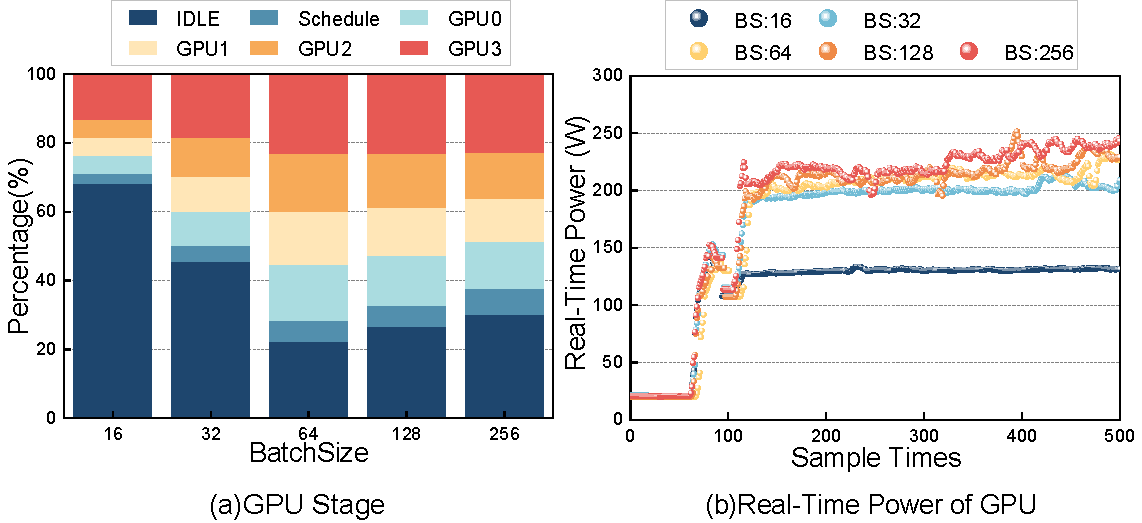
\includegraphics[width=1\linewidth]{figures/lifecycle_power_nq_new.pdf  }
%     \caption{(a) The distribution of the execution time in different stages running on four GPUs. (b) Real-time power usage in a parallel inference with different batch sizes.}
%     \label{fig:lifecyclepower}
% \end{figure}

% \begin{figure}[t]
%     \centering
%     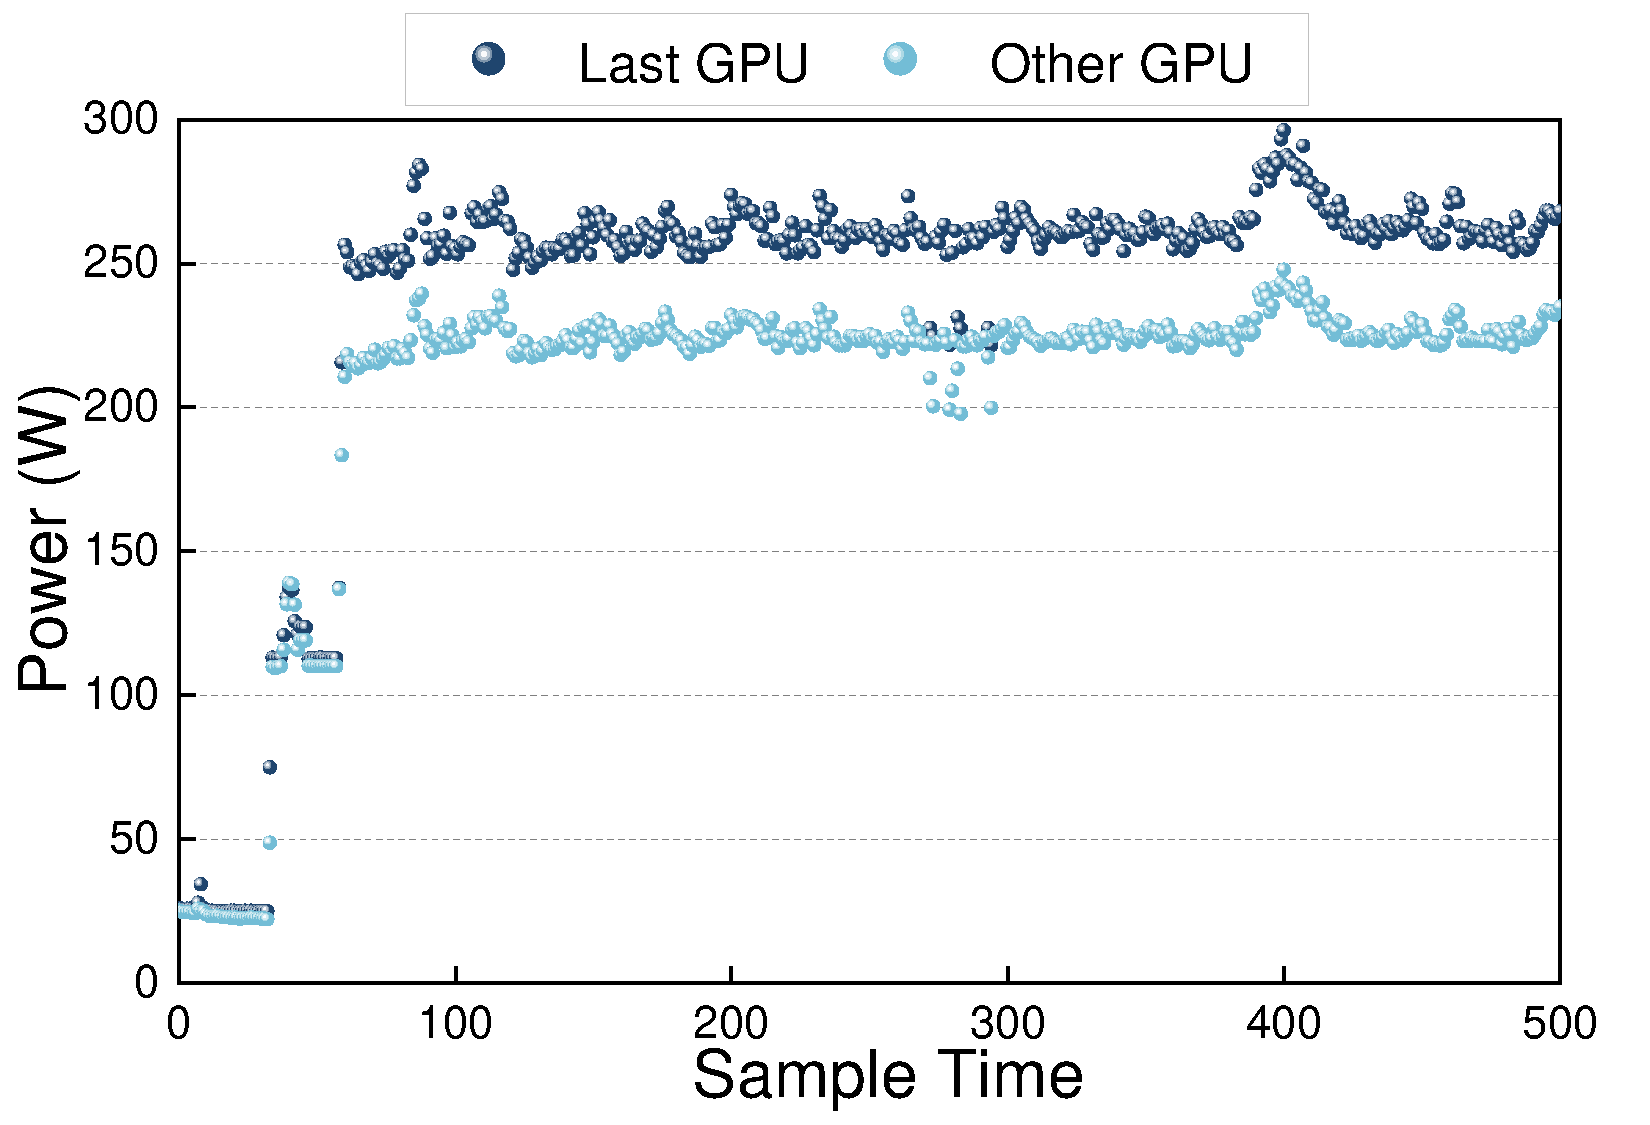
\includegraphics[width=0.9\linewidth]{figures/real_time_power.pdf}
%     \caption{Real-time power usage using the Llama3-8B model with four pipeline stages on RTX 3090 GPUs.}
%     \label{power-runtime}
% \end{figure}

% Figure 5
% \begin{figure}[t]
%     \centering
%     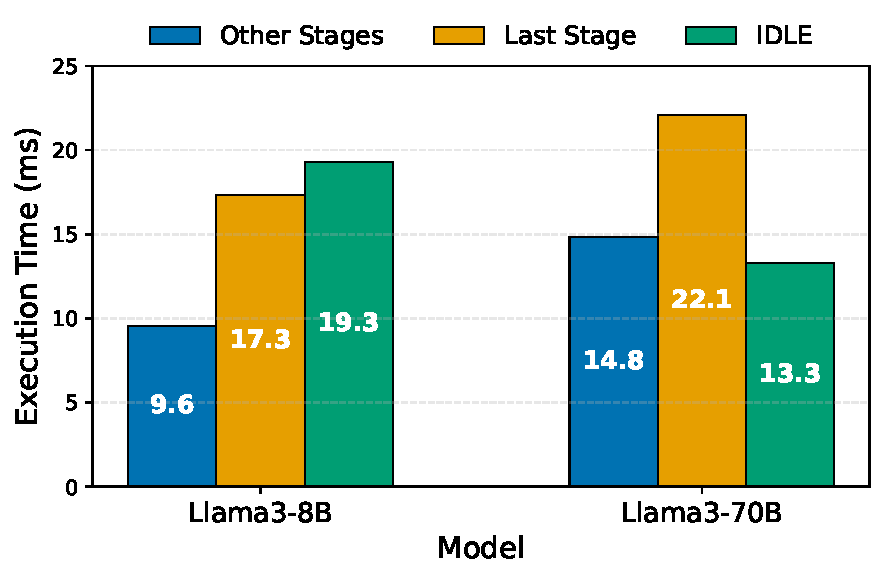
\includegraphics[width=0.9\linewidth]{figures/lifecycle_power_nq_new_new_new_new_new_new_new_new.pdf}
%     % \caption{(a) The distribution of the execution time in different stages. (b) Real-time power usage in a parallel inference for Llama3-8B.}
%     \caption{Execution time across pipeline stages for Llama3-8B and Llama3-70B.}
%     \label{fig:lifecyclepower}
% \end{figure}

% Figure 6
% \begin{figure}[t]
%     \centering
%     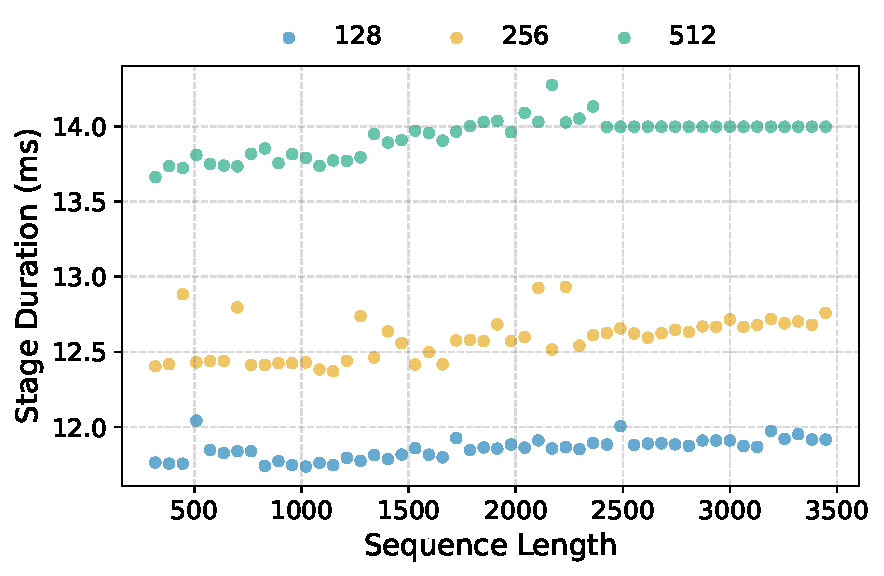
\includegraphics[width=0.9\linewidth]{figures/duration_seqlen_new_new.pdf}
%     \caption{Stage duration of Llama3-70B across different sequence lengths under batch sizes of 128, 256, and 512. Each color corresponds to a distinct batch size configuration.}
%     \label{fig:duration_seqlen}
% \end{figure}

% Figure 5 And 6
\begin{figure}[t]
    \centering
    \begin{minipage}[t]{0.48\textwidth}
        \centering
        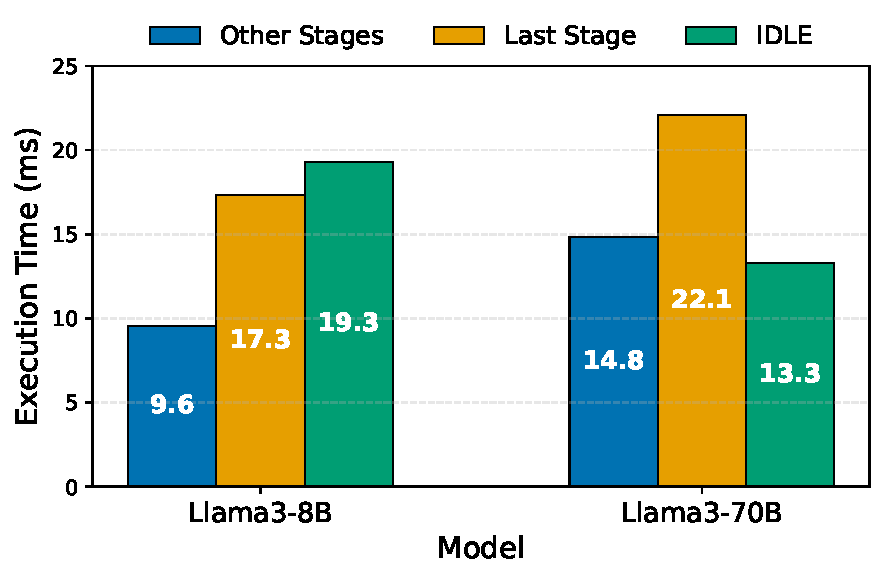
\includegraphics[width=\textwidth]{figures/lifecycle_power_nq_new_new_new_new_new_new_new_new.pdf}
        \caption{\lyzcheck{Execution time across pipeline stages for Llama3-8B and Llama3-70B.(x is model(Llama3-8B, Llama3-70B, \hcwplaceholder{XX}), y is Stage Execution Time. Try to make that other stage + idle = last stage)}}
        \label{fig:lifecyclepower}
    \end{minipage}
    \hspace{0.02\textwidth}
    \begin{minipage}[t]{0.48\textwidth}
        \centering
        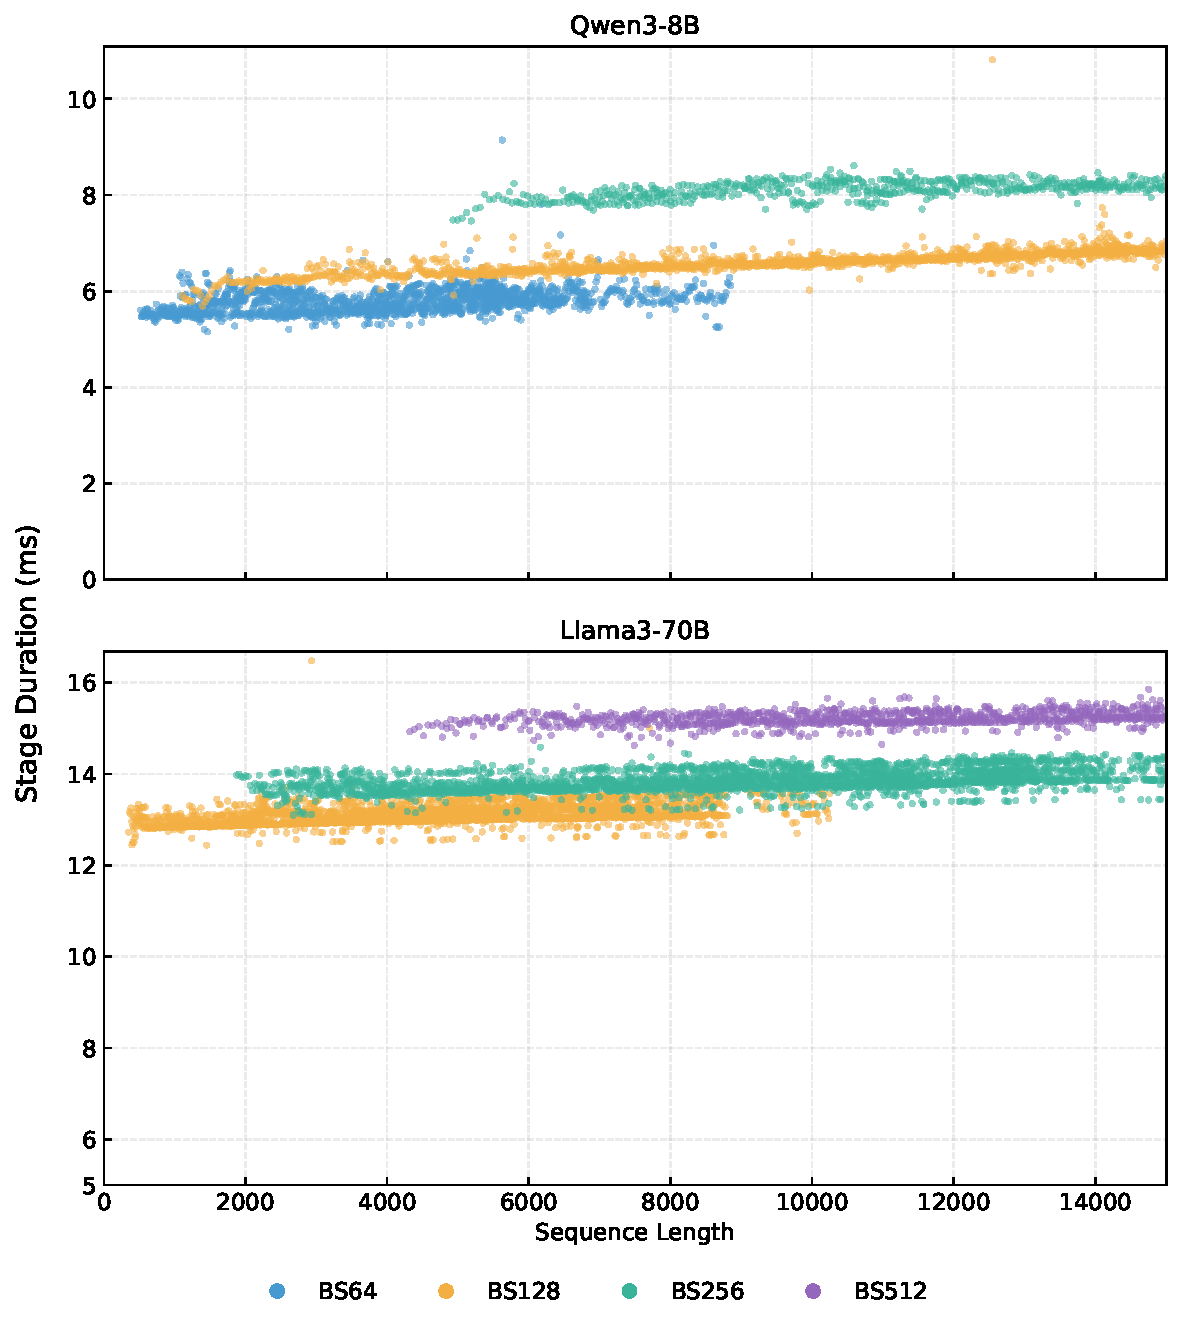
\includegraphics[width=\textwidth]{figures/hcw_final_figures/Fig4_auto_context_main_range_20261017.pdf}
        \caption{\byhcw{Middle-stage decode time versus aggregate batch context length on ShareGPT. Llama3-8B (Sarathi) is above Llama3-70B (SGLang); colors denote batch sizes. Two clipped Llama3-8B timing spikes are marked by triangles.}}
        \label{fig:duration_seqlen}
    \end{minipage}
\end{figure}

%However, the idle state of GPUs does not contribute to energy saving. 
%This leads to unnecessary power consumption, which adversely affects the overall power and energy efficiency of the system.


% \subsection{Execution Time of Stages}
\subsection{Stable Execution Time of Stage}
\label{sec:stableexecutiontime}
% The execution of a batch is stable

% \bygxl{See the comments.}
%每一个推理的任务是由Transformer+PostProcessing构成的
%Transformer的Attention部分和sequence length相关
%同时，各种优化技术【加参考文献】都在优化这一部分，减少sequence length对它的影响
%FFN只和模型相关
%因此，一个request的一个stage的时间，基本上是稳定的
%上例子，说明对于batch固定的时候，sequence length在变化，但是stage execution time是不变的
%另起一段
%同理，按照2.2节的分析，post processing也是不变的
%再起一段
%batch的大小，也就是一个stage中request的数量，会导致stage的时间scale up linearly
%分析原因，因为一个request是一个tensor，一个batch是把tensor合并成了matrics，batchsize就是matricx的行数
%However, 对于不同的batchsize, Ts/Tf是一个稳定的值，以及Ts(p1)/Ts(p0)是一个稳定的值（主要是表达这些东西与batchsize无关），看看
%结论段：虽然每一个调度的Batchsize不同，但因为比例相同，因此给了我们利用power cap调整stage并对齐执行时间的机会

% However, batchsize 是实时变化的by the scheduler to select the input prompts by user which is random.
% 这个random的prompts导致了batchsize符合正态分布，从而导致

According to the analysis in Section~\ref{sec:llmandtransformer}, several factors may influence the execution time of each stage, including \textit{sequence length} and \textit{batch size}.
However, our observations show that \textit{sequence length} has only a limited impact on stage execution time, particularly during the decode phase, which dominates the overall inference cost.




While the computation overhead of the Attention scales linearly with \textit{sequence length}, recent GPU kernels such as FlashDecoding++~\cite{hong2023flashdecoding++} and FlashInfer~\cite{ye2025flashinfer} substantially weaken this dependency by reorganizing memory access (e.g., double-buffered tiling) and introducing block-sparse KV storage.
Moreover, the FFN consistently dominates layer computation—accounting for roughly \hcwplaceholder{XX}--\hcwplaceholder{XX}\% of decode time compared with \hcwplaceholder{XX}--\hcwplaceholder{XX}\% for Attention~\cite{cheng2025ecco}—and its matrix multiplications are independent of sequence length.
Together, the dominance of sequence-independent FFN compute and the efficiency of optimized attention kernels ensure that stage execution time exhibits minimal sensitivity to sequence length in practice.

\byhcw{Using ShareGPT at Auto GPU frequency, we measure the mean middle-stage decode time for Llama3-8B on four RTX 3090 GPUs with Sarathi and Llama3-70B on eight A100 GPUs with SGLang. The horizontal axis in Figure~\ref{fig:duration_seqlen} is the sum of request context lengths in a pure-decode batch. At BS256, the median stage time increases by only 0.38 ms for Llama3-8B and 0.27 ms for Llama3-70B when comparing aggregate context lengths of 5,000--6,000 and 14,000--15,000 tokens.}
Consistent with our findings, prior work reports only a 1.5\% increase when the sequence length grows from 1000 to 4000 tokens~\cite{ye2025flashinfer}.
These results confirm that the impact of \textit{sequence length} on stage execution time is negligible.
Thus, the execution time of a stage can be regarded as stable under a predetermined \textit{batch size} configuration.

% Figure 6
% \begin{figure}[t]
%     \centering
%     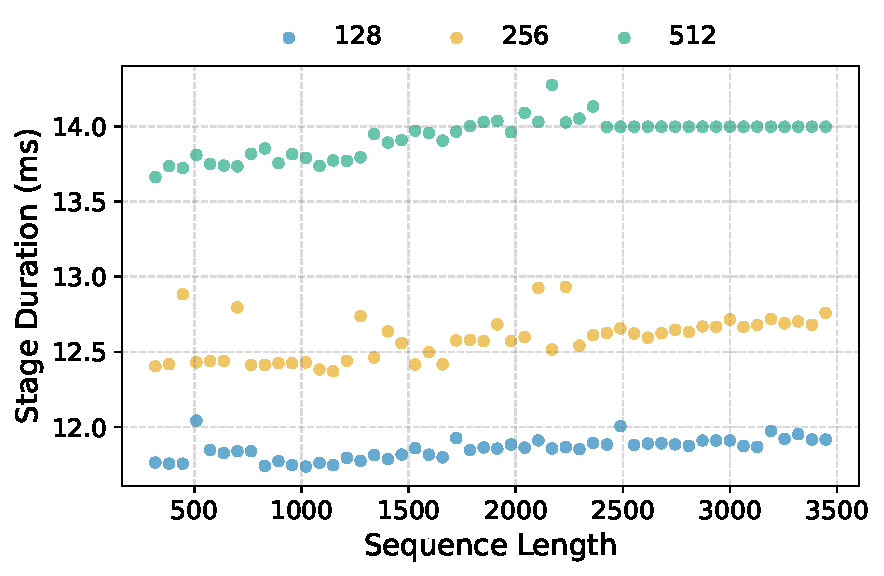
\includegraphics[width=0.9\linewidth]{figures/duration_seqlen_new_new.pdf}
%     \caption{Stage duration of Llama3-70B across different sequence lengths under batch sizes of 128, 256, and 512. Each color corresponds to a distinct batch size configuration.}
%     \label{fig:duration_seqlen}
% \end{figure}




\iffalse
\bylyz{
% Batch size is another factor that may influence stage execution time, as it determines the dimensions of matrices in both Attention and FFN computations. 
% In principle, larger batches lead to more FLOPs due to larger matrix multiplications. 
% Yet, during the decode phase, execution is typically dominated by parameter loading rather than arithmetic throughput. 
% Since model parameters are loaded once per batch regardless of its size, the per-batch execution time remains relatively stable across different batch sizes. 
Batch size is another factor that influences stage execution time. 
Larger batches increase the dimensions of the matrices in both Attention and FFN computations, leading to a theoretical increase in FLOPs. 
Yet during the decode phase, execution is predominantly memory-bound: parameter loading accounts for roughly 70--80\% of total time, while arithmetic operations contribute only 20--30\%~\cite{alizadeh2024llm, recasens2025mind}. 
Since model parameters are loaded once per batch and reused across requests, stage latency remains relatively stable across batch sizes despite the larger matrix operations. 
In practice, batch size cannot be increased arbitrarily because it is constrained by GPU memory capacity. 
For example, prior work reports that a single A100 GPU (40\,GB memory) can accommodate at most 200–300 concurrent sequences of length 1k when serving Llama-65B~\cite{alizadeh2024llm, kwon2023efficient}, and larger batch sizes quickly exceed memory limits. 
These constraints naturally bound the extent to which batch size affects runtime.  
}

\bylyz{
We empirically validate these observations through profiling experiments on eight A100 GPUs using the ShareGPT dataset. 
Here, we define the \textit{global batch size} as the total number of requests processed simultaneously across all running batches. 
Figure~\ref{fig:executiontime_dis} reports the distribution of per-stage latency under different global batch sizes. 
Although small variations exist, the overall latency remains within a narrow range (around 12--14 ms) across global batch sizes of 128, 256, and 512. 
This confirms that stage execution time is largely insensitive to both sequence length and batch size during the decode phase, reinforcing the assumption of runtime stability that underpins our analytical performance model in Section~\ref{sec:profiling}.
}

\begin{figure}[t]
    \centering
    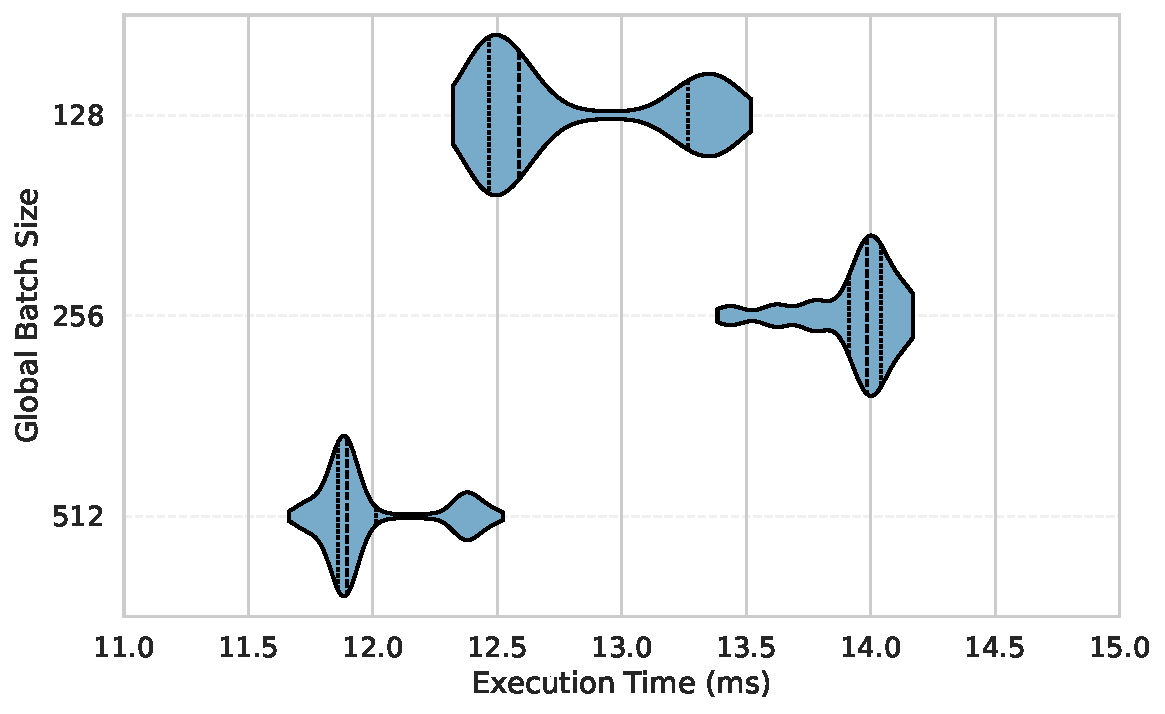
\includegraphics[width=0.9\linewidth]{figures/executiontime_dis.pdf}
    \caption{Distribution of batch execution times across Global Batch Sizes on the ShareGPT dataset using Llama3-70B on eight A100.}
    \label{fig:executiontime_dis}
\end{figure}

\fi



\subsection{GPU Frequency Management}


%1. 现在的GPU是支持电源管理的，但是这个东西根本帮不到我们，因为需要周期
%2. 电源管理的本质是主频的变化，也就是限制能耗会导致计算变慢
%3. 这两个东西之间是有数学关系的，可以是别人的相关研究，也可以是我们的实验
%4. 利用这个数学关系，可以指导我们填上这个气泡

% 现在的GPU可以通过负载自动调节性能状态

% Modern GPUs are equipped with advanced power management capabilities, enabling them to dynamically adjust power and energy consumption in response to varying computational load\cite{nvidia}. 
% Specifically, GPUs support multiple performance states (P-states), each characterized by different levels of power consumption and computational performance\cite{nvidia}. 
% These states allow parameters such as operating frequency and power usage to be tuned to match the demand of the workload, i.e., it will transition from a higher performance state (e.g., P0) to a lower one (e.g., P8).
% Such a dynamic adjustment can optimize the power consumption and achieve a balance between performance and energy efficiency.


\bylyz{
GPU core frequency is a configurable operating parameter that affects both energy efficiency and execution
time. Modern GPUs employ dynamic voltage and frequency scaling (DVFS) to adapt their operating conditions to
workload demands within power and thermal limits. However, these hardware-level policies do not necessarily exploit
the slack available between pipeline stages. Software-directed approaches can complement these policies by selecting
frequencies based on workload measurements or predictions.
However, these pipeline bubbles last only tens of milliseconds, making it challenging to monitor workload changes, select an appropriate frequency, and complete the frequency transition within such a short time window.
}

% \bygpt{
% GPU core frequency is a configurable operating parameter that affects both power consumption and execution time. Modern GPUs employ dynamic voltage and frequency scaling (DVFS) to adapt their operating conditions to workload demands within power and thermal limits. However, these hardware-level policies do not necessarily exploit the slack available between pipeline stages. Software-directed approaches can complement these policies by selecting frequencies based on workload measurements or predictions. For pipeline bubbles lasting only tens of milliseconds, workload monitoring, control decisions, and frequency transitions must be coordinated within short time windows. Their overheads depend on the GPU platform and control interface and can limit the benefits of adjusting frequencies in response to individual bubbles.
% }

% \bygemini{
% Frequency is a critical and configurable parameter in modern GPUs that directly influences both power consumption and computation latency. Although modern GPUs can dynamically adjust their frequency to reduce power based on workload fluctuations, relying solely on such automated mechanisms is typically insufficient because these adjustments lack adequate accuracy. Consequently, existing studies often focus on manually setting precise frequencies by capturing and predicting workload variations. However, these manual adjustments usually operate at a granularity of seconds or longer, whereas pipeline bubbles frequently last for only tens of milliseconds. Such brief durations make it extremely challenging for GPUs to accurately detect workload shifts and apply appropriate frequency configurations in a timely manner.
% }


% Extensive research has been conducted on the dynamic power management of GPUs\cite{wang2021dynamic, bridges2016understanding, mercati2017multi, krzywaniak2023dynamic}. 
% Generally, the adjustment process relies on the workload traces to regulate the power states at a granularity level of seconds or longer\cite{chen2023joss, singhania2024methodology}. 
% However, in an LLM inference, pipeline bubbles often last only tens of milliseconds. 
% Such short periods make it challenging for GPUs to accurately detect workload changes and adjust their power states accordingly.
% \bygxl{Not sure if correct. Change it when necessary.}



%The fine-grained time scale further complicates manual adjustments to the GPU power state in response to rapidly changing demands. As a result, existing solutions are inadequat e for achieving dynamic power adjustments during runtime to accommodate fluctuating computational needs.Therefore, it is difficult for existing technical methods to achieve dynamic power adjustment at runtime to adapt to changing computing tasks. 


%Although the GPU's automatic power management does not effectively address the energy consumption issues caused by pipeline bubbles, it has led us to an important insight. We identified that the core of power management lies in adjusting the GPU's power, controlling energy consumption by modifying power levels, and adapting computational capacity to meet varying load demands. Through experimental analysis, this paper reveals a mathematical relationship between power and program performance. This finding offers a new approach: by adjusting the GPU's power, we can manipulate its computation time, effectively filling pipeline bubbles and optimizing overall energy efficiency.

\section{The \thisproj{} Framework}
\label{sec:design}


\subsection{The Design}
\label{Principle Model}

\begin{figure}[t]
    \centering
    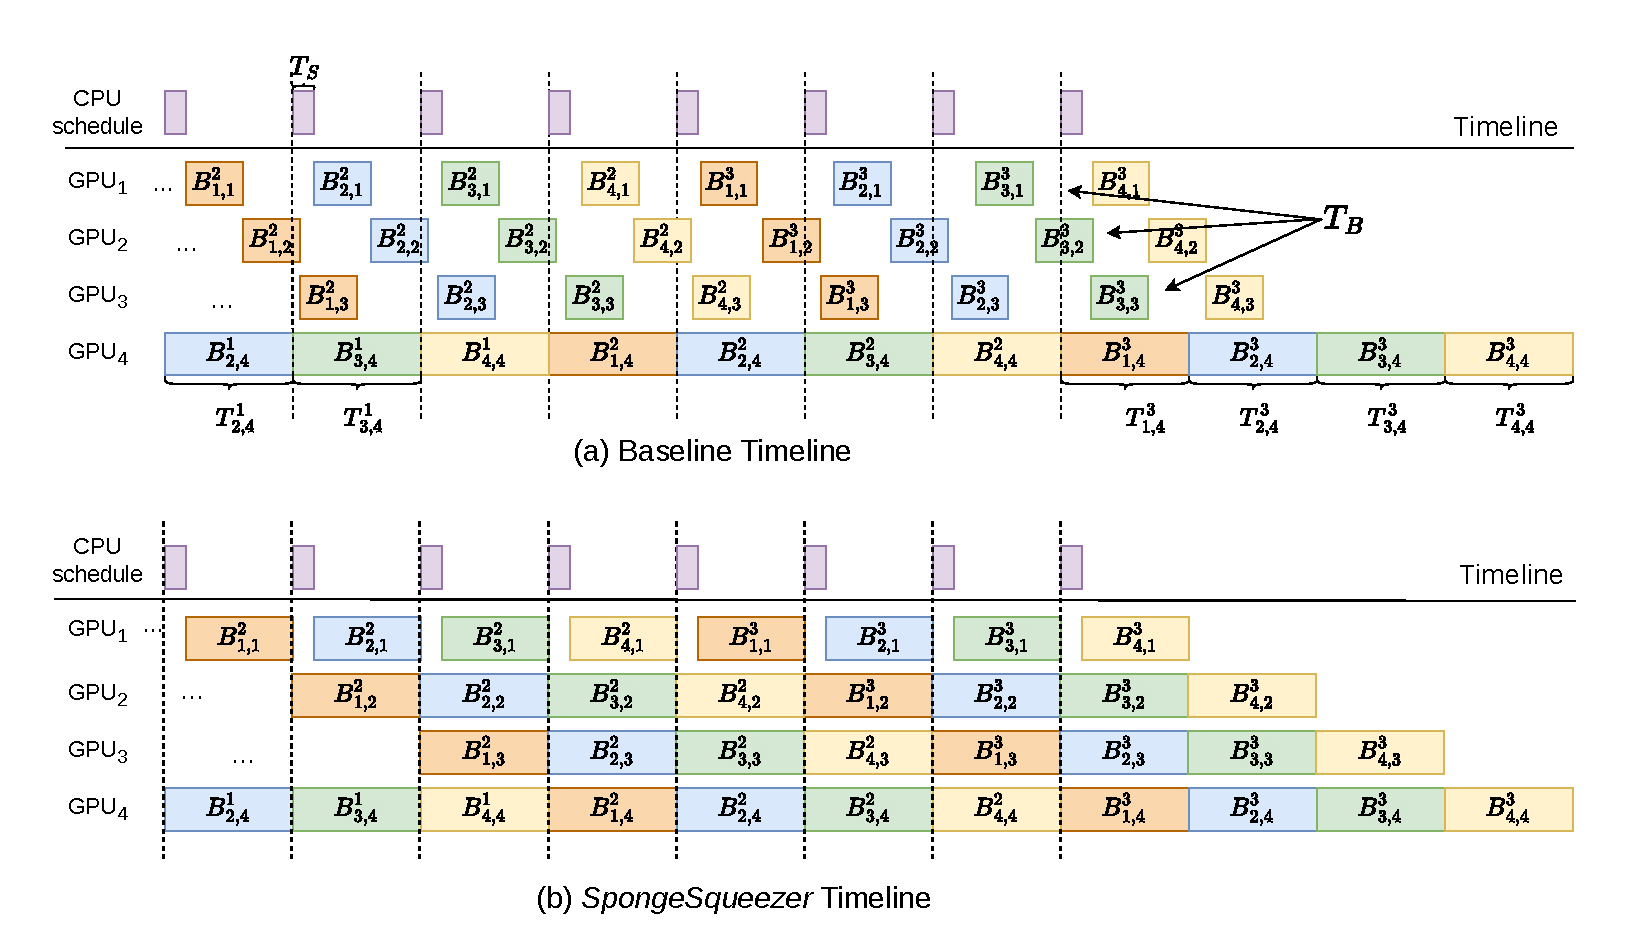
\includegraphics[width=0.9\linewidth]{figures/TACO_Rebuttal/timeline.pdf}
    \caption{(a) The timeline that shows pipeline bubbles in Continuous Batching. (b) The time line that shows \thisproj{} can reduce pipeline bubbles by aligning the stages through frequency adjustment with minimal impact on performance.}
    \label{timeline}
\end{figure}
We ignore the Prefill phase and focus only on the Decode phase, which is the main part of the inference process where pipeline bubbles become unavoidable due to the limited GPU memory capacity.
%To better analyze this phenomenon, 
We extract the part of Decode phase from Figure~\ref{workflow} and show it in Figure~\ref{timeline}(a). 

% We define the process time of an iteration in the batch $i$ on $GPU_j$ (i.e. in stage $j$) as $T_{i,j}$ (see Figure \ref{timeline}(a)).
% For instance, the execution time of any iteration in batch $B_2$ on $GPU_3$, represented by the blue block in the last row, is denoted as $T_{2,3}$.
% The execution time of the scheduler on the CPU side is marked as $T_S$ and depicted as the purple blocks in the first row of the figure. 
% Additionally, we represent the time consumed by pipeline bubbles as $T_B$, which corresponds to the blank areas in the pipeline. 
\bylyz{
We define the processing time of batch $B_{i,j}^{k}$ as $T_{i,j}^{k}$, representing the execution time of batch $i$ on $\text{GPU}_j$ during the $k$-th iteration (see Figure \ref{timeline}(a)).
Let $M$ denote the total number of batches, $N$ the number of GPUs, and $K$ the total number of iterations.
The indices are bounded as follows: $1 \leq i \leq M$, $1 \leq j \leq N$, and $1 \leq k \leq K$.
Additional, the execution time of the scheduler on the CPU side is marked as $T_S$ and depicted as the purple blocks in the first row of the figure. 
We also represent the time consumed by pipeline bubbles as $T_B$, which corresponds to the blank areas in the pipeline. 
}

% An imbalance can be observed in the pipeline stages with the last stage taking significantly longer time than the others. 
% Experimental results indicate that the execution time for all $T_{i,1}$ to $T_{i,n-1}$ is almost the same, while the last stage $T_{i,n}$ is significantly longer, reaching nearly twice that of the earlier stages in the Llama3-8B.
% Consequently, only the last stage of the pipeline remains fully occupied, and the system’s end-to-end latency can be approximated as the cumulative execution time of all batches on $GPU_n$, expressed as:$\sum_{i=1}^{EOS}T_{i,n}$.
% And the bubbles occupy a substantial portion of the total pipeline execution time.
% Specifically, the ratio of the total bubble time to the total execution time is: $$\frac{T_B}{\sum_{i=1}^{EOS}\sum_{j=1}^NT_{i,j}}$$ 

\bylyz{
An imbalance can be observed in the pipeline stages with the last stage taking significantly longer time than the others. 
Experimental results indicate that the execution time for all $T_{i,1}^{k}$ to $T_{i,N-1}^{k}$ is almost the same, while the last stage $T_{i,N}^{k}$ is significantly longer, reaching nearly twice that of the earlier stages in the Llama3-8B.
Consequently, only the last stage of the pipeline remains fully occupied, and the system’s end-to-end inference time can be approximated as the cumulative execution time of all batches on GPU$_N$, expressed as:$\sum_{i=1}^{M}\sum_{k=1}^{EOS}T_{i,N}^{k}$.
And the bubbles occupy a substantial portion of the total pipeline execution time.
Specifically, the ratio of the total bubble time to the total execution time is: $$\frac{\sum{T_B}}{\sum_{i=1}^{M}\sum_{j=1}^{N}\sum_{k=1}^{K}T_{i,j}^{k}}$$ 
}



% T_{i,j} (j=0,...,N-1)
To address this issue, we propose \thisproj{}, a solution that leverages the frequency scaling technology to extend $T_{i,j}^{k}$ by scaling down GPU frequency, thereby lengthening the execution time to fill the bubble time $T_B$. 
%Because individual pipeline bubbles are short-lived and arise from rapid load fluctuations, real-time dynamic adjustments are ineffective at capturing and mitigating them. 
%Instead, \thisproj{} employs a static power adjustment strategy by setting a fixed power limit.
As illustrated in Figure~\ref{timeline}(b), the optimized timeline demonstrates the improvements achieved through this approach. \thisproj{} minimizes pipeline bubbles by aligning the execution time $T_{i,j}^{k}$ across all GPUs to match $T_{i,N}^{k}$. 
Ideally, this adjustment creates a balanced pipeline where every stage has a duration equal to $T_{i,N}^{k}$.
It is important to note that GPU$_1$ must wait for the scheduler to assemble the batch, which adds $T_S$ to the execution time of stage 1.
Consequently, the execution time for the stage on GPU$_1$ is slightly shorter than that of the other GPUs. 
Additionally, as described earlier that the last stage GPU (GPU$_N$) needs to handle other critical tasks, its execution time will directly impact the overall end-to-end inference time. 
To preserve the stability of these critical tasks, \thisproj{} does not adjust the frequency of GPU$_N$.

% There are several techniques to regulate the power thereby adjust the execution time $T_{i,j}^{k}$. 
% These include adjusting the compute core frequency, memory frequency, and the power cap of GPUs. 
% Among them, adjusting the GPU power cap is the simplest approach as it directly limits the GPU's maximum power consumption, which in turn can regulate its performance. 
% The GPU can automatically select the most appropriate power state (p-state) based on the workload to optimize the power/energy efficiency without compromising the performance.

\bylyz{
Modern GPUs provide interfaces to set both maximum and minimum frequency constraints.
In our approach, we configure the maximum and minimum constraints to the exact same value, thereby forcing the GPU to run at a fixed frequency. 
This guarantees that all batches execute under a uniform frequency and mitigates the impact of frequency-induced fluctuations on the stability of stage execution time.
}

% \bygpt{
% On supported GPUs, software interfaces allow the lower and upper bounds of the core frequency to be configured. We set both bounds to the same supported value to request a fixed core frequency. Maintaining this setting across batches on a given GPU helps reduce frequency-induced variation in stage execution time, although the achieved frequency may still be affected by power and thermal limits.
% }

% \bygemini{
% Modern GPUs provide interfaces to set both maximum and minimum frequency constraints. In our approach, we configure the maximum and minimum constraints to the exact same value, thereby forcing the GPU to run at a fixed frequency. This guarantees that all batches execute under a uniform frequency and mitigates the impact of frequency variations on the stability of stage execution times.
% }

% % Figure 8
% \begin{figure}[t]
%     \centering
%     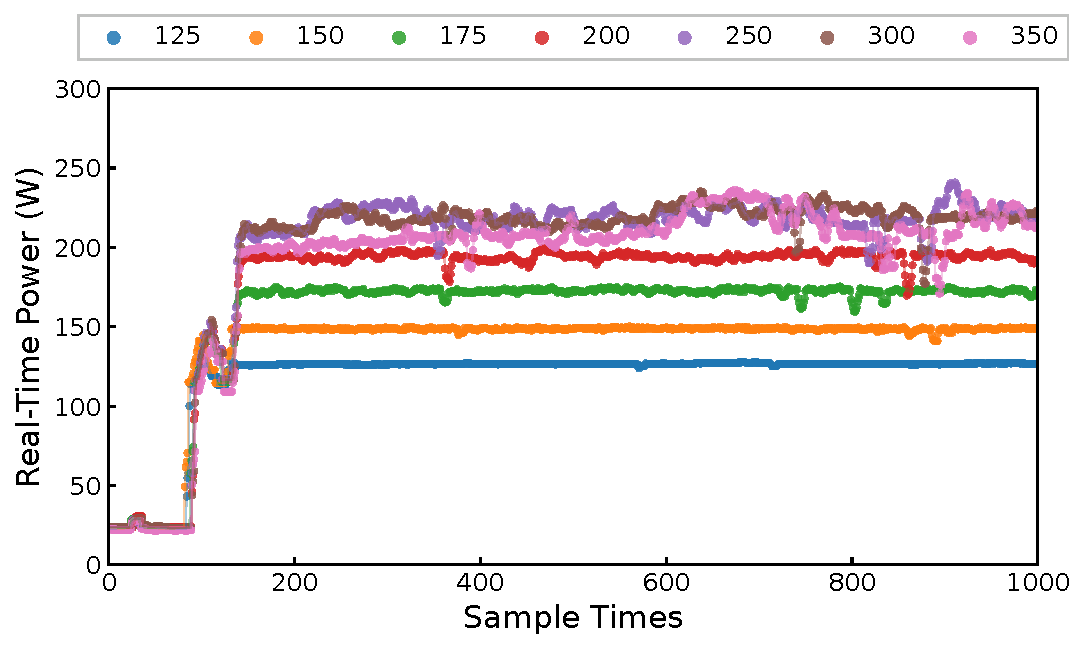
\includegraphics[width=0.8\linewidth]{figures/power_nq_lyz_new_new.pdf}
%     \caption{Real-time power consumption on the Natural Questions dataset using the Llama3-8B model on an RTX 3090 GPU. Different colors represent different GPU power cap settings.}
%     \label{power-runtime}
% \end{figure}

% % Figure 9
% \begin{figure}[t]
%     \centering
%     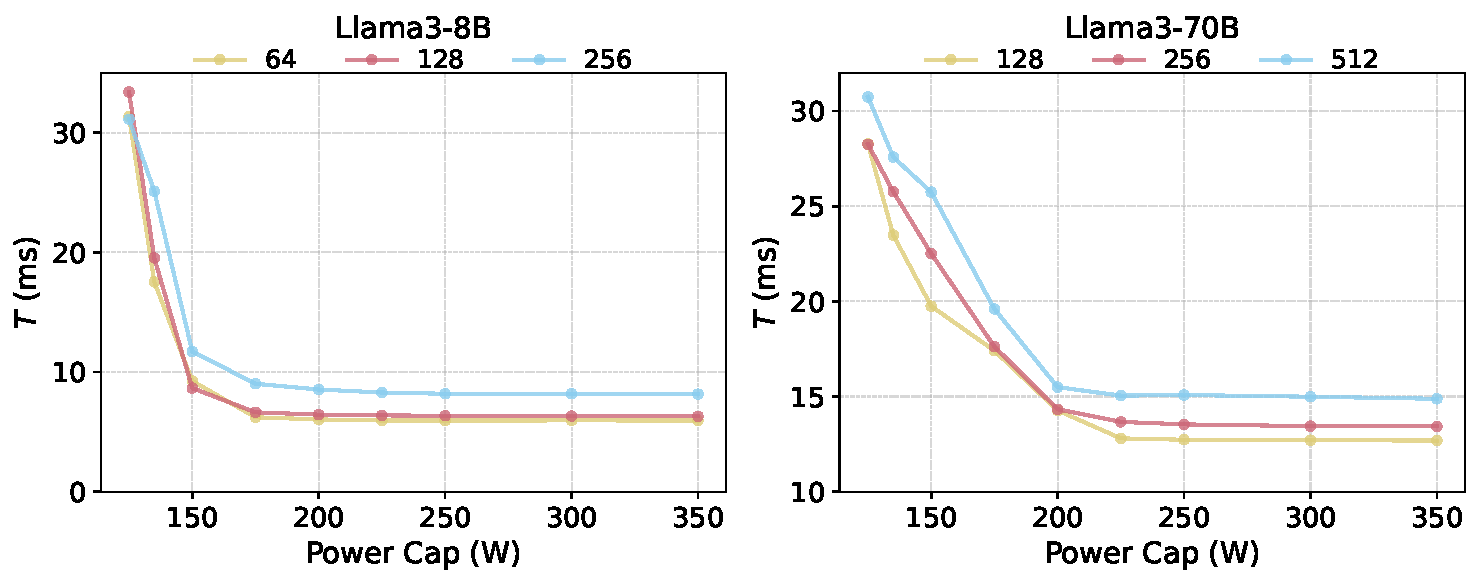
\includegraphics[width=1\linewidth]{figures/execution_time_sampling_new_new.pdf}
%     \caption{Variation of $T$ with different batch size across four Nvidia RTX 3090 GPUs and one NVidia A100 GPU, using Llama3-8B and Llama3-70B on the ShareGPT dataset.}
%     \label{profile_data}
% \end{figure}

% Figure 8 and 9
\begin{figure}[t]
    \centering
    \begin{minipage}[t]{0.48\textwidth}
        \centering
        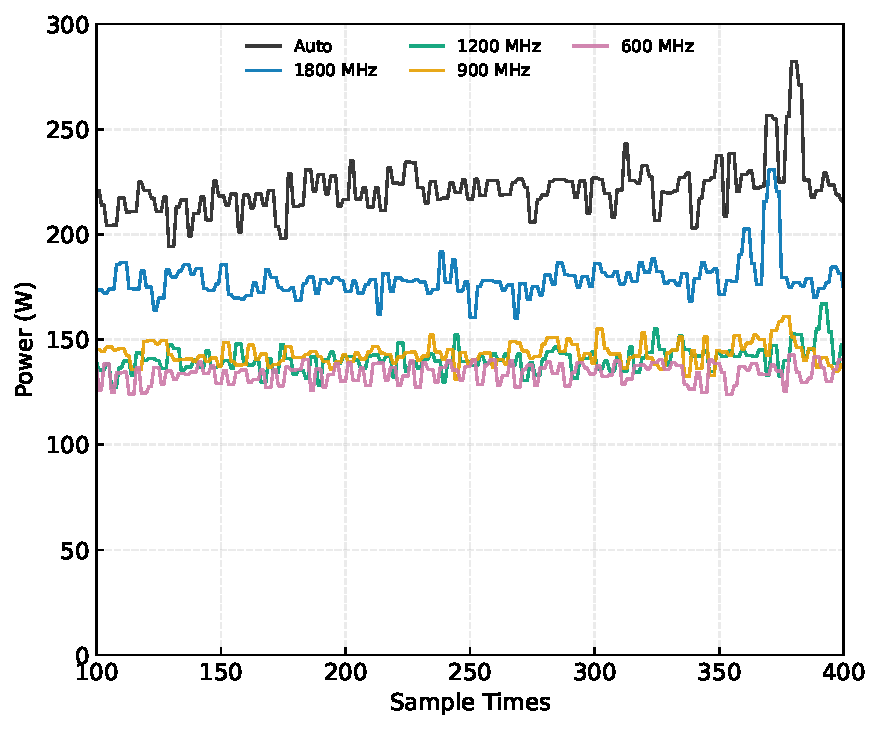
\includegraphics[width=\textwidth]{figures/hcw_final_figures/Fig6_power_sarathi_20261017.pdf}
        \caption{\lyzcheck{Real-time power consumption during inference under various GPU frequency constraints. Different colors represent distinct GPU frequency settings.}}
        \label{power-runtime}
    \end{minipage}
    \hspace{0.02\textwidth}
    \begin{minipage}[t]{0.48\textwidth}
        \centering
        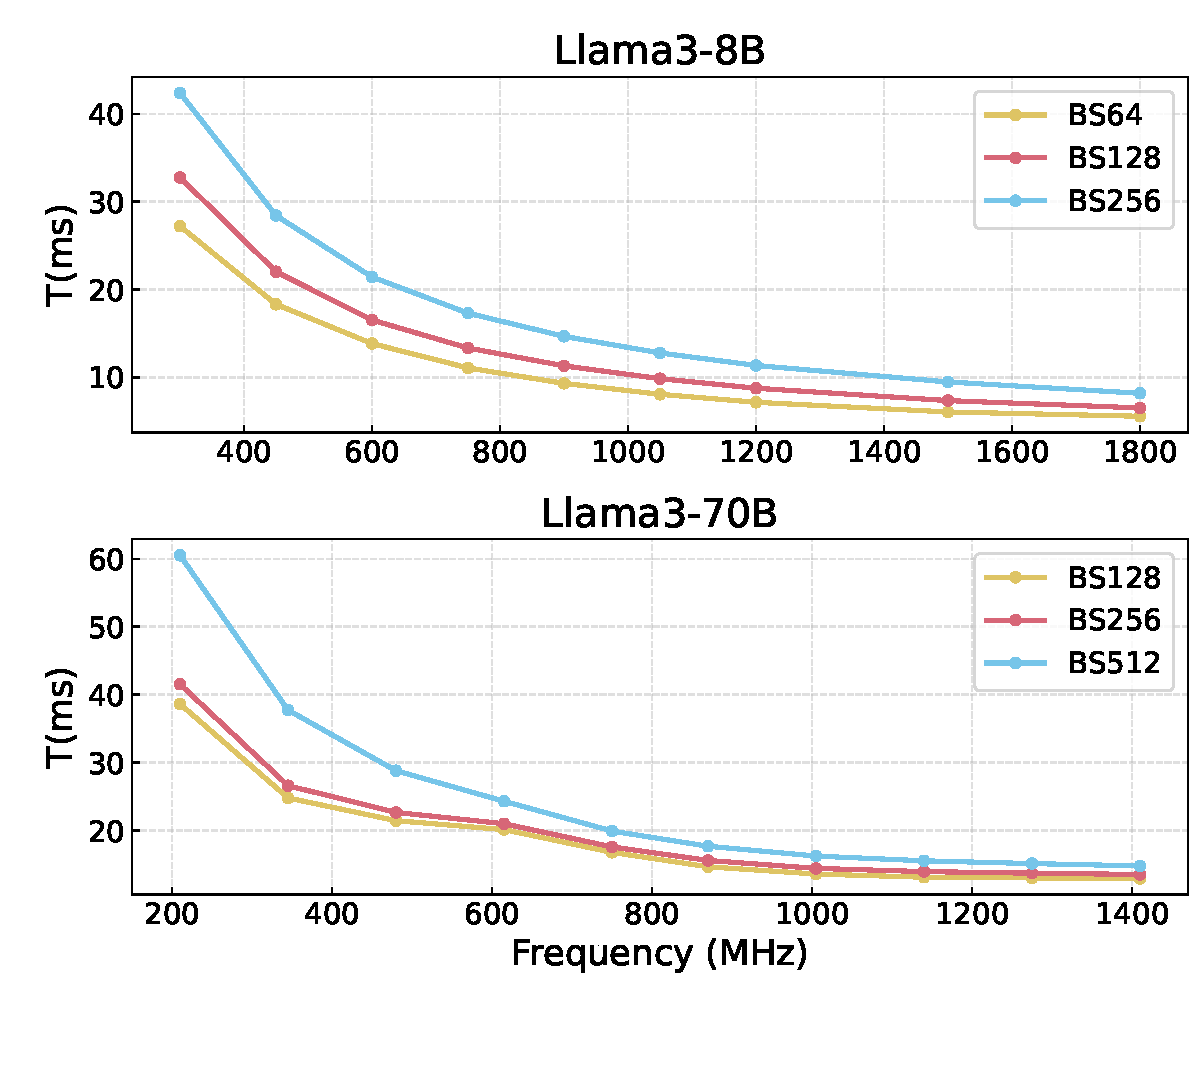
\includegraphics[width=\textwidth]{figures/hcw_final_figures/Fig7_frequency_stage_time_llama_sharegpt_20261018.pdf}
        \caption{\lyzcheck{Variation of $T$ with different batch size across four Nvidia RTX 3090 GPUs and eight Nvidia A100 GPUs, using Llama3-8B and Llama3-70B on the ShareGPT dataset.(The x is $f$, y is $T$. The scatter is the sampled data about $f$ and $T$. Use the line to connect these scatters.)}}
        \label{profile_data}
    \end{minipage}
\end{figure}

% % Figure 8 And 9
% \begin{figure}[t]
%     \centering
%     \begin{minipage}{0.48\textwidth}
%         \centering
%         \raisebox{-\totalheight}{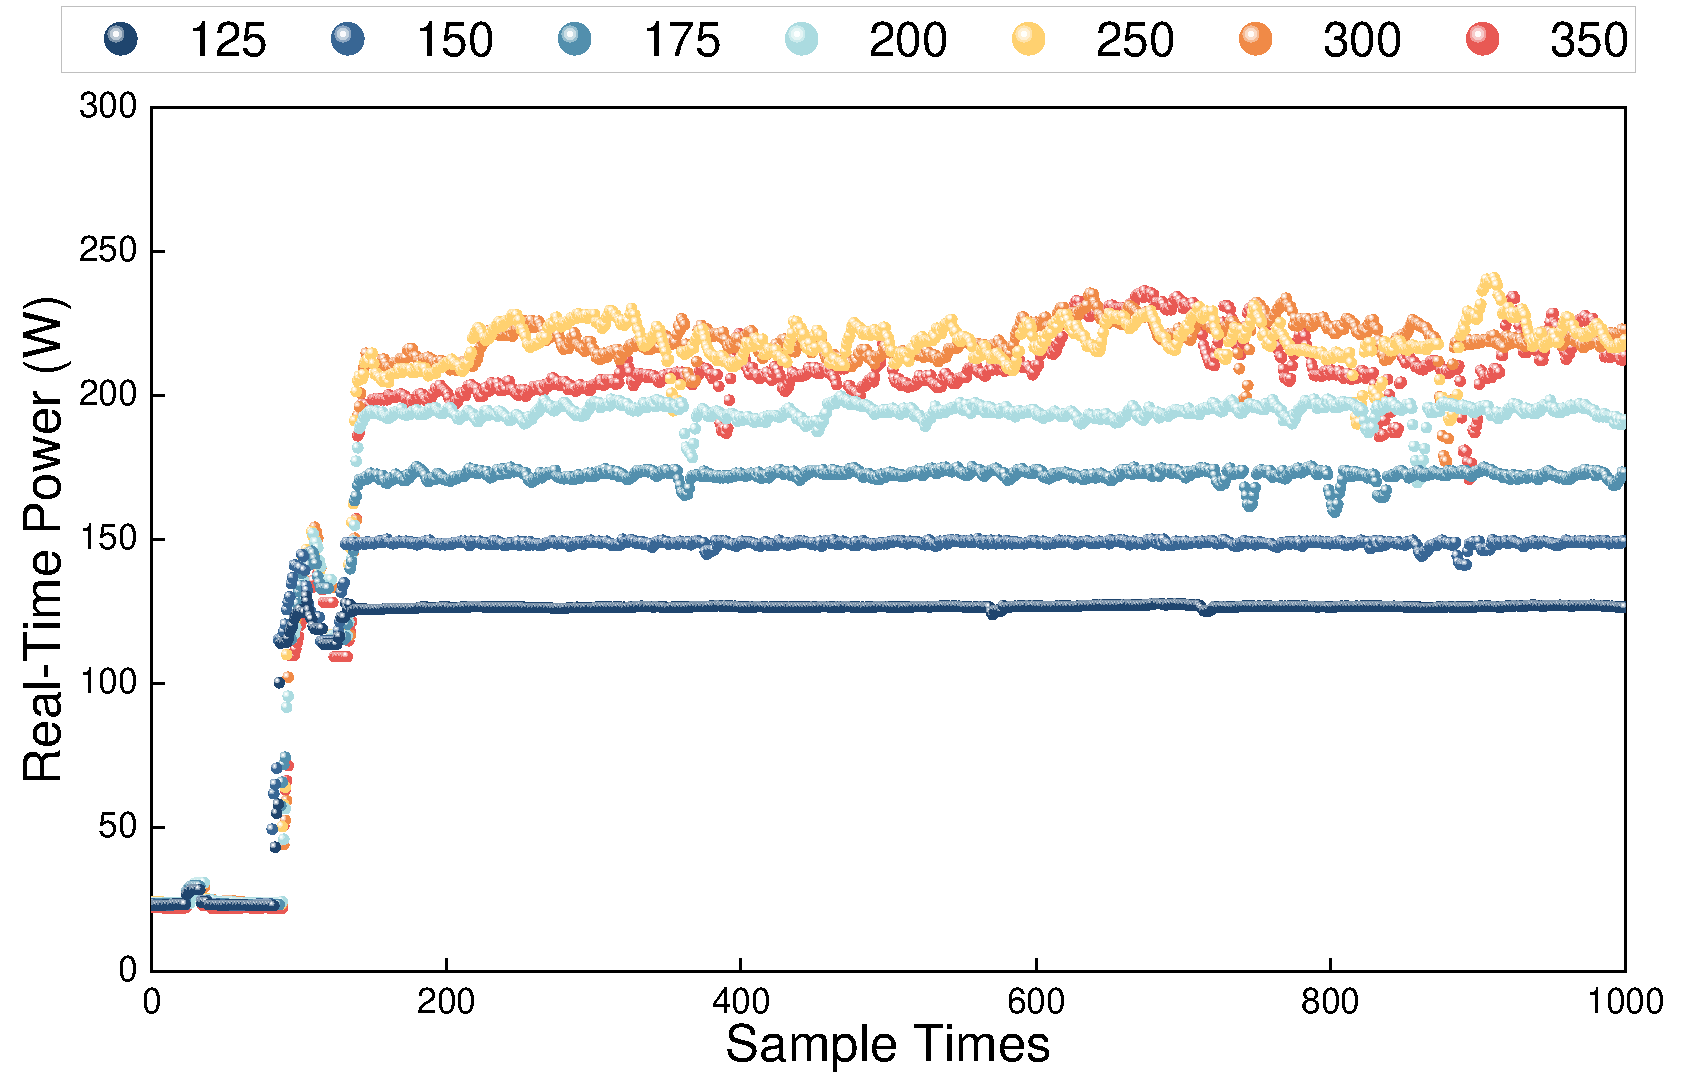
\includegraphics[width=\textwidth]{figures/power_nq_lyz_new.pdf}}
%         \caption{Real-time power consumption on the Natural Questions dataset using the Llama3-8B model on an RTX 3090 GPU. Different colors represent different GPU power cap settings.}
%         \label{power-runtime}
%     \end{minipage}\hfill
%     \begin{minipage}{0.48\textwidth}
%         \centering
%         \raisebox{-\totalheight}{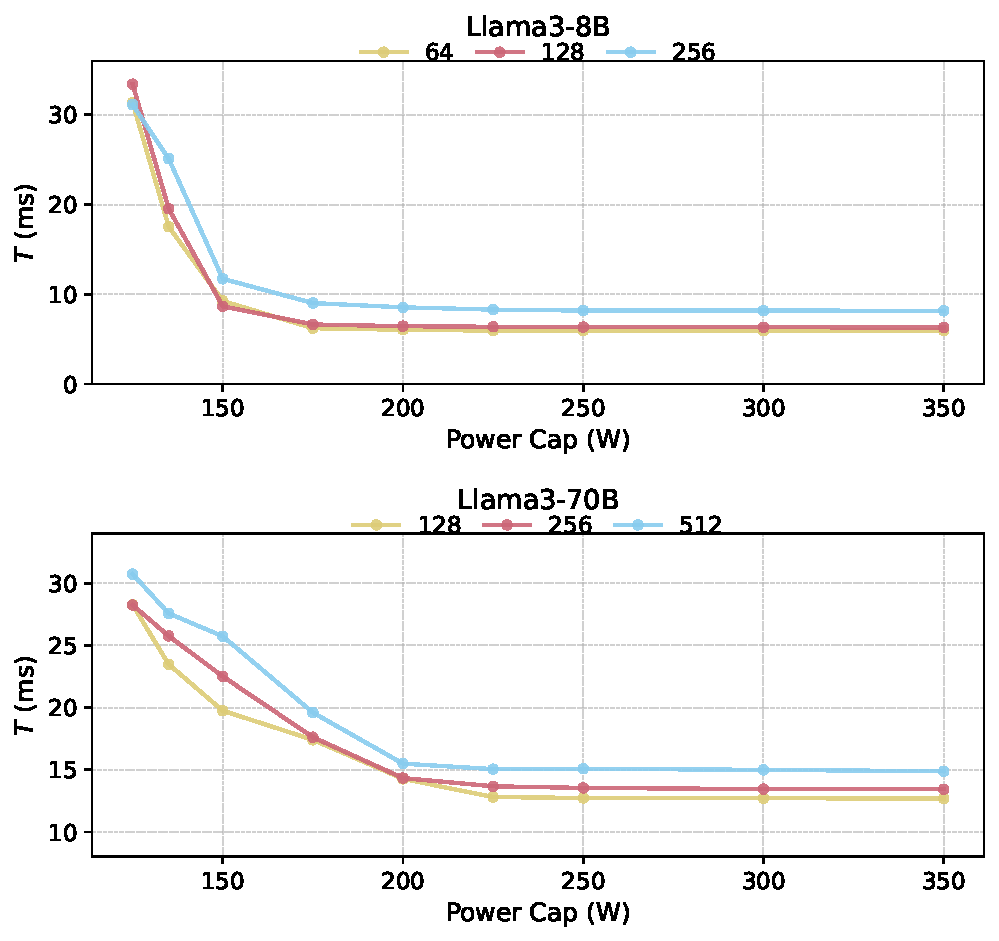
\includegraphics[width=\textwidth]{figures/execution_time_sampling_new_new_new_new.pdf}}
%         \caption{Variation of $T$ with different batch size across four Nvidia RTX 3090 GPUs and one NVidia A100 GPU, using Llama3-8B and Llama3-70B on the ShareGPT dataset.}
%         \label{profile_data}
%     \end{minipage}
% \end{figure}

% \begin{figure}
% 	\centering
% 	\begin{minipage}[t]{\linewidth}
% 		\centering
% 		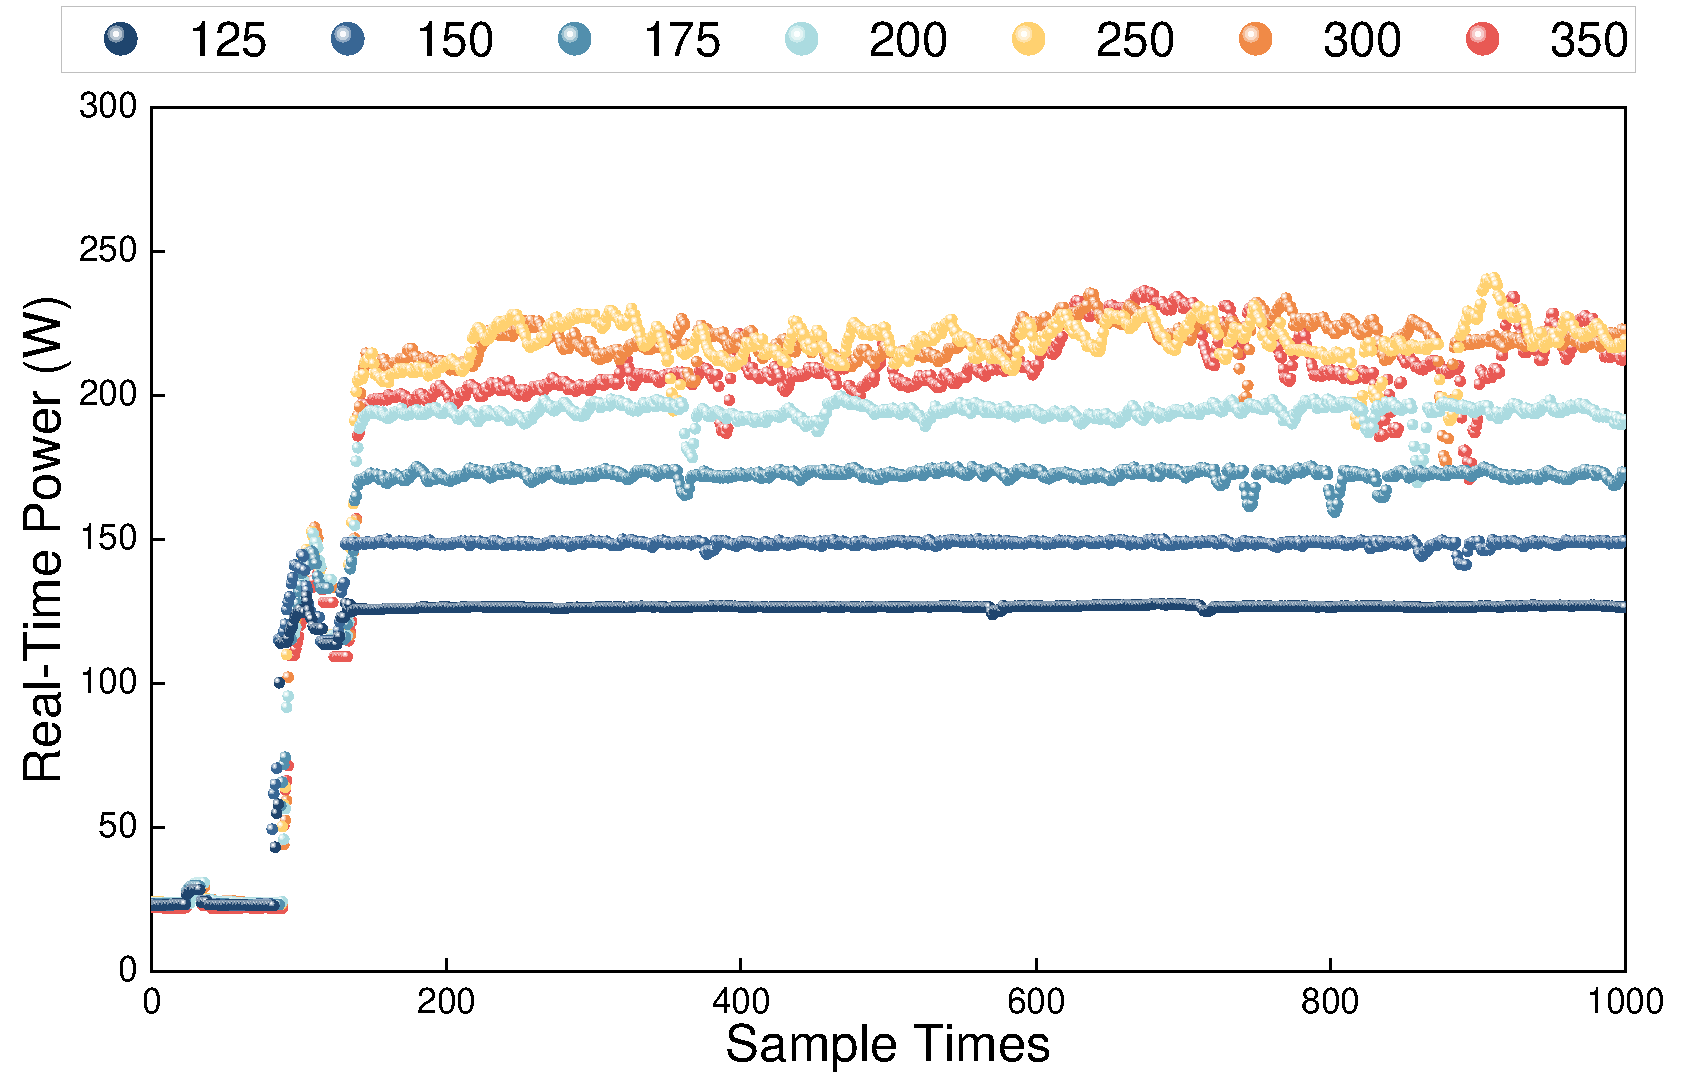
\includegraphics[width=3.3in]{figures/power_nq_lyz_new.pdf}
% 		\caption{Real-time power consumption on the Natural Questions dataset using the Llama3-8B model on an RTX 3090 GPU. Different colors represent different GPU power cap settings.}
% 		\label{power-runtime}
% 	\end{minipage}
% 	\begin{minipage}[t]{\linewidth}
% 		\centering
% 		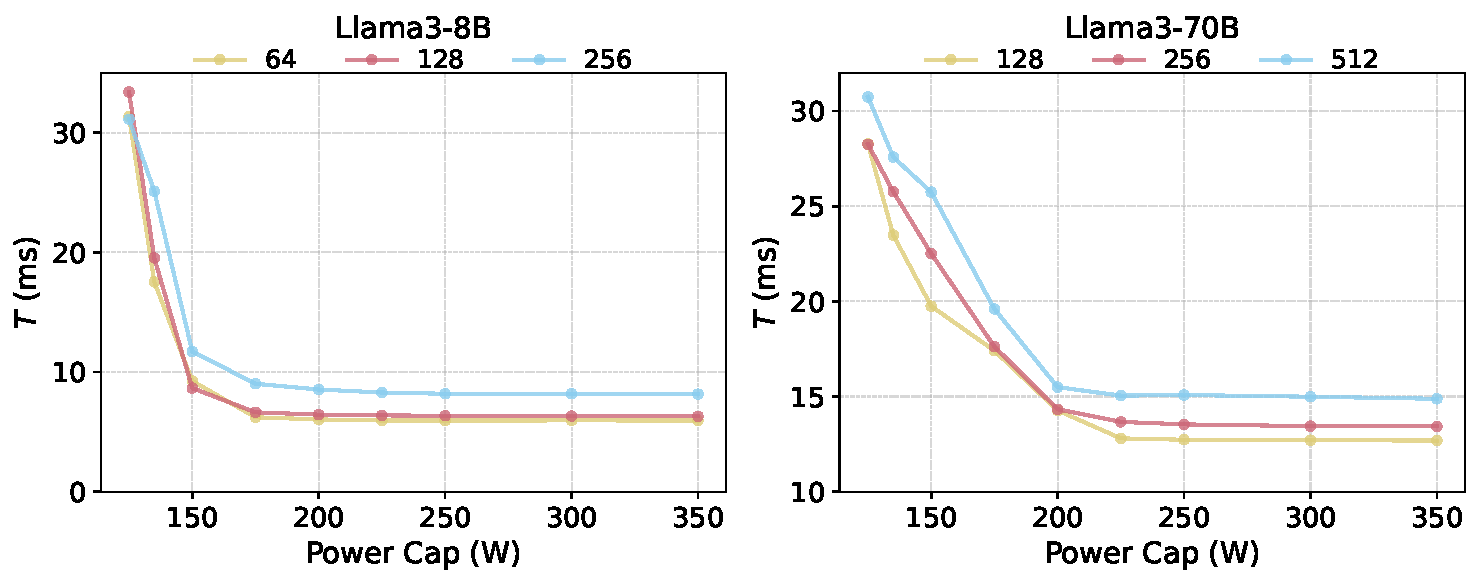
\includegraphics[width=3.3in]{figures/execution_time_sampling_new_new.pdf}
% 		\caption{Variation of $T$ with different batch size across four Nvidia RTX 3090 GPUs and one NVidia A100 GPU, using Llama3-8B and Llama3-70B on the ShareGPT dataset.}
% 		\label{profile_data}
% 	\end{minipage}
%     \label{LLM architecture}
% \end{figure}

% Figure~\ref{power-runtime} illustrates the impact of the power cap on real-time power by sampling actual power consumption during online inference.
% The data is collected during inferences of the Llama3-8B model on RTX 3090 GPUs.
% The results show that the power cap setting operates independently of the DVFS mechanism. 
% By configuring the power cap, the GPU's DVFS mechanism continues to dynamically adjust real-time power based on workload demands.
% At the start of inference, power consumption is relatively low. As the workload increases, power consumption rises significantly while fluctuating slightly within the defined power cap.
% This demonstrates that setting a power cap effectively limits total power consumption without interfering with the normal operation of GPU DVFS, thereby simplifying the design and implementation of \thisproj{}.

\bylyz{
The frequency setting can affect the running power directly.
Figure~\ref{} illustrates the impact of the frequency setting on real-time power by sampling actual power consumption during online inference.
The data is collected during inferences of the Llama3-8B model on RTX 3090 GPUs.
The results show that power consumption follows the same trend as frequency, where a lower frequency typically leads to reduced power. 
Given that total energy consumption equals average power multiplied by execution time—and that the execution time remains unchanged because it is determined by the critical path of the last stage whose frequency is left unadjusted—appropriately lowering the frequency can directly decrease overall energy consumption by reducing average power.
}

% \bygpt{
% GPU core frequency directly affects power consumption. \lyzcheck{Figure~\ref{power-runtime} shows GPU power sampled during online inference with Llama3-8B on NVIDIA RTX 3090 GPUs under different frequency settings. The measurements indicate that lower frequencies generally reduce GPU power consumption.} Total GPU energy consumption equals the aggregate average GPU power multiplied by the workload completion time. We keep the last stage's frequency unchanged and lower the frequencies of non-critical stages. If their additional execution time fits within the available pipeline slack without delaying the last stage, the last stage can remain the bottleneck and workload completion time can remain approximately unchanged. Appropriately chosen lower frequencies can therefore reduce total GPU energy consumption by lowering average power.
% }

% \bygemini{
% The frequency configuration directly dictates the operating power. Figure~\ref{fig:power_trace} illustrates the impact of frequency settings on real-time power by sampling actual power consumption during online inference. These measurements were collected while executing the Llama3-8B model on RTX 3090 GPUs. The results show that power consumption follows the same trend as frequency, where a lower frequency typically leads to reduced power. Given that total energy consumption is defined as the product of power and execution time—and that the inference execution time remains unchanged because it is determined by the critical path of the last stage (whose frequency is left unadjusted)—lowering the frequency appropriately directly decreases overall energy consumption.
% }



\subsection{Profiling and Modeling}
\label{sec:profiling}


Precise GPU frequency adjustment is critical in maintaining stable system throughput. 
%If the power limit is set too high, pipeline bubbles may still occur during this period. 
%Conversely, setting the power limit too low could significantly increase $T_{i,j}$, leading to a sharp rise in inference time.
It requires a good understanding of how the frequency $f$ influences the stage time $T_{i,j}^{k}$. 
%这个地方就不要叫power setting了，应该是前面那一段里写出来的那个能耗上限对应的词
However, the complex and dynamic nature of hardware performance makes it challenging to derive an accurate theoretical model. 
Fortunately, through in-depth analysis, we have found that the relationship between $f$ and $T_{i,j}^{k}$ can be fitted. 
%There exists a certain mathematical relationship between the two. 
To accurately quantify this relationship, 
we use a data-driven approach to create an analytical model that describes the relationship between $f$ and $T_{i,j}^{k}$ under various frequency settings through profiling.
%\thisproj{} leverages a data-driven approach by empirical sampling data to create an analytical model the mathematical relationship between a GPU's power cap and $T_{i,j}$ under various power limit configurations. 
% batch 和 T的关系


% Figure 9
% \begin{figure}[t]
%     \centering
%     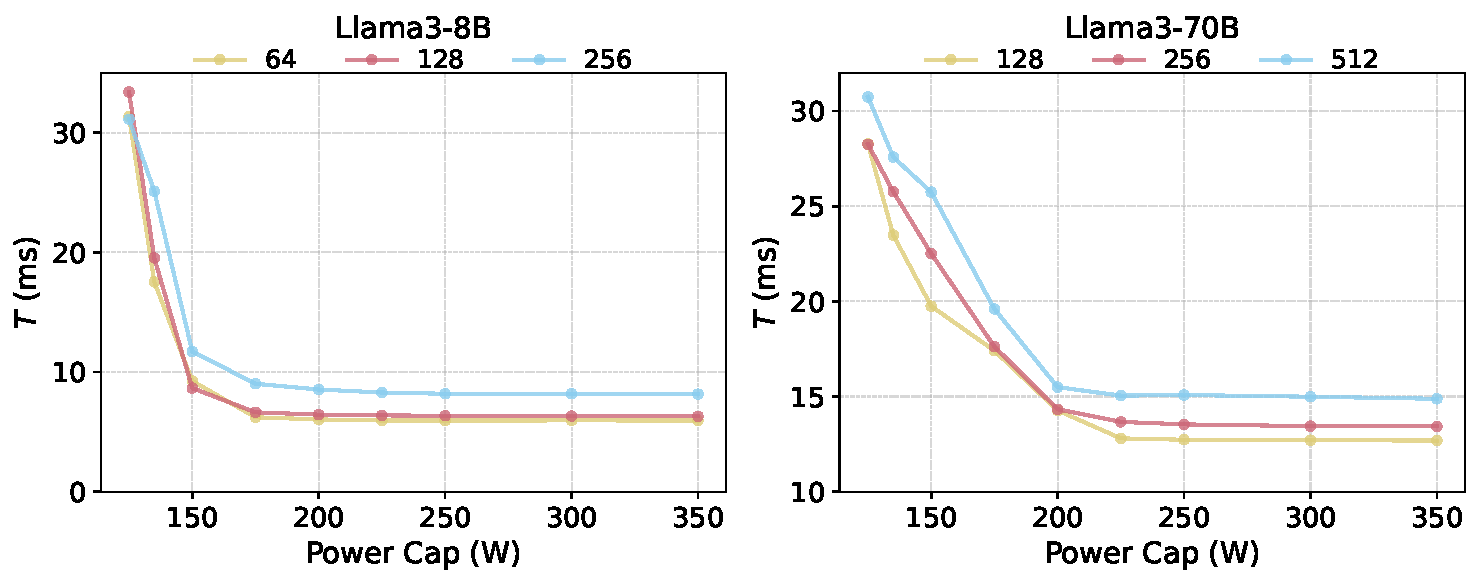
\includegraphics[width=1\linewidth]{figures/execution_time_sampling_new_new.pdf}
%     \caption{Variation of $T$ with different batch size across four Nvidia RTX 3090 GPUs and one NVidia A100 GPU, using Llama3-8B and Llama3-70B on the ShareGPT dataset.}
%     \label{profile_data}
% \end{figure}


We collect data on four NVIDIA RTX 3090 GPUs running Llama3-8B and eight NVIDIA A100 GPUs running Llama3-70B.
The ShareGPT dataset\cite{chiang2023vicuna} was utilized as the primary workload.
During the measurements, we set the frequency for the GPUs in all stages except the last one prior to launching the inference tasks. 
Key timestamps, such as the start and the end for each batch $B_{i,j}^{k}$ across all GPU stages were recorded.

Our analysis focuses specifically on the execution time of every iteration in the first three stages of a batch.
Since the first three stages have the same number of layers and are executed on the same GPU hardware, their execution times are assumed to be the same and stable as discussed in Section~\ref{sec:stableexecutiontime} . 
For simplicity, we denote the execution time of each stage as $T$. 
We subsequently analyzed the relationship between $T$ and $f$ under varying batch sizes.
We conducted multiple experiments with the batch size ranging from \hcwplaceholder{XX} to \hcwplaceholder{XXX}.
For each configuration, the GPU frequency was adjusted from \hcwplaceholder{XXX}Hz to \hcwplaceholder{XXX}Hz.
The detailed results are presented in Figure~\ref{profile_data}.

%实验环境，写好了
% \begin{figure}[t]
%     \centering
%     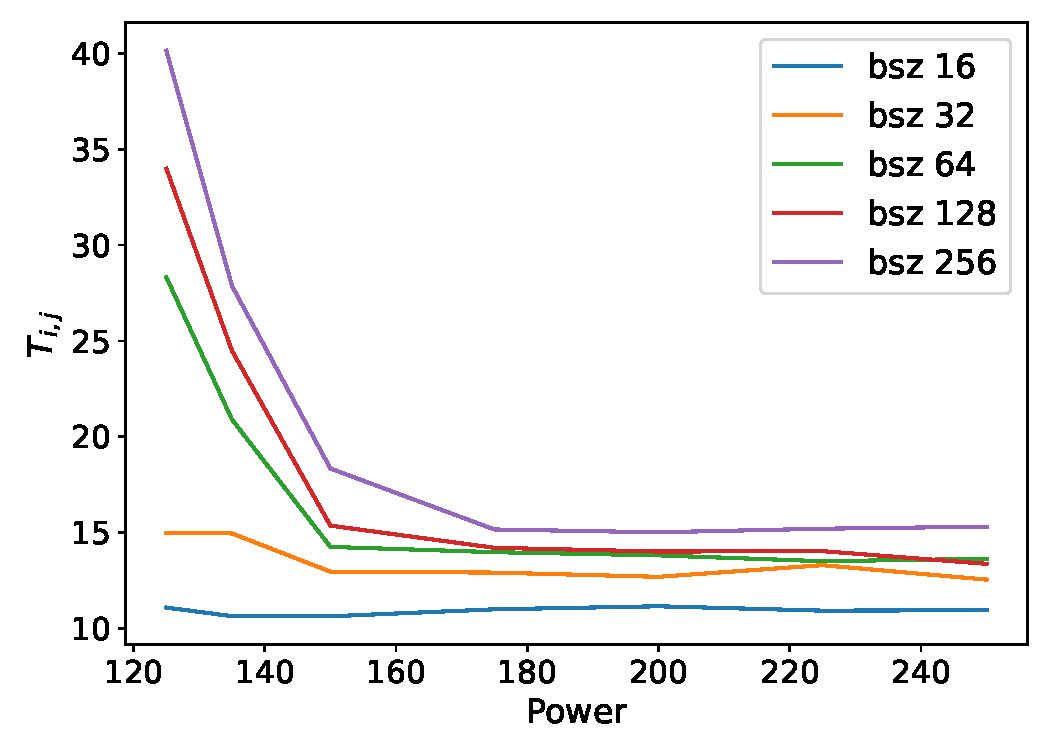
\includegraphics[width=0.8\linewidth]{figures/profile_power.pdf}
%     \caption{The impact of different powers on $T$ at multiple batch sizes}
%     \label{profile_power}
% \end{figure}


Based on the data collected, \thisproj{} was used to build an analytical model for the relationship between $T$ and $f$.
We name it as \textit{TFPrediction Model}.
The model can be formulated as follows: 
\begin{equation}
T=k_1*e^{-k_2f}+k_3
\label{model}
\end{equation} where $k_1$,$k_2$,$k_3$ are coefficients determined by profiling.

% 具体陈述背景ing

We also collect additional data for each batch size to validate the model's effectiveness and to assess its accuracy. By comparing the actual value at each different frequency setting with the value predicted by the \textit{TFPrediction Model}, we found that the \emph{Mean Absolute Percentage
Error (MAPE)} of the predictions is within \hcwplaceholder{XXX}\% on average, which we will further discuss in Section \ref{sec:evaluatecurvefitting}.
It is important to note that, although the batch size can influence the \textit{TFPrediction Model}, its values are discrete rather than continuous making them unsuitable for curve-fitting-based predictions. 
Consequently, the \thisproj{} excludes the batch size as a parameter in the \textit{TFPrediction Model}.



\subsection{Model-Guided Energy Efficiency Optimization}
\label{sec:guide}

Once the analytical model between $T$ and $f$ is established, we can use it to guide the frequency adjustments. 
Based on the analysis in Section~\ref{Principle Model}, the execution time of the last stage $T_{i,N}^{k}$, and the CPU scheduling time $T_S$ are also critical parameters in configuring the frequency.
%The data collected from the profiling and modeling is retained for this purpose. 
Since no frequency adjustment is applied to the GPU that handles the last stage of the inference, its execution time $T_{i,N}^{k}$ remains the same before and after the frequency adjustment.
Similarly, the scheduling time $T_S$, which depends on the time required for each token generation task, is also unaffected. 
This is because the GPU frequency management only slows down each stage to reduce bubbles, but will leave the critical path for the token generation unchanged. 
Thus, $T_S$ is considered constant before and after GPU frequency adjustments.
Based on this observation, all we need is to configure GPU frequency to align $T_{i,1}^{k}$ with $T_{i,N}^{k} - T_S$ and adjust the other stages $T_{i,2}^{k}$ through $T_{i,N-1}^{k}$ to match $T_{i,N}^{k}$.



\subsection{Universality of the Model}
\label{sec:modelportable}


Notably, as the critical parameters of the GPU frequency configuration that include $T$, $T_S$ and the model parameters from the \textit{TFPrediction Model} are collected from profiling, it is important to know how they are affected by the LLM inference execution environment.
It can determine the generalizability of our model, specifically whether it can effectively and efficiently enhance the inference engine with a minimal profiling overhead.

The execution time of an application is generally influenced by its input data and the software and hardware configurations \cite{fu2024serverlessllm,moon2024lpu}. 
For an LLM inference engine, they can be categorized as follows.
\textbf{Input data:} The requests submitted by users, such as the texts of the questions posted, may directly impact the execution time.
\textbf{Software configurations:} Key factors may include the batching strategy, the batch size and the model scale.
% , and other parameters \bygxl{list additional relevant factors here}.
% GPU memory
\textbf{Hardware configurations:} The type and the number of GPUs, which determine the number of pipeline stages, can significantly affect the performance.
Understanding the interplay of these factors is critical in understanding how the key parameters work in \thisproj{}.


Firstly, the input data directly determines the \textit{sequence length} of each request.
As discussed in Section~\ref{sec:stableexecutiontime}, the execution time is generally insensitive to sequence length.
Therefore, we neglect the impact of \textbf{input data} in \thisproj{}.


For the \textbf{Software configuration}, model scale and batch size influence the size of the matrices involved in computation, consequently impacting execution time, as analyzed in Section~\ref{sec:llmandtransformer}.
% Specifically, the model scale dictates the size of the parameter matrix, while the batch size controls the number of rows in the QKV matrix.
\bylyz{Specifically, the model scale determines the size of the parameter matrices, whereas the batch size dictates the size of the input matrices.}
Although these factors have a significant impact on $T$, they are typically determined before the deployment of LLMs and remain fixed throughout the inference process.
Consequently, $T$ requires only an one-time profiling for each combination of the model and the batch size.
In practice, the diversity of LLMs is limited by training cost, and the choice of batch size is constrained by GPU memory, further reducing profiling effort. 



\textbf{Hardware features} also play a critical role in determining the execution time and the energy efficiency of batches. 
% Consequently, re-profiling $T_{i,n}$ becomes necessary when the hardware platform changes.
Consequently, re-profiling $T$ is required when the hardware platform changes.
Similarly, the \textit{TFPrediction Model}, which is vital for predicting batch execution times, is also insensitive to input data. 
% Instead, it is primarily influenced by software configurations such as Model Scale, Batch Size (bsz), and hardware features. 
Instead, it is primarily influenced by software configurations such as model scale, batch size, and hardware features. 
Re-profiling is required whenever these parameters change. 
% However, as the shape of the curve is inherently determined by the characteristics of the GPU, our experiments demonstrated that only six measurements are needed to achieve adequate accuracy for the model.
However, as the shape of the curve is inherently determined by the characteristics of the GPU, our experiments show that only six measurements are needed to achieve adequate accuracy for the model.
% \bygxl{only XXXX measurements are needed to parameterize the model}.

For $T_S$, its execution time is determined by the CPU and the number of requests to be scheduled, which in turn are influenced by both the hardware and the batch size. 
As noted earlier, in an on-going inference, neither the batch size nor the hardware changes. 
Hence, once the operating environment is established, $T_S$ requires only an one-time profiling.


In summary, the batch-level behavior is insensitive to the input data and is primarily influenced by the software configuration and the hardware platform.  
As these parameters remain stable in an ongoing inference environment, a one-time profiling effort is sufficient to ensure the applicability of our model to subsequent inference runs. 




\section{Implementation and Evaluation}
\label{sec:evaluation}

\begin{figure}[t]
    \centering
    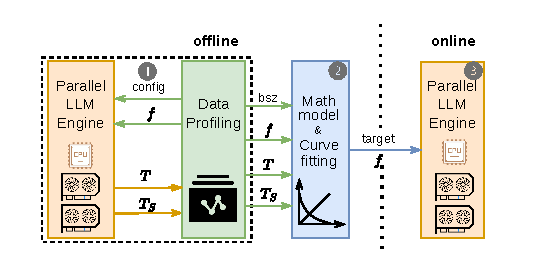
\includegraphics[width=0.8\linewidth]{figures/TACO_Rebuttal/overview_new.pdf}
    \caption{The deployment of \thisproj{}. In the Offline Phase, critical parameters are collected to construct an analytical model. In the Online Phase, the GPU frequency is adjusted based on the model's guidance. }
    \label{overview}
\end{figure}

% We have implemented \thisproj{} on the open-source SARATHI framework \cite{agrawal2024taming} and choose it as baseline.
% SARATHI is built on the widely used LLM inference framework vLLM \cite{kwon2023efficient}, which is the first open-source framework to adopt the continuous batching technique.
% Additionally, SARATHI provides APIs to record the lifecycle of each request in detail, enabling precise data collection and profiling.

\bylyz{
We have implemented \thisproj{} on the open-source SARATHI and SGLang framework.
The former is built on the vLLM and provides AIPs to record the lifecycle of each request in detail for data collectiong and profiling.
The latter is another widely used LLM inference framework, mainly used for XXX.
}

% \begin{figure}[t]
%     \centering
%     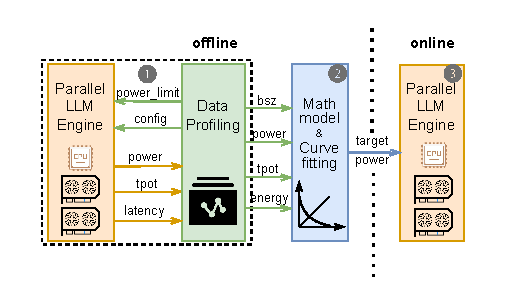
\includegraphics[width=0.7\linewidth]{figures/overview.pdf}
%     \caption{The deployment of \thisproj{}. In the Offline Phase, critical parameters are collected to construct an analytical model. In the Online Phase, the GPU power cap is adjusted based on the model's guidance. }
%     \label{overview}
% \end{figure}

Figure~\ref{overview} shows the implementation and the deployment of the \thisproj{}. 
It consists of two main components: the offline profiling part and the online frequency adjustment part.
During offline profiling part, the deployed LLM engine processes a small number of requests to collect the data for $T_S$ and $T$ under different frequency settings. 
Accordingly, the parameters for the \textit{TFPrediction Model} can also be derived from the collected data. 
Using the method outlined in Section~\ref{sec:guide}, the optimal frequency settings are then determined. 
The model and its setting can be reused for the same model configuration running on the hardware platforms with the same features later.
During online frequency adjustment part, the frequency is configured before the inference process begins, after which the system can operate without further intervention.

% \begin{figure*}[t]
%     \centering
%     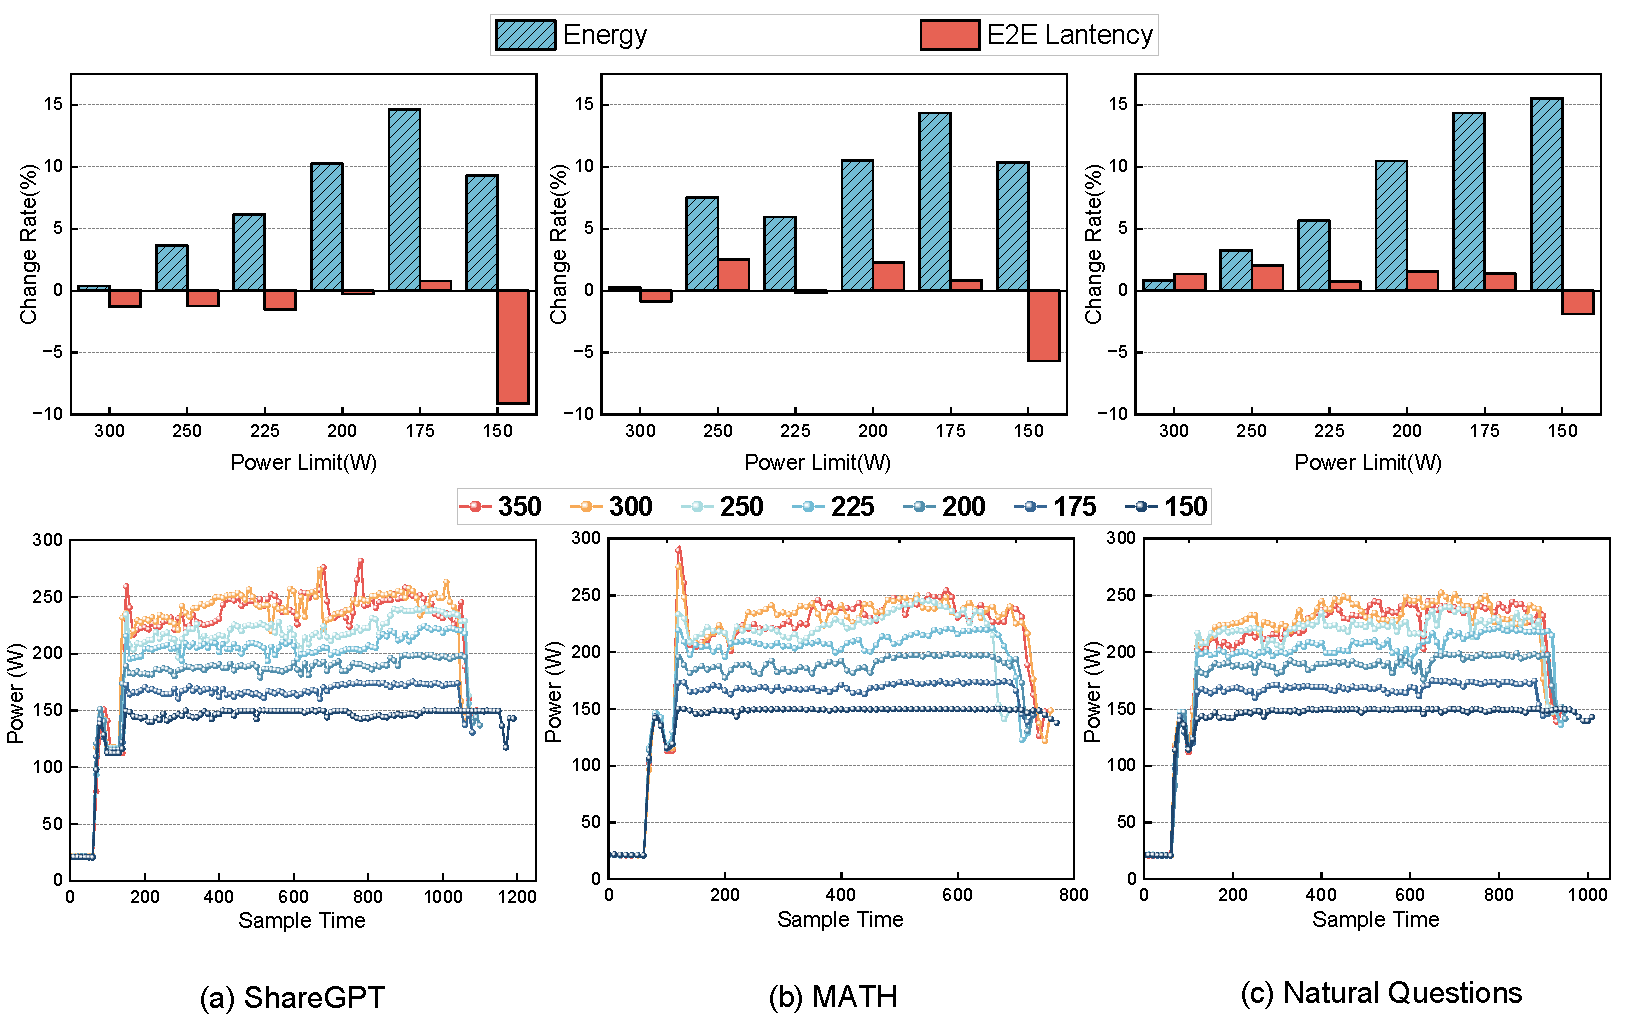
\includegraphics[width=\linewidth]{figures/power_lantency.pdf}
%     \caption{Energy savings and performance variations at different power levels across multiple datasets using the Llama2-7B model. Positive numbers indicate improved performance, while negative numbers indicate decreased performance. Positive numbers indicate energy savings.
%     }
%     \label{latency_energy}
% \end{figure*}

\begin{figure*}[t]
    \centering
    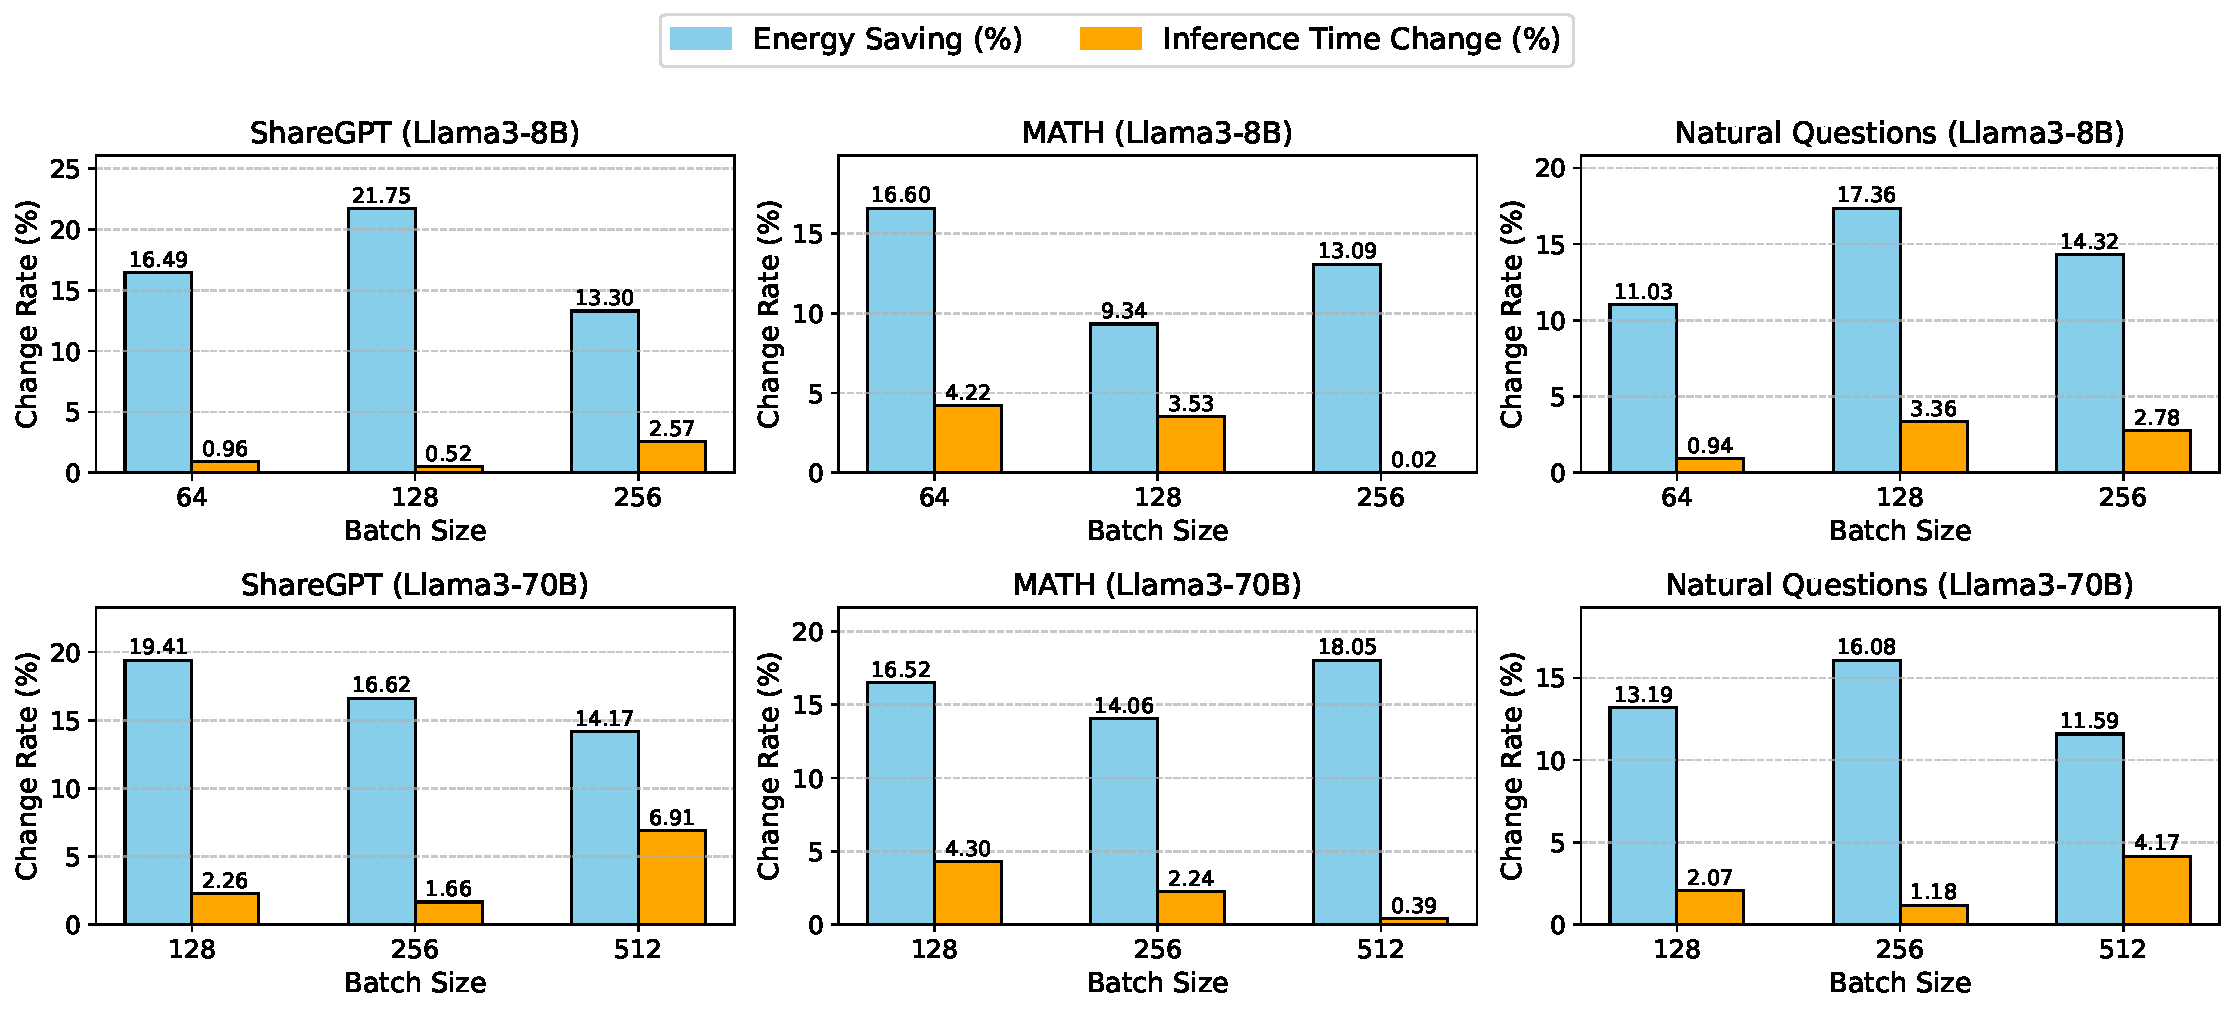
\includegraphics[width=1\linewidth]{figures/Energy_E2E_under_BatchSize_lyz_new_new_new_new_new.pdf}
    \caption{\bylyz{Energy efficiency and performance variations at different power levels across multiple datasets using Llama3-8B model, Llama3-70B and XXX. 
    Positive numbers indicate energy efficiency improvements and performance degradation.
    }\lyzcheck{3*3 Figures similar to this. But add XXX model in the last row. And change the label, with three labels, including energy efficiency, inference time and throughput. The x is Batch Size, and y is Change Ratio. Different row means different model, and different column means different DataSet. }}
    \label{latency_energy}
\end{figure*}



\subsection{Experimental Setup}

\textbf{Hardware.}
The experiments have been conducted on two workstations.
The first is equipped with an Intel Xeon Gold 6326 CPU running at 2.90 GHz and four NVIDIA RTX 3090 GPUs, each with 24 GB of memory.
The second is equipped with Intel Xeon Gold 6348 CPU running at 2.60 GHz and eight A100 GPUs, each with 40 GB of memory.
Both workstations are operating on Ubuntu 22 and have utilized the PyTorch 2.3.0 framework with CUDA 12.4 to leverage GPU acceleration.

% In the experiment, we select two mainstream open-source LLM models for evaluation: Llama3-8B and Llama3-70B.
% % \bylyz{The first two models are executed on the first workstation, while the last is on the second workstation.}
% Llama3-8B is executed on the RTX3090, while Llama3-70B is on A100.
% The workload is derived from three datasets: Natural Questions\cite{kwiatkowski2019natural}, ShareGPT\cite{chiang2023vicuna}, and MATH\cite{hendrycks2021measuring}. 
% The first two datasets are natural language question-answering benchmarks, while MATH focuses on mathematical reasoning. 
% These datasets are widely recognized in the field and are commonly used to evaluate LLM capabilities such as language understanding, reasoning and handling long-context scenarios.
% For every dataset, we randomly select input (i.e., the questions) from the dataset to simulate users' requests.

\bylyz{
\textbf{Model.} In the experiment, we select three mainstream open-source LLM models using BF16 precision for evaluation: Llama3-8B, Llama3-70B, and XX.
Specifically, Llama3-8B is deployed on RTX 3090 GPUs using vLLM, Llama3-70B is deployed on A100 GPUs using SGLang, and XX is deployed on RTX 3090 GPUs using SGLang.
The batch size is set to {64, 128, 256} for Llama3-8B, {128, 256, 512} for Llama3-70B, and {XXX, XXX, XXX} for XX, considering both memory capacity and inference efficiency.
We use CUDA events to record the execution time of each batch, and its average value is utilized as $T$ in the $TFPrediction Model$. 
}

\bylyz{
\textbf{Workload.}
The workload is derived from three datasets: Natural Questions\cite{kwiatkowski2019natural}, ShareGPT\cite{chiang2023vicuna}, and MATH\cite{hendrycks2021measuring}. 
The first two datasets are natural language question-answering benchmarks, while MATH focuses on mathematical reasoning. 
These datasets are widely recognized in the field and are commonly used to evaluate LLM capabilities such as language understanding, reasoning and handling long-context scenarios.
For each dataset, we randomly sample inputs (i.e., user queries) to simulate real-world request patterns.
Specifically, we use XX requests for online evaluation, with a subset of 512 requests randomly selected for offline data profiling.
}

\bylyz{
\textbf{Metrics and Baseline.}
We take the end-to-end inference time and throughput (measured in generated tokens per second, tokens/s) as the key metric to evaluate the performance, while utilizing end-to-end energy consumption to evaluate the energy efficiency. 
For the energy consumption, we sample the real-time power usage of GPUs using the \textit{nvidia-smi} API provided by the NVIDIA GPU Driver at the granularity of 10 ms.
The sampled data is shown as a curve in Figure~\ref{power-runtime}, and the end-to-end energy is computed through the definite integration of the power curve.
To ensure measurement reliability, each experimental configuration is executed XXX times, with the average metrics reported as the final results.
We employ the default automatic DVFS mechanism as our baseline and evaluate our metrics against it.
}

% We use the question-answer pairs from the datasets for online evaluation and randomly select a portion of pairs for offline data profiling.
% In our experiments, the batch size is set to 64/128/256 for Llama3-8B and 128/256/512 for Llama3-70B, considering both memory capacity and efficient inference.
% During the profiling, 512 questions are randomly selected from the dataset as the input to the LLM inference engine.
% The execution time of each batch is recorded, and its average value is used for $T$ in the \emph{TFPrediction Model}. 
% \bylyz{
% We uses the cuda event to record he execution time of each batch, and its average value is used for $T$ in the \emph{TFPrediction Model}. 
% }
% }

% It is worth noting that, due to the CPU–GPU asynchronous execution mechanism in the inference engine, accurately measuring the execution time of individual stages is challenging.
% To address this, we insert explicit synchronization statements (e.g., \texttt{torch.cuda.synchronize}) during offline profiling, which improves the precision of batch execution time measurements.
% For online inference, however, these synchronizations are removed in order to avoid unnecessary stalls and maximize performance.



\subsection{Evaluation}


\begin{figure*}[t]
    \centering
    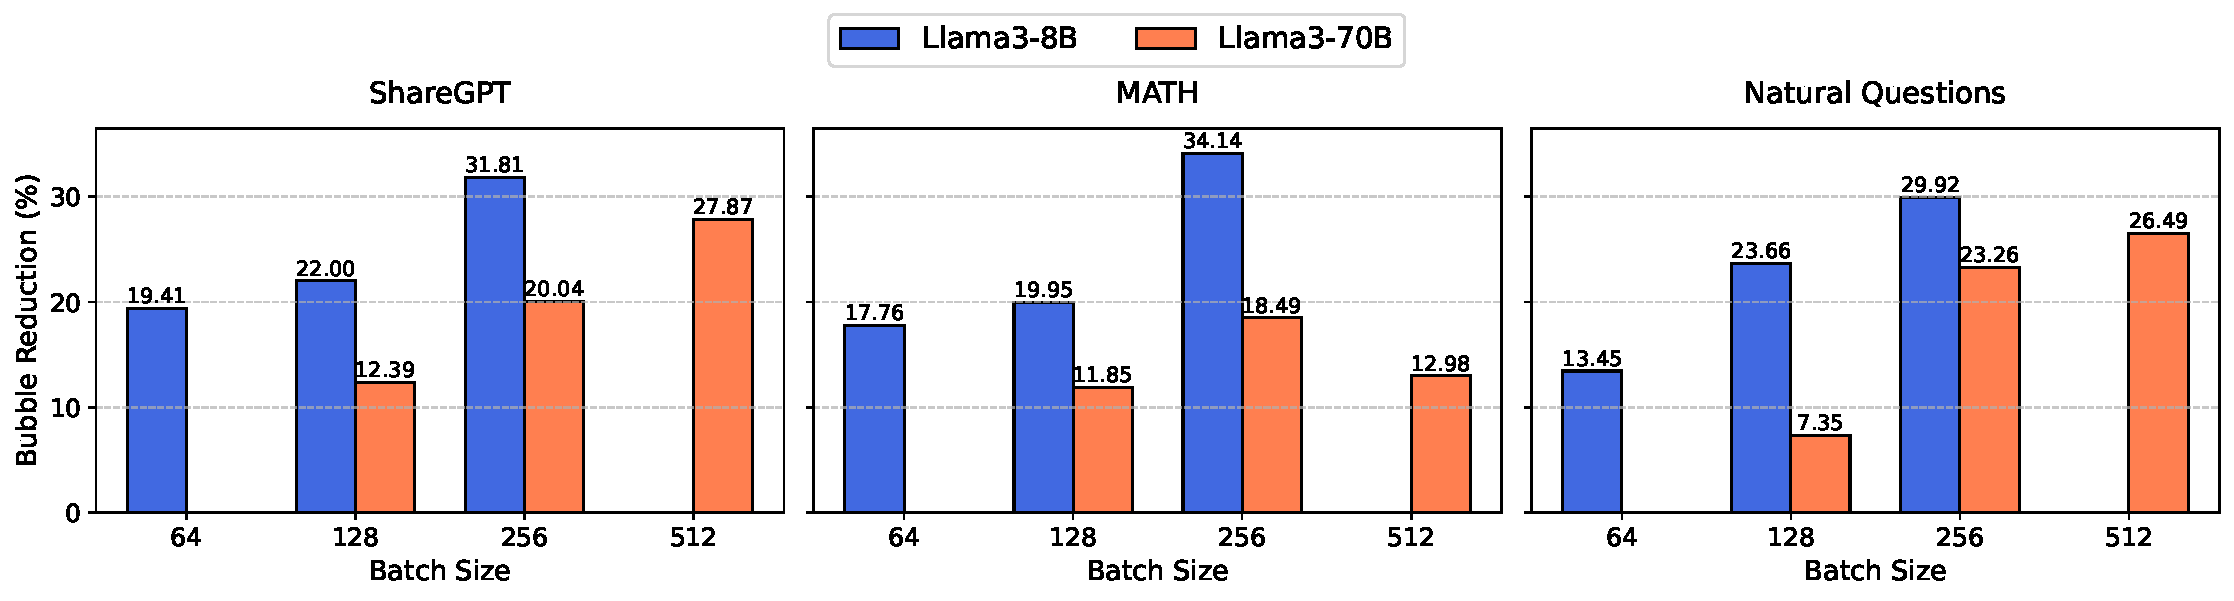
\includegraphics[width=\linewidth]{figures/IDLE_Computing_under_BatchSize_lyz_new_new_new_new.pdf}
    \caption{Percentage of bubble reduction across different batch size and datasets. \lyzcheck{(One figure is a model, x is batchsize, y is bubble reduction, different color means different dataset.)}}
    \label{IDLE_Computing}
\end{figure*}



% We take the end-to-end inference time and the energy consumption as the key metrics to evaluate the performance and the energy efficiency of the LLM inference system. 
% Specifically, the end-to-end inference time measures the time from the start of the first batch to the completion of all batches. 
% This also corresponds to the total execution time of the GPU that processes the last stage of the pipeline, i.e., GPU$_4$ as shown in Figure~\ref{timeline}.
% For the energy consumption, we sample the real-time power usage of GPUs using the \textit{nvidia-smi} API provided by the NVIDIA GPU Driver.
% The sampled data is shown as a curve in Figure~\ref{power-runtime}, and the total energy is computed through the definite integration of the power curve.
% \bylyz{
% We adopt the automatic DVFS mechanism as our baseline and compare these metrics against it.
% }



\subsubsection{Performance and Energy Efficiency}

\begin{table}
  \caption{\lyzcheck{The optimal frequency settings and \textit{TFPrediction Model} coefficient solved by \thisproj{}.}}
  \label{tab:fsettings}
  \begin{tabular}{ccccc}
    \toprule
    Model & 512 & 256 & 128 & 64 \\
    \midrule
    Llama3-8B & -- & 5.39\%  & 4.40\%  & 1.71\%  \\
    Llama3-70B & 6.75\% & 3.12\% & 1.75\% & --  \\
    \bottomrule
  \end{tabular}
\end{table}

In Figure~\ref{latency_energy}, it shows the impact of \thisproj{} on the performance and energy efficiency for Llama3-8B, Llama3-70B and XXX across different datasets compared with DVFS. 
For simplicity of comparison, we normalized the data against the baseline.
The above bars in the figure represent the energy efficiency improvement and performance degradation.
\lyzcheck{Table\ref{tab:fsettings} shows the corresponding optimal frequency solved by \thisproj{}}
The results demonstrate that \thisproj{} consistently achieves significant energy efficiency improvements across all three datasets, regardless of the batch size and the LLM model.

Notably, the energy efficiency improvements reach their highest at XXX\% with the batch size of XXX on the XXX dataset using the XXX model.
Across all three datasets and on average, XXX\% improvements can be achieved for the Llama3-8B, XXX\% for the Llama3-70B and XXX\% for the XXX.
This is also reflected by the minimal performance variation observed across different batch sizes.
Given that batch size is typically constrained by the GPU memory capacity in real-world scenarios, these results show that \thisproj{} can function well under varying memory limitations.

The XXX bars and XXX bars in the figure show the inference time and throughput variations respectively. 
Positive values indicate an decrease in the performance, whereas shorter bars signify better.
%These variations may result from model deviations, 
These variations may be caused by the imprecision of the analytical model, which can lead to an overestimation of pipeline bubbles and subsequent over-adjustment of the frequency.
%which can introduce performance overhead.
Nevertheless, the results show that the introduced fluctuation in the performance is quite minimal—approximately XX\% and XX\% on inference time and throughput on average—indicating that the analytical model is quite accurate and the impact of the energy efficiency improvement on the inference time is rather small.
% For those bars below zero, they are mostly caused by the performance variation and the measurement noises during the LLM inference.
Besides, inherent performance variations and the measurement noises can also cause the system’s performance to fluctuate to some extent.
% For those bars exhibiting slightly larger variations, they may also be caused by the performance variation and the measurement noises during the LLM inference.


% To further investigate the impact of power cap on the system, we select a specific inference engine configuration and enumerate different power cap.
To further investigate the impact of frequency adjustment on the system, we select a specific inference engine configuration and evaluate it under different frequency settings.
We vary the frequency from XXX to XXX in an increment of XXX for the Llama3-70B and XXX, using XXX dataset.
In each setting, inference time and energy consumption are measured.
The results are shown in Figure~\ref{power_lantency_math}.
As the frequency decreases (from XXX to XXX), a larger proportion of pipeline bubbles is mitigated, resulting in sustained energy efficiency improvement, while the overall system performance remains largely unaffected.
However, when the frequency falls below a critical threshold (from XXX to XXX), the execution time of the preceding stages surpasses that of the last stage, thereby becoming the system's bottleneck.
Consequently, system performance drops sharply, and the associated energy efficiency improvement diminish, potentially resulting in negative gains.

\bylyz{
Table shows our solved frequency settings using \thisproj{}.
It shows that ...(some analysis).
% It also shows that the optimal frequency setting lies between XXX and XXX, with the optimal value close to XXX.
% We use \thisproj{} to calculate the frequency that exactly matches the execution time of the preceding stage to the last stage.
% The predicted frequency is XXX, which closely aligns with the experimental results.
}

\subsubsection{Reduction of Bubbles}
\label{sec:evaluatebubble}

% \begin{figure*}[t]
%     \centering
%     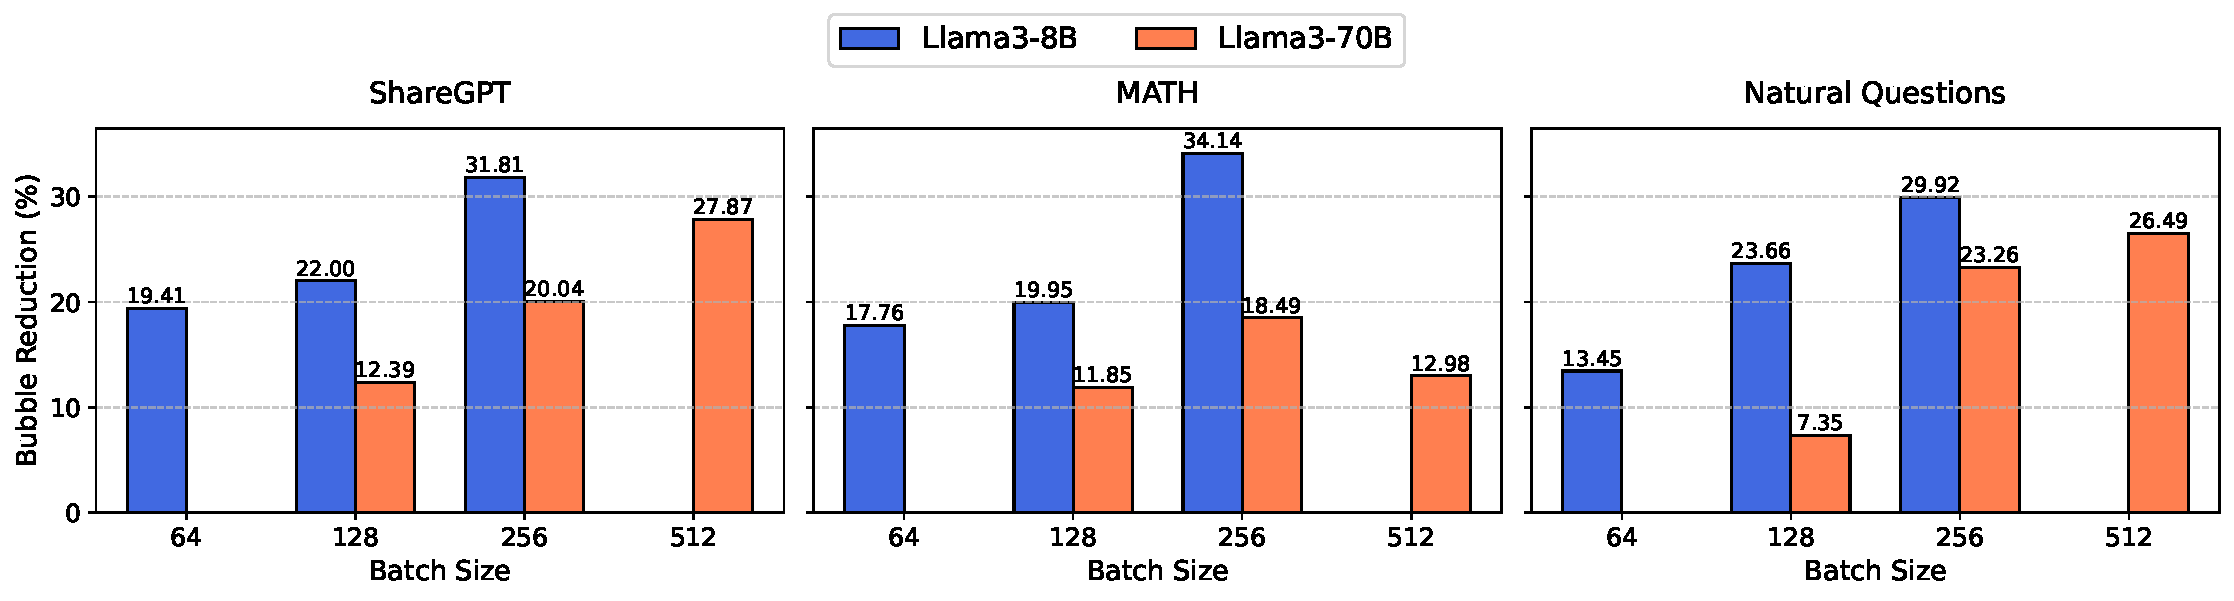
\includegraphics[width=\linewidth]{figures/IDLE_Computing_under_BatchSize_lyz_new_new_new_new.pdf}
%     \caption{Percentage of bubble reduction across different batch size and datasets.}
%     \label{IDLE_Computing}
% \end{figure*}

% Figure 13
% \begin{figure}[t]
%     \centering
%     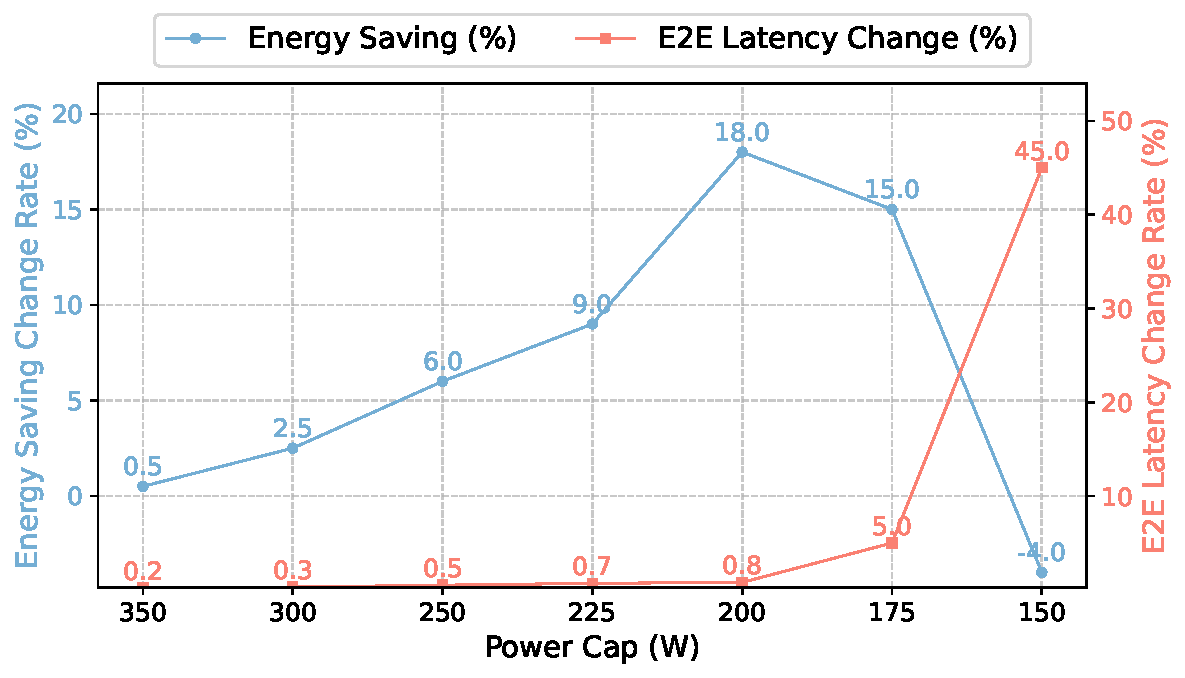
\includegraphics[width=0.9\linewidth]{figures/power_lantency_math_lyz_new_new_new.pdf}
%     \caption{Latency and energy reduction on the MATH dataset using Llama3-70B and a batch size of 512 with different power cap settings.}
%     \label{power_lantency_math}
% \end{figure}

% Figure 14
% \begin{figure}[t]
%     \centering
%     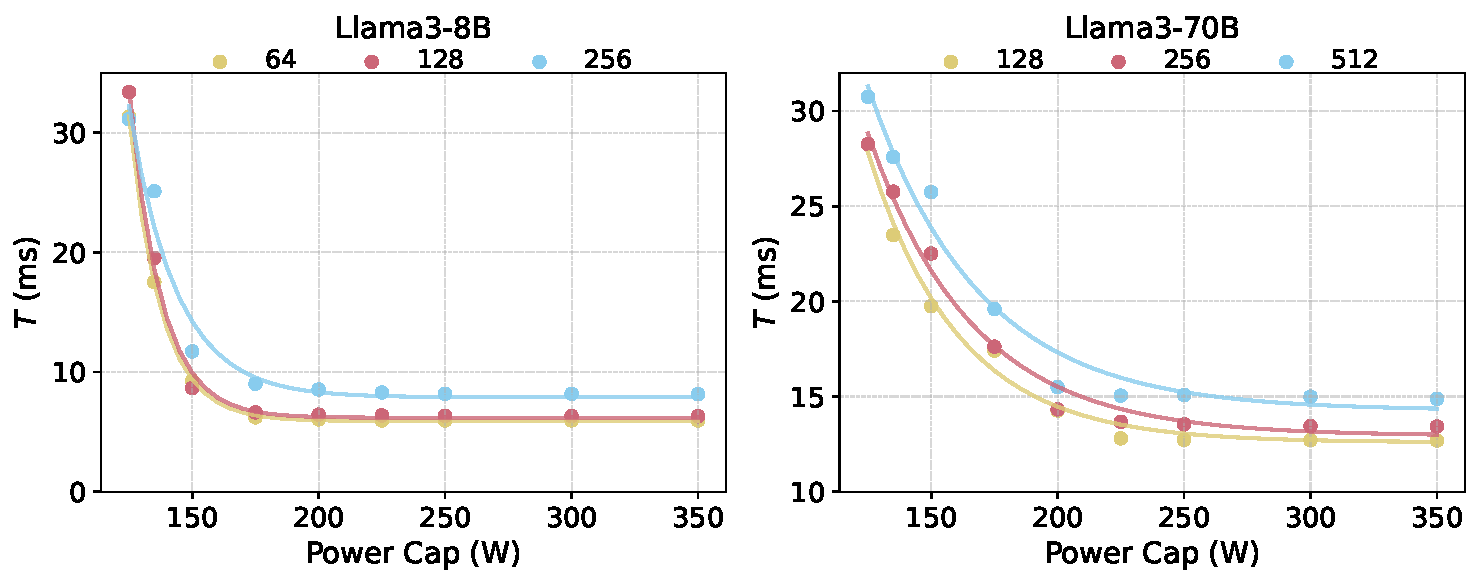
\includegraphics[width=\linewidth]{figures/execution_time_prediction_new_new.pdf}
%     \caption{Curve fitting for the relationship between power cap $P$ and batch stage execution time $T$ across different batch size, models, and platforms. The scatter points represent actual measured values, while the curves are derived from the fitted model.}
%     \label{fig:curvefit}
% \end{figure}


% Figure 13 and 14
\begin{figure}[t]
    \centering
    \begin{minipage}[t]{0.48\textwidth}
        \centering
        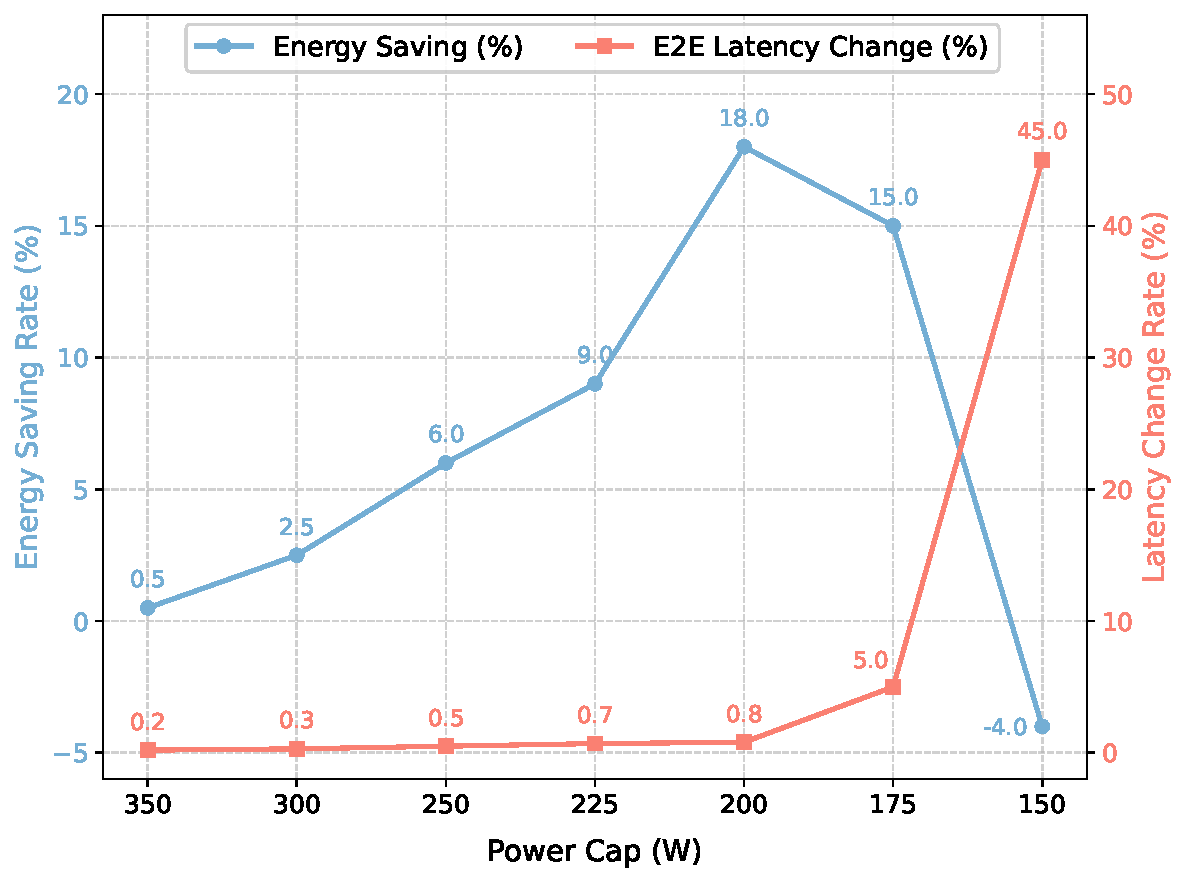
\includegraphics[width=\textwidth]{figures/power_lantency_math_lyz_new_new_new_new_new_new.pdf}
        \caption{\bylyz{Enegry efficiency and performance variations on the XXX dataset using Llama3-70B (batchsize: XX) and XXX (batchsize: XX) with different frequency settings.
        \lyzcheck{(Two figures. The top is about Llama3-70B, while the bottom is about XXX. The X is Frequency Settings and left y is Energy Efficiency and right y is Inference Time.(There use the actual value not percentage.))}}}
        \label{power_lantency_math}
    \end{minipage}
    \hspace{0.02\textwidth}
    \begin{minipage}[t]{0.48\textwidth}
        \centering
        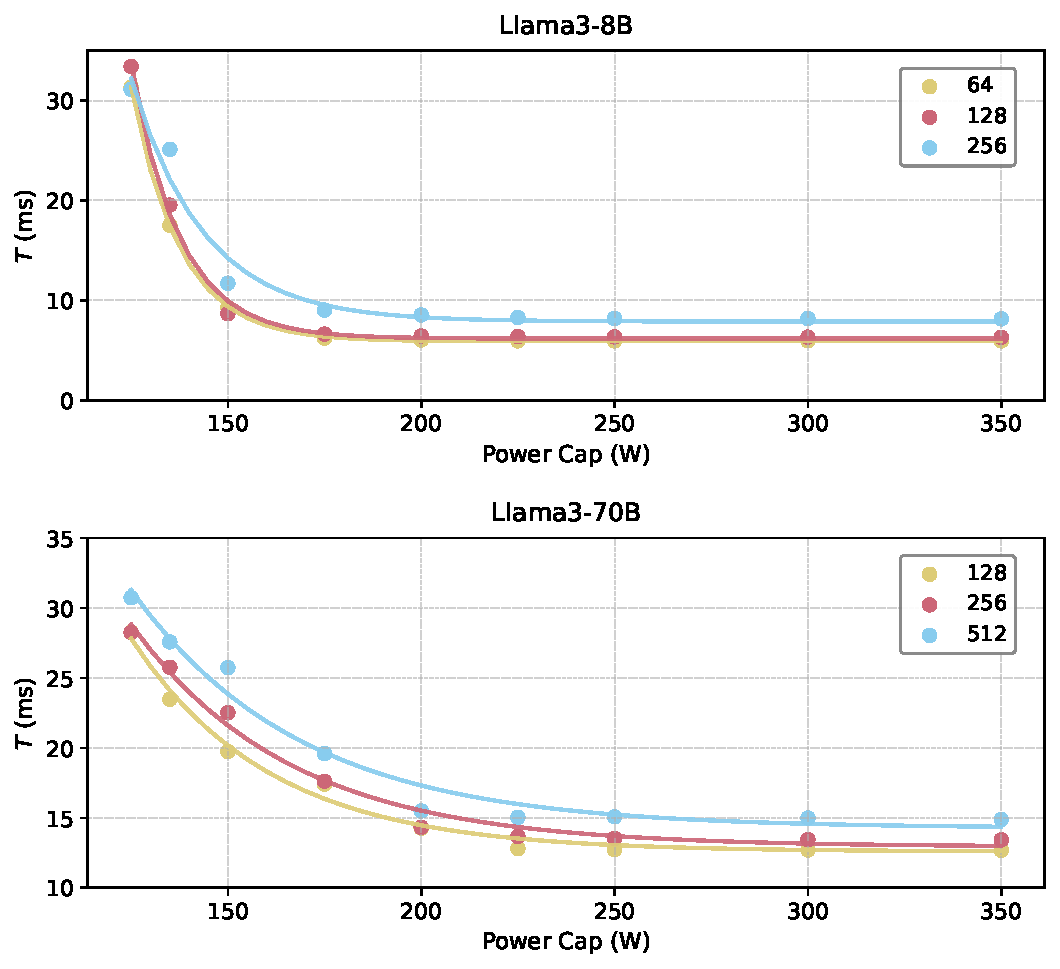
\includegraphics[width=0.87\textwidth]{figures/execution_time_prediction_new_new_new.pdf}
        \caption{Curve fitting for the relationship between frequency $f$ and stage execution time $T$ across different batch size, models, and platforms. The scatter points represent actual measured values, while the curves are derived from the fitted model.
        \lyzcheck{Three figures, left Llama3-8B, middle Llama3-80B, right XXX. The x is $f$, the y is $T$. Different Color Means different Batch Size.}
        }
        \label{fig:curvefit}
    \end{minipage}
\end{figure}

% Figure 13 and 14
% \begin{figure}[t]
%     \centering
%     % 使用 [b] 确保两个 Caption 的顶端是对齐的，视觉上更整齐
%     \begin{minipage}[b]{0.48\linewidth}
%         \centering
%         % 统一限制高度（如 3.8cm），keepaspectratio 防止变形
%         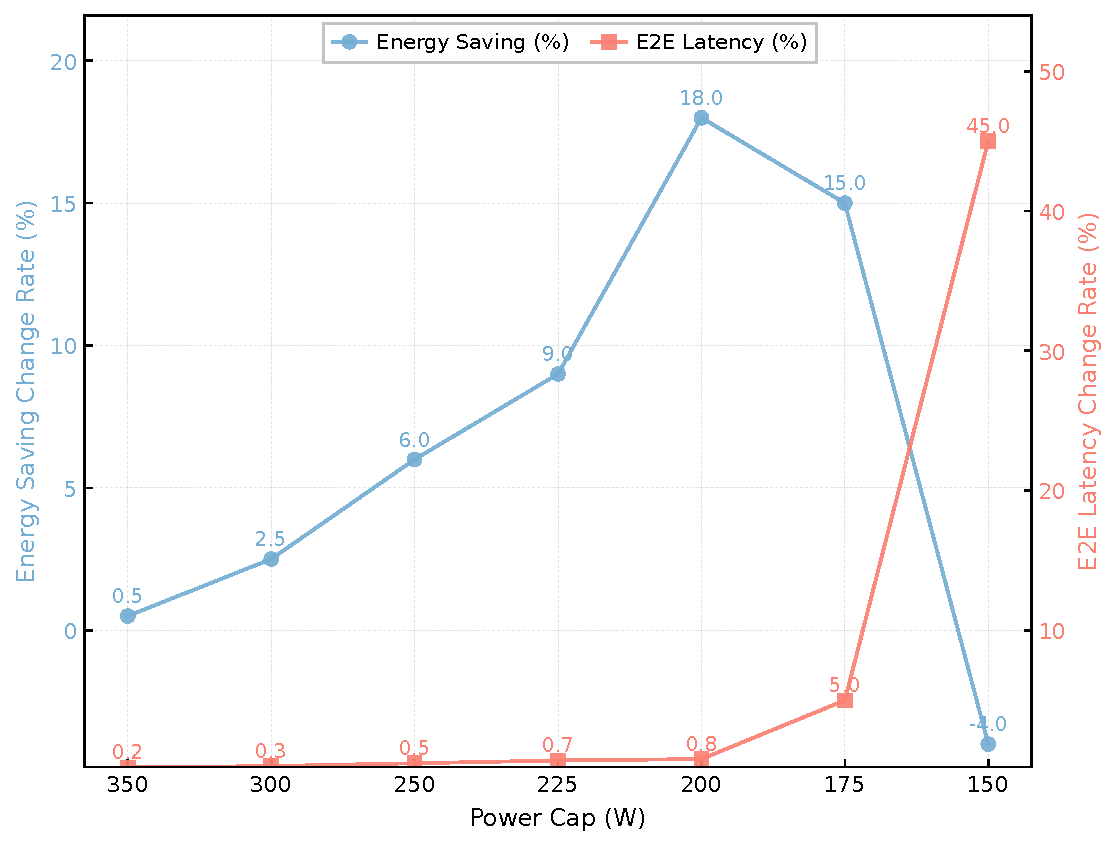
\includegraphics[width=\linewidth, height=3.8cm, keepaspectratio]{figures/power_lantency_math_lyz_new_new_new_new.pdf}
%         \vspace{-6pt} % 缩小图片与标题之间的空隙
%         \caption{\small Latency and energy reduction on the MATH dataset.} % 建议精简标题，详细描述放正文
%         \label{power_lantency_math}
%     \end{minipage}
%     \hfill % 自动撑开左右间距
%     \begin{minipage}[b]{0.48\linewidth}
%         \centering
%         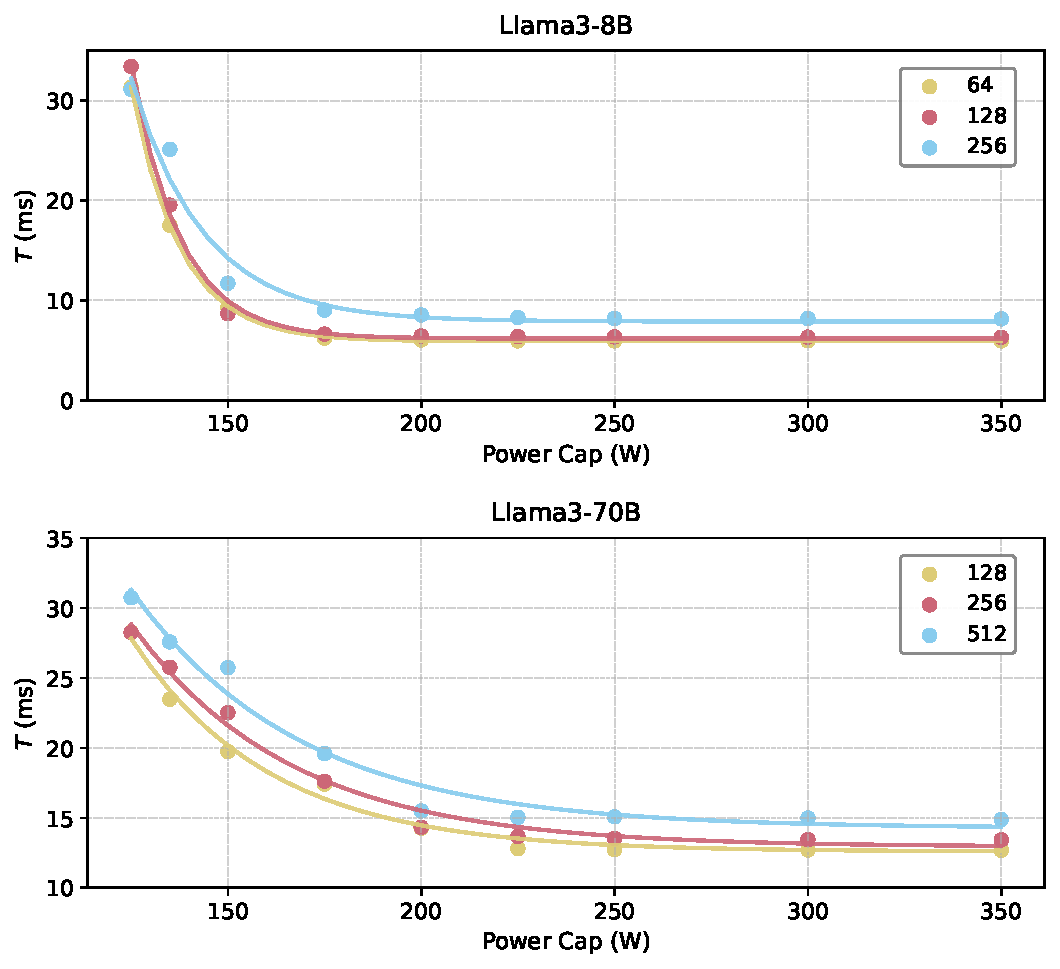
\includegraphics[width=\linewidth, height=3.8cm, keepaspectratio]{figures/execution_time_prediction_new_new_new.pdf}
%         \vspace{-6pt}
%         \caption{\small Curve fitting for power cap $P$ and stage time $T$.}
%         \label{fig:curvefit}
%     \end{minipage}
% \end{figure}

To further understand the energy efficiency improvement, we evaluate the proportion of pipeline bubbles before and after the adjustment of the frequency settings using \thisproj{} to verify its impact on the pipeline performance. 
Figure~\ref{IDLE_Computing} shows the percentage of reduction across multiple datasets and batch size.
In the experiment, we record the start and the end time of every batch in each stage. 
In each stage, the duration between the end time of a batch and the start time of the following batch is identified as a pipeline bubble.
While the duration between the start time of the first batch in the first stage and the end time of the last batch in the final stage is recorded as the total execution time for the inference.
Finally, the percentage of the time consumed by pipeline bubbles is calculated.
The figure illustrates the reduction in the pipeline bubbles under various conditions. 

The most significant reduction occurs with a batch size of XXX and XXX dataset on XXX that reaches XXX\%. 
On average, a XXX\% reduction in bubbles can be achieved across three datasets and various batch sizes using the Llama3-8B model, XXX\% on Llama3-70B and XXX\% on XXX.
This demonstrates that lowering frequency can effectively extend the computation time to squeeze out bubbles and reduce their proportion in the pipeline without affecting the total inference time.

It is important to note that GPU idle time is not solely caused by pipeline bubbles. 
Factors such as communication delays, abnormal requests with extremely long contexts, and the asynchronous execution mechanism also contribute to GPU idling. 
Consequently, it is not possible to completely eliminate GPU idle time using \thisproj{}.


\subsubsection{Model Accuracy and Universality}
\label{sec:evaluatecurvefitting}


We also evaluate the accuracy of the \textit{TFPrediction Model} to validate its ability to correlate the performance and its energy efficiency across various configurations including different batch size. 
%The evaluation involves comparing the model's prediction with the actual data to ensure that it accurately represents the system's behavior under different conditions.
%
Note that, as discussed in Section 3.2, we purposely exclude the batch size as a parameter used in the \emph{TFPrediction Model} because of its discrete nature.

The results are illustrated in Figure~\ref{fig:curvefit}. 
In the figure, each point of different colors represents the average execution time, denoted as $T$ in the \emph{TFPrediction Model}, for a specific batch size and frequency setting.
The curve of the same color represents the values predicted using the \textit{TFPrediction Model}.
%results generated through the curve-fitting process.
%The figure demonstrates 
It shows a high degree of agreement between the predicted value and the measure data point, validating the effectiveness of the curve-fitting method used in \thisproj{}.

To further validate the accuracy and the universality of \thisproj{}, a dataset is constructed for each batch size on an LLM by combining the measured results from all three datasets.
In each measurement, the frequency $f$ and the average batch execution time $T$ are recorded.
For each batch size and model, we make 11 measurements and collect 11 pairs of $f$ and $T$ for each dataset.
In a dataset, 60\% of the data is randomly selected for the curve fitting, while the remaining data is used to evaluate the resulted curve. 
We then calculate their \emph{Mean Absolute Percentage Error (MAPE)}.

\begin{table}
  \caption{Mean absolute percentage errors (MAPEs) of different batch size and LLM models using the ShareGPT dataset (lower is better).}
  \label{tab:mape}
  \begin{tabular}{ccccc}
    \toprule
    Model & 512 & 256 & 128 & 64 \\
    \midrule
    Llama3-8B & -- & 5.39\%  & 4.40\%  & 1.71\%  \\
    Llama3-70B & 6.75\% & 3.12\% & 1.75\% & --  \\
    \bottomrule
  \end{tabular}
\end{table}


% \bygxl{
The results are shown in Table~\ref{tab:mape}. 
% For the evaluated models of Llama3-8B and Llama3-70B, it achieves an MAPE as small as 6.75\% across all batch sizes. 
For the evaluated models, including Llama3-8B, Llama3-70B and XXX, it achieves an MAPE as small as 3.85\% on average. 
This demonstrates the stability of the correlation between $f$ and $T$, indicating that only 6 samples are sufficient to construct the model. 
Such lightweight profiling simplifies the deployment of the \thisproj{} framework.
Together with the high accuracy in predicting and setting the power caps, they make the \thisproj{} framework very practical and effective for pipelined-based LLM models running on most existing system configurations to achieve a good balance between the high performance and energy efficiency.


\section{Related Works}
\label{sec:relatedworks}

%\bygxl{Follow the list below}
%1. scheduling, batch scheduling, continuous batching
%2. power management of GPU, Power management of LLM

\textbf{Pipeline Scheduling in LLMs.} 
Pipeline parallelism is widely adopted in frameworks such as FedPipe~\cite{fang2024automated}, PipeLLM~\cite{ma2023poster}, and CEBench~\cite{sun2024cebench} to address GPU memory limits that prevent single-device model hosting.
To maximize resources, systems like DeepSpeed~\cite{aminabadi2022deepspeed}, vLLM~\cite{kwon2023efficient}, and PyTorch~\cite{paszke2019pytorch} use batch scheduling.
Eliminating pipeline bubbles is key to performance optimization.
Prior works~\cite{arfeen2024pipefill, zheng2024response, lin2024syncintellects} focus on batch alignment, while micro-batching~\cite{athlur2022varuna, narayanan2019pipedream} enables smaller, parallelized batches.
Continuous batching, from Orca~\cite{yu2022orca}, schedules at token-level granularity to minimize misalignment bubbles and is adopted in vLLM~\cite{kwon2023efficient} and Sarathi~\cite{agrawal2024taming}.
However, we show that inherent bubbles from compute-memory mismatches cause significant energy waste.
We address this by controlling the frequency to extend computation time and reduce bubbles.

\noindent
\textbf{GPU Energy Effiency.}
Dynamic Voltage and Frequency Scaling (DVFS) dynamically adjusts CPU voltage and frequency to optimize energy efficiency, and has been extended to GPUs~\cite{mei2013measurement, tang2019impact, kakolyris2024slo, jia2024pccl}.
Research, such as~\cite{guerreiro2019dvfs}, shows DVFS achieves 16\% average energy improvements at the workload level.
% Power-capping techniques~\cite{zhao2023sustainable, patel2024characterizing, stojkovic2024towards} significantly reduce LLM inference energy, while TAPAS~\cite{stojkovic2025tapas} demonstrates power-capping prevents overheating and power failures.
% Recent work~\cite{kakolyris2025throttll} optimizes GPU energy in LLMs by dynamically adjusting frequency based on batch size and KV cache usage.
% In contrast, \thisproj{} targets energy waste from millisecond-scale pipeline bubbles, using static power-capping to extend batch execution time and eliminate bubbles.
% Its model-guided approach ensures energy efficiency without compromising throughput, orthogonal to~\cite{kakolyris2025throttll}.
% Recent work~\cite{kakolyris2025throttll} optimizes GPU energy in LLMs by dynamically adjusting frequency based on batch size and KV cache usage.
% Similarly, Perseus~\cite{chung2024reducing} dynamically scales frequencies for computations on non-critical paths during training to achieve energy savings.
% However, we observe that during inference, the duration of pipeline bubbles aligns with the overhead of dynamic GPU frequency adjustments, making it challenging to eliminate these bubbles.
% In contrast, \thisproj{} targets energy waste from these millisecond-scale bubbles through static power capping, which extends batch execution times to eliminate bubbles while preserving GPU smart power management via DVFS.
Recent work throttLL’eM~\cite{kakolyris2025throttll} examines the impact of GPU frequency and environmental factors on performance and energy consumption, employing dynamic frequency scaling to enhance energy efficiency.
In contrast, \thisproj{} addresses pipeline bubbles arising from workload imbalances in pipeline parallelism.
Perseus~\cite{chung2024reducing} dynamically scales frequencies for non-critical-path computations during training and models the energy-time relationship for each computation to inform scaling decisions.
However, we observe that pipeline bubbles during inference are considerably shorter, typically lasting several to tens of milliseconds, which aligns with the overhead of frequency adjustments.
Consequently, \thisproj{} adopts static frequency setting to avoid constant frequency adjustment and reduce energy consumption.
Furthermore, we model the relationship between iteration time and frequency during inference to guide frequency settings; unlike Perseus, our approach incorporates the effects of batch size and sequence length, yielding a more granular and precise model.








\section{Discussion}
\label{sec:discussion}

\bylyz{
Practical LLM deployments can combine pipeline parallelism (PP) with tensor parallelism (TP) or expert parallelism (EP). 
In such configurations, GPUs can be organized into groups, with PP across groups and TP or EP within each group. 
Additional postprocessing in the last group can still create load imbalance across groups. 
\thisproj{} could be extended to these configurations by profiling group execution times and selecting appropriate frequencies for GPUs in non-critical groups. 
Keeping the last group's frequency settings unchanged and slowing other groups within their available slack could also optimize energy effiency without sacrificing performance.
}

% \bygpt{
% Practical LLM deployments can combine pipeline parallelism (PP) with tensor parallelism (TP) or expert parallelism (EP). In such configurations, GPUs can be organized into groups, with PP across groups and TP or EP within each group. Additional postprocessing in the last group can still create load imbalance across groups. \thisproj{} could be extended to these configurations by profiling group execution times, including communication within each group, and selecting appropriate frequencies for GPUs in non-critical groups. Keeping the last group's frequency settings unchanged and slowing other groups only within their available slack could reduce energy consumption without creating new bottlenecks.
% }

% \bygemini{
% Real-world scenarios typically involve a combination of parallel strategies, including Pipeline Parallelism, Tensor Parallelism, Expert Parallelism, and others. \thisproj{} is equally applicable to these hybrid parallel configurations. Such parallel combinations generally partition GPUs into multiple groups, where inter-group communication employs Pipeline Parallelism, while intra-group communication utilizes Tensor or Expert Parallelism. However, workload imbalances persist across these groups because the last group computes additional postprocessing tasks. Consequently, we can profile and set appropriate frequencies for all groups except the last one to achieve energy savings.
% }

\bylyz{
\thisproj{} specifically targets the workload imbalance resulting from the postprocessing phase. The severity of this workload imbalance dictates the potential effectiveness of our optimization. In most scenarios, the cost of postprocessing is substantial due to the large vocabulary size required for next-token generation. Consequently, this pronounced imbalance serves to provide ample headroom and opportunity for our optimization.
}

% \bygpt{
% \thisproj{} targets load imbalance caused by postprocessing in the final pipeline stage. Its potential benefit therefore depends on the amount of available slack in non-critical stages. For models with large vocabularies, output projection can impose substantial computational overhead on the final stage. When this additional work leaves earlier stages waiting, \thisproj{} can exploit the resulting slack by lowering their frequencies to save energy.
% }

% \bygemini{
% \thisproj{} specifically targets the workload imbalance resulting from the postprocessing phase. The severity of this workload imbalance dictates the potential effectiveness of our optimization. In most scenarios, the cost of postprocessing is substantial due to the large vocabulary size required for next-token generation. Consequently, this pronounced imbalance serves to provide ample headroom and opportunity for our optimization.
% }

\section{Conclusion}
\label{sec:conclusion}

This paper tackles energy inefficiencies in LLM inference due to pipeline bubbles caused by GPU compute-memory mismatches.
We propose \thisproj{}, a framework that uses GPU frequency scaling to align stage execution times, effectively reducing bubbles.
Through a data-driven model of frequency and stage execution time, \thisproj{} applies static frequency adjustments, achieving up to \hcwplaceholder{XXX}\% energy efficiency improvements (average \hcwplaceholder{XXX}\% for Llama3-8B, \hcwplaceholder{XXX}\% for Llama3-70B) with minimal performance impact in pipeline-parallel systems.




%%
%% The acknowledgments section is defined using the "acks" environment
%% (and NOT an unnumbered section). This ensures the proper
%% identification of the section in the article metadata, and the
%% consistent spelling of the heading.
\begin{acks}
This work was supported in part by Natural Science Foundation of China~(62372254),  Innovative Development Joint Fund Key Projects of Shandong NSF (ZR2023LZH003), Beijing-Tianjin-Hebei Basic Research Cooperation Project of Hebei Natural Science Foundation under Grant F2024203115(24JCZXJC00160 in Tianjin). 
\end{acks}

%%
%% The next two lines define the bibliography style to be used, and
%% the bibliography file.
\bibliographystyle{ACM-Reference-Format}
\bibliography{sample-base}

\end{document}
\endinput
%%
%% End of file `sample-manuscript.tex'.
